\documentclass[a4paper,12pt,openany,hyperfootnotes,hidelinks]{scrbook}
\usepackage[utf8]{inputenc}
\usepackage[titletoc,title]{appendix}
\usepackage[linedheaders,parts,pdfspacing,manychapters]{classicthesis}
\usepackage[]{fullpage}
% \usepackage[standardsections]{scrhack} % https://tex.stackexchange.com/questions/511049/conflict-between-titlesec-package-and-scrbook-class-after-most-recent-update-of
\usepackage[section=chapter,numberedsection,acronym,toc, nonumberlist,index]{glossaries}
\usepackage[stylemods=bookindex,abbreviations]{glossaries-extra} % index style
%
\usepackage{amsmath}
\usepackage{amsthm}
\usepackage{amssymb}
\usepackage{style/rest-api}
\usepackage{style/lst}
\usepackage{verbatim}
\usepackage{enumitem}
\setlist{noitemsep}
% \setlist[1]{labelindent=\parindent} % < Usually a good idea
\setlist[itemize]{label={---}}
\usepackage{multirow}
\usepackage{epigraph} % quotations (at start of chapter)
\usepackage{csquotes}
\usepackage{tikz}
\usetikzlibrary{arrows.meta,fit,positioning,shapes}
% \usetikzlibrary{matrix,arrows.meta,fit,positioning,shapes,automata}
% \usepackage{forest}
%
% \usepackage{breakcites} % splits long citations to several lines
% \newcolumntype{L}{>{\raggedright\arraybackslash}X}
%
\setcounter{tocdepth}{2}
%
\let\headheight=\baselineskip
\setlength{\parindent}{0pt}
\setlength{\parskip}{\baselineskip}
\interfootnotelinepenalty=10000 %% Completely prevent breaking of footnotes
%
% %%%%%%%%%%%%%%%%%%%%%%%%%%%%%%%%%%%%%%%%%%%%%
% centered verbatim command
\usepackage{varwidth}
\newenvironment{centerverbatim}{%
  \par
  \centering
  \varwidth{\linewidth}%
  \verbatim
}{%
  \endverbatim
  \endvarwidth
  \par
}
%%%%%%%%%%%%%%%%%%%%%%%%%%%%%%%%%%%%%%%%%%%%%
% make first use \emph
% see: https://tex.stackexchange.com/questions/449104/how-to-style-first-acronym-and-first-glossary-appearance
\newcommand{\firstuseformat}[1]{\emph{#1}}
%
\renewcommand{\glslinkpresetkeys}{% requires v1.26+
  \ifglsused{\glslabel}%
  {\letcs\glstextformat{@firstofone}}%
  {\let\glstextformat\firstuseformat}%
}
%%%%%%%%%%%%%%%%%%%%%%%%%%%%%%%%%%%%%%%%%%%%%
% make only the first mention of a term in a chapter hyperlinked
% see: https://tex.stackexchange.com/questions/404051/glossaries-hyperlink-only-at-the-first-occurrence-in-every-chapter
\GlsXtrEnableLinkCounting[section]{general,acronym,abbreviation}
%
% disable hyperlink if link count is greater than 1:
\renewcommand*{\glslinkpresetkeys}{%
 \ifnum\GlsXtrLinkCounterValue{\glslabel}>1
  \setkeys{glslink}{hyper=false}%
 \fi
}
%%%%%%%%%%%%%%%%%%%%%%%%%%%%%%%%%%%%%%%%%%%%
\bibliographystyle{apalike}
\setabbreviationstyle{short-em-nolong} % abbreviation / acronym should be just short form and emphasis = short-em-nolong
% saturation depth}

\longnewglossaryentry{node}{name=node}{}

\longnewglossaryentry{fingerpointing}{name=fingerpointing}{Litigation scheme allowing upstream peers to shift blame to a downstream peer in the case of deferred responsibility.}
\longnewglossaryentry{Kademlia topology}{name=Kademlia topology}{A scale-free network topology that guarantees a path between any two nodes in $O(log(n))$ hops.}
\longnewglossaryentry{Kademlia connectivity}{name=Kademlia connectivity}{Connectivity pattern of a node $x$ in forwarding Kademlia where (1) there is at least one peer in each PO bin $0<\leq i<d$, and (2) no peer $y$ in the network such that $\mathit{PO}(x,y) \geq d$ and $y$ is not connected to $x$. }
% \longnewglossaryentry{resource update chunk}{name=resource update chunk}{}
\longnewglossaryentry{forwarding Kademlia}{name=forwarding Kademlia}{A recursive flavour of Kademlia routing that involves message relay.}
\longnewglossaryentry{Kademlia table}{name=Kademlia table}{Indexing of peers based on the proximity order of their addresses relative to the local overlay address.}
\longnewglossaryentry{saturated Kademlia table}{name=saturated Kademlia table}{Nodes with a saturated Kademlia table realise Kademlia connectivity.}
\longnewglossaryentry{retrieve request}{name=retrieve request, plural=retrieve requests}{A peer-to-peer protocol message that asks for the delivery of a chunk based on its address.}
\longnewglossaryentry{proximity order}{name=proximity order}{A measure of relatedness of two addresses on a discrete scale.}
\longnewglossaryentry{neighbourhood}{name=neighbourhood}{An area of a certain distance around an address.}
\longnewglossaryentry{retrievability}{name=retrievability}{The ability for a chunk to be retrieved in the network.}
\longnewglossaryentry{routability}{name=routability}{The ability for a chunk to be routed to a destination.}
% \longnewglossaryentry{practical routability}{name=practical routability}{TBD}
\longnewglossaryentry{redundant retrievability}{name=redundant retrievability}{A chunk is said to be redundantly retrievable with degree $r$ if it is retrievable and would remain so even after any $r$ nodes responsible for it leave the network.}
\longnewglossaryentry{chunk synchronisation}{name=chunk synchronisation}{The process in which a peer locally stores chunks received from an upstream peer.}
% \longnewglossaryentry{history sync state}{name=history sync state}{TBD}
% \longnewglossaryentry{live sync state}{name=live sync state}{TBD}
% \longnewglossaryentry{history syncing}{name=history syncing}{TBD}
% \longnewglossaryentry{session syncing}{name=session syncing}{TBD}
% \longnewglossaryentry{sync lag}{name=sync lag}{TBD}
% \longnewglossaryentry{maturity}{name=maturity}{TBD}
\longnewglossaryentry{chunk}{name=chunk, plural=chunks}{A fixed-sized data blob, the basic unit of storage in Swarm's DISC keyed by its address. Chunks can either be content addressed or single owner.}
\longnewglossaryentry{proximity}{name=proximity}{Proximity measures the relatedness of two addresses in the overlay address space. It is the inverse of the normalised logarithmic XOR distance metric.}
\longnewglossaryentry{saturation depth}{name=saturation depth}{The neighbourhood depth in the context of saturation (minimum cardinality) constraints on proximity bins outside the nearest neighbourhood.}
\longnewglossaryentry{area of responsibility}{name=area of responsibility}{The area of the overlay address space in the node's neighbourhood. A storer node is responsible for chunks belonging to this area.}
\longnewglossaryentry{radius of responsibility}{name=radius of responsibility}{The proximity order designating the area of responsibility.}
\longnewglossaryentry{guaranteed delivery}{name=guaranteed delivery}{Guaranteed in the sense that delivery failures due to network problems will result in direct error responses.}
\longnewglossaryentry{eventual consistency}{name=eventual consistency}{The guarantee that all chunks are redundantly retrievable once the neighbourhood peers have synchronised their content.}
\longnewglossaryentry{erasure code}{name=erasure code, plural={erasure codes}}{An error correction coding scheme which optimally inflates data of $n$ chunks with $k$ parities to allow any $n$ out of the $n+k$ chunks to recover the original data.}
\longnewglossaryentry{storer node}{name=storer node, plural=storer nodes, parent={node}}{A node that stores the requested chunk.}
\longnewglossaryentry{relaying node}{name=relaying node, plural=relaying nodes}{A node relaying messages in the context of forwarding Kademlia.}
\longnewglossaryentry{syncing}{name=syncing}{The process of exchanging chunks with neighbours in order to realise one's area of responsibility.}
\longnewglossaryentry{chunking}{name=chunking}{Splitting of data into chunks, to be stored in Swarm.}
\longnewglossaryentry{plausible deniability}{name=plausible deniability}{The ability to deny knowledge of any damnable actions committed by others.}
\longnewglossaryentry{feeds}{name=feeds}{Data structures based on single owner chunks, suitable for representing a variety of sequential data, such as versioning updates of a mutable resource or indexing messages for real-time data exchange. Feeds offer a persisted pull messaging system.}
\longnewglossaryentry{dapps}{name=dapps}{Applications benefitting from a decentralised infrastructure.}
\longnewglossaryentry{underlay network}{name=underlay network}{The lowest level base network through which nodes connect using a peer-to-peer network protocol as their transport layer.}
\longnewglossaryentry{enode}{name=enode}{An addressing scheme identifying a node's public key, ip and host port.}
\longnewglossaryentry{network ID}{name=network ID}{An ID used to differentiate between swarm networks, such as mainnet, testnets etc.}
\longnewglossaryentry{overlay topology}{name=overlay topology}{The connectivity graph realising a particular topology over the underlay network.}
\longnewglossaryentry{proximity order bin}{name=proximity order bin, plural={proximity order bins}}{An equivalence class of peers in regard to their proximity order.}
\longnewglossaryentry{churn}{name=network churn, text=churn}{The cycle of accumulation and attrition of nodes by a network.}
\longnewglossaryentry{hive protocol}{name=hive protocol}{The protocol used by nodes joining the network to discover their peers.}
\longnewglossaryentry{address book}{name=address book}{Kademlia table of a peer's known addresses.}
\longnewglossaryentry{immutable}{name=immutable chunk store, text=immutable}{A storage system where no replace or update operation is available on chunks.}
\longnewglossaryentry{reference}{name=chunk reference, text=reference}{information needed to retrieve and read a chunk; it is the address with an optional decryption key appended used for encrypted chunks.}
\longnewglossaryentry{content addressed chunk}{name=content addressed chunk, plural=content addressed chunks}{A chunk is content addressed when its address is determined by the chunk content itself. The address usually represents a fingerprint or digest of the data using some hash function. In Swarm, the default content addressed chunk uses the Binary Merkle Tree hash algorithm with Keccak256 base hash to determine its address.}
\longnewglossaryentry{single owner chunk}{name=single owner chunk, plural=single owner chunks}{A special type of chunk in Swarm whose integrity is ensured by the association of its payload to an identifier attested by the signature of its owner. The identifier and the owner's account determine the chunk address.}
\longnewglossaryentry{garbage collection}{name=garbage collection}{The selective purging process of removing unnecessary chunks from a node's local storage.}
\longnewglossaryentry{garbage collection strategy}{name=garbage collection strategy}{The process that determines which chunks are selected for removal during garbage collection.}
\longnewglossaryentry{direct delivery}{name=direct delivery}{Chunk delivery occurring in a single step via a lower-level network protocol.}
\longnewglossaryentry{backwarding}{name=backwarding}{A method of delivering a response to a forwarded request, where the response simply follows the request route back to the originator.}
\longnewglossaryentry{routed delivery}{name=routed delivery}{A hypothetical method of implementing chunk delivery using Kademlia routing independently of the initial request.}
\longnewglossaryentry{opportunistic caching}{name=opportunistic caching}{When a forwarding node receives a chunk, then the chunk is saved in case it may be requested again.}
\longnewglossaryentry{light node}{name=light node, plural={light nodes}}{The concept of light node refers to a special mode of operation necessitated by poor bandwidth environments, e.g., mobile devices on low throughput networks or devices allowing only transient or low-volume storage. Light nodes do not accept incoming connections.}
\longnewglossaryentry{chequebook contract}{name=chequebook contract}{Smart contract that allows the beneficiary to choose when payments are to be processed.}
\longnewglossaryentry{global balance}{name=global balance}{The amount of funds deposited in the chequebook to serve as collateral for the cheques.}
\longnewglossaryentry{newcomer}{name=newcomer}{A party entering the Swarm system with zero liquid funds.}
\longnewglossaryentry{raffle draw}{name=raffle draw}{Instance of the postage lottery draw repeated every $N$ blocks conducted by the postage lottery contract on the blockchain.}
\longnewglossaryentry{insider}{name=insider}{A peer inside the Swarm network that already has some funds.}

\longnewglossaryentry{postage stamp}{name={postage stamp}, plural={postage stamps} }{Proof of payment for pre-paid delivery and storage.}
\longnewglossaryentry{batch}{name=batch}{A group of chunks referenced under an intermediate node.}
\longnewglossaryentry{chunk span}{name=chunk span}{The length of data subsumed under an intermediate chunk.}
\longnewglossaryentry{Swarm manifest}{name={Swarm manifest}, plural={Swarm manifests} }{A structure that defines a mapping between arbitrary paths and files to handle collections.}
\longnewglossaryentry{manifest entry}{name=manifest entry}{Contains a reference to the Swarm root chunk of the representation of a file and also specifies the media mime type of the file.}
\longnewglossaryentry{root access}{name=root access}{Non-privileged access to encrypted content based on meta-information encoded in the root manifest entry for a document.}
\longnewglossaryentry{granted access}{name=granted access}{A type of selective access to encrypted content that requires \gloss{root access} as well as access credentials comprising either an authorized private key or passphrase.}
\longnewglossaryentry{encrypted reference}{name=encrypted reference}{Symmetric encryption of a Swarm reference to access controlled content.}
\longnewglossaryentry{access key}{name=access key}{A symmetric key used for encryption of reference to encrypted data.}
\longnewglossaryentry{session key}{name=session key}{One of the keys involved in the process of allowing selective access to content to multiple parties. }
\longnewglossaryentry{lookup key}{name=lookup key}{One of the keys involved in the process of allowing selective access to content for multiple parties. }
\longnewglossaryentry{access key decryption key}{name=access key decryption key}{The key granted by the publisher to a party in a multi-party selective access scenario, used to decrypt the global access key.}
\longnewglossaryentry{Trojan chunk}{name={Trojan chunk}, plural={Trojan chunks} }{A chunk containing a disguised message while appearing indistinguishable from other chunks. }
\longnewglossaryentry{neighbourhood notification}{name=neighbourhood notification}{Notification of a feed update which works without the issuer of the notification needing to know the identity of prospective posters.}
\longnewglossaryentry{targeted chunk delivery}{name=targeted chunk delivery}{A mechanism for requesting a chunk from an arbitrary neighbourhood where it is known to be stored and delivering it to an arbitrary neighbourhood where it is known to be needed.}
\longnewglossaryentry{direct notification from publisher}{name=direct notification from publisher}{The process where a recipient is directly notified of a feed update by the publisher or other parties known to have it.}

\longnewglossaryentry{RLP}{name=RLP}{An encoding scheme used to encode arbitrarily nested arrays of binary data.}

\longnewglossaryentry{distributed immutable store for chunks}{name=distributed immutable store for chunks}{Swarm's version of a distributed hash table for storing files. Swarm does not maintain a list of file locations, instead it actually stores pieces of the file directly on the node.}
\longnewglossaryentry{distributed hash table}{name=distributed hash table,plural=distributed hash tables}{A distributed system that provides an efficient lookup service, enabling any participating node to retrieve the value associated with a given key. }
\longnewglossaryentry{binary Merkle tree}{name={binary Merkle tree}}{A binary tree in which each leaf node is labelled with the cryptographic hash of a data block, and each non-leaf node is labelled with a hash of the labels of its child nodes.}
\longnewglossaryentry{binary Merkle tree chunk}{name=binary Merkle tree chunk}{The canonical content addressed chunk in Swarm.}
\longnewglossaryentry{binary Merkle tree hash}{name=binary Merkle tree hash}{The method used for calculating the address of binary Merkle tree chunks.}
\longnewglossaryentry{bzz account}{name=bzz account}{An account in Swarm, also referred to as \gloss{Swarm base account}.}
\longnewglossaryentry{enode URL scheme}{name=enode URL scheme}{A URL scheme used to describe an Ethereum node.}
\longnewglossaryentry{mining chunks}{name=mining chunks}{An example of chunk mining is generating an encrypted variant of chunk content so that the resulting chunk address satisfies certain constraints, e.g.\ being closer to or farther away from a particular address.}
\longnewglossaryentry{chunk value}{name=chunk value}{The value assigned to a chunk based on the price of the postage batch it is stamped with. It determines the order of chunks when a node prioritises for garbage collection.}
\longnewglossaryentry{postage lottery}{name=postage lottery}{A scheme to provide compensation to storing nodes through redistribution of the revenue resulting from postage stamps among the registered storers in a fair way.}
\longnewglossaryentry{security deposit}{name=security deposit}{The stake a node must put up when registering to be able to sell promissory storage receipts.}
\longnewglossaryentry{litigation}{name=litigation}{An on-chain process where nodes violating the rules of Swarm stand to lose their deposit.}
\longnewglossaryentry{challenge}{name=challenge}{User can submit a challenge when they attempt to retrieve insured content and fail to find a chunk.}
\longnewglossaryentry{access control trie}{name=access control trie}{A tree-like data structure containing access keys and other access information.}
\longnewglossaryentry{pinning}{name=pinning}{The mechanism that makes content sticky and prevents it from being removed by garbage collection.}
% \longnewglossaryentry{SWINDLE}{name=SWINDLE}{TBD} DELETE
\longnewglossaryentry{Secured With INsurance Deposit Litigation and Escrow}{name=Secured With INsurance Deposit Litigation and Escrow}{ See \gloss{SWINDLE}.}
\longnewglossaryentry{update notification}{name=update notification}{A notification that a feed has been updated.}
\longnewglossaryentry{upload tag}{name=upload tag}{An object that represents an upload and tracks the progress by counting the number of chunks that have reached a specific state.}
\longnewglossaryentry{singleton manifest}{name=singleton manifest}{A manifest that contains a single entry to a file.}
\longnewglossaryentry{range queries}{name=range queries}{Range queries will trigger the retrieval of all but only those chunks of the file that cover the desired range.}
\longnewglossaryentry{BZZ network ID}{name=bzz network ID}{The unique identifier assigned to the Swarm network.}
\longnewglossaryentry{Kademlia}{name=Kademlia}{A network connectivity or routing scheme based on bit prefix length used in distributed hash tables.}
\longnewglossaryentry{reference count}{name=reference count}{A property of a chunk used to prevent it from being garbage collected. It is increased when the chunk is pinned and decreased when it is unpinned.}
\longnewglossaryentry{cheque}{name=cheque, plural=cheques}{An off-chain payment method where the issuer signs a cheque specifying a beneficiary, a date, and an amount, which is given to the recipient as a token of promise to pay at a later date.}
\longnewglossaryentry{uploader}{name=uploader}{An entity uploading content to the Swarm network.}
\longnewglossaryentry{witness}{name=witness}{Digital signature issued by the entity that the payer of a postage stamp designates.}
\longnewglossaryentry{upload and disappear}{name=upload and disappear}{A method of deploying interactive dynamic content to be stored in the cloud so it may be retrieved even if the uploader goes offline.}
\longnewglossaryentry{world computer}{name=world computer}{Global infrastructure that supports data storage, transfer, and processing.}
\longnewglossaryentry{neighbourhood depth}{name=neighbourhood depth, parent=neighbourhood}{The distance from the node within which its peers are considered  nearest neighbours. Also the highest PO $d$ such that the address range designated by the $d$-bit-long prefix of the node's overlay contains at least 3 other peers.}
\longnewglossaryentry{thin Kademlia table}{name=thin Kademlia table, parent={Kademlia table}}{A Kademlia table in which a single peer is present for each bin (up to a certain bin).}
\longnewglossaryentry{aligned incentives}{name=aligned incentives}{A mechanism of rewarding or penalising actors in a way that encourages the desired behavior.}
\longnewglossaryentry{forwarding lag}{name=forwarding lag}{The time it takes for healthy nodes to forward messages.}
\longnewglossaryentry{sender anonymity}{name=sender anonymity}{As requests are relayed from peer-to-peer, those further down on the request cascade can never know who the originator of the request is.}
\longnewglossaryentry{decentralised network}{name=decentralised network}{A network architecture designed without any central nodes that other nodes would need to depend on.}
\longnewglossaryentry{load balancing}{name=load balancing}{The process of distributing a set of tasks over a set of nodes to make the process more efficient.}
\longnewglossaryentry{redundancy}{name=redundancy}{In the context of the distributed chunk store, redundancy is achieved through surplus replicas or so-called parities that contribute to the resilience of chunk storage in the face of churn and garbage collection.}
\longnewglossaryentry{inclusion proofs}{name=inclusion proofs}{A proof that a string is a substring of another string, for instance verifying that a string is included in a chunk.}
\longnewglossaryentry{span value}{name=span value}{An 8-byte encoding of the length of the data span subsumed under an intermediate chunk.}
\longnewglossaryentry{neighbourhood size}{name=neighbourhood size}{The number of nearest neighbours of a node. }
\longnewglossaryentry{NHS}{name=NHS, parent={neighbourhood size}}{neighbourhood size}
\longnewglossaryentry{postage batch}{name=postage batch, plural={postage batches}}{An ID associated with a verifiable payment on the chain which can be attached to one or more chunks as a postage stamp.}
\longnewglossaryentry{host}{name=host}{In the context of pinning, host is the volunteer pinner to be notified if a chunk that is part of the content they host is no longer found in the network.}
\longnewglossaryentry{simple ordered sequence}{name=simple ordered sequence}{An indexing scheme used by a feed type, where subsequent updates indexes are incrementing integers.}
\longnewglossaryentry{access control}{name=access control}{The selective restriction of access to read a document or collection in Swarm.}
\longnewglossaryentry{root access manifest}{name=root access manifest}{A special unencrypted manifest used as an entry point for access control.}
\longnewglossaryentry{witness batch}{name=witness batch}{Serves as a spot check for the applicant's claim that they store all chunks they are responsible for. The witness batch is random choice of the valid postage batches; the applicant must have actually stored all chunks in their neighbourhood.}
\longnewglossaryentry{mutable
resource updates}{name=mutable
resource updates}{Feeds that represent revisions of the same semantic entity.}
\longnewglossaryentry{series}{name=series, parent={feeds}}{Special kind of feeds representing a series of content connected by a common thread, theme, or author, such as social media status updates, a person's blog posts, or blocks of a blockchain.}
\longnewglossaryentry{partitions}{name=partitions, parent={feeds}}{Special kind of feeds, updates of which are meant to be accumulated or added to earlier ones, e.g.\ parts of a video stream.}
\longnewglossaryentry{sporadic feeds}{name=sporadic feeds, parent={feeds}}{Feeds with irregular asynchronicities, i.e.\ updates can occur with unpredictable gaps.}
\longnewglossaryentry{periodic feeds}{name=periodic feeds, parent={feeds}}{Feeds that publish updates at regularly recurring intervals.}
\longnewglossaryentry{real-time feeds}{name=real-time feeds, parent={feeds}}{Feeds where the update frequencies may vary within the temporal range of real-time human interaction.}
\longnewglossaryentry{pub-sub systems}{name={pub\slash sub systems}}{A publish/subscribe system is a form of asynchronous communication where any message published is immediately received by subscribers.}
\longnewglossaryentry{Ethereum Name Service}{name=Ethereum Name Service}{A system analogous to the DNS of the old web, translating human-readable names into system-specific identifiers, i.e.\ references in the case of Swarm.}
\longnewglossaryentry{epoch-based indexing}{name=epoch-based indexing}{Indexing based on the epoch in which an action took place.}
\longnewglossaryentry{outbox}{name=outbox}{a feed representing information intended for one or more third parties.}
\longnewglossaryentry{double ratchet}{name=double ratchet}{An industry-standard key management solution providing forward secrecy, backward secrecy, immediate decryption, and resilience to message loss.}
\longnewglossaryentry{feed index}{name=feed index}{A component of the identifier for the feed chunk, used for identification and retrieval purposes.}
\longnewglossaryentry{lookup strategy}{name=lookup strategy}{A strategy used for following updates to feeds.}
\longnewglossaryentry{feed aggregation}{name=feed aggregation}{The process of combining multiple sporadic feeds into a single periodic one.}
\longnewglossaryentry{outbox feed}{name=outbox feed}{A feed representing the outgoing messages of a persona.}
\longnewglossaryentry{extended triple Diffie--Hellmann key exchange}{name=extended triple Diffie--Hellmann key exchange}{The standard method used to establish the initial parameters of a double ratchet key-chain.}
\longnewglossaryentry{future secrecy}{name=future secrecy}{A feature of specific key agreement protocols that gives assurances that all other session keys will not be compromised, even if one or more session keys are obtained by an attacker.}
\longnewglossaryentry{authoritative version history}{name=authoritative version history}{A secure audit trail of the revisions of a mutable resource.}
\longnewglossaryentry{outbox index key chains}{name=outbox index key chains}{Additional key chains added to the double-ratchet key management (beside the ones for encryption) that make the feed update locations resilient to compromise.}
\longnewglossaryentry{real-time integrity check}{name=real-time integrity check}{For any deterministically indexed feed. Integrity translates to a non-forking or unique chain commitment.}
\longnewglossaryentry{indexing scheme}{name=indexing scheme, plural={indexing schemes}}{Defines the way the addresses of subsequent updates of a feed are calculated. The choice of indexing scheme depends on the type and usage characteristics (update frequency) of the feed.}
\longnewglossaryentry{pre-key bundle}{name=pre-key bundle}{Contains all the necessary information that an initiator needs to know about the responder to initiate a cryptographic handshake.}
\longnewglossaryentry{destination target}{name=destination target}{A bit sequence that represents a neighbourhood in the address space. In the context of chunk mining, it refers to the prefix that the mined address should match.}
\longnewglossaryentry{requestor node}{name=requestor node}{A node that requests information from the network.}
\longnewglossaryentry{anonymous retrieval}{name=anonymous retrieval}{The act of retrieving a chunk without disclosing the identity of the requestor node.}
\longnewglossaryentry{push syncing}{name=push syncing}{A network protocol responsible for delivering a chunk to its proper storer after it has been uploaded to an arbitrary node.}
\longnewglossaryentry{statement of custody receipt}{name=statement of custody receipt}{A receipt from the storer node to the uploader after successful \gloss{push syncing} of a chunk.}
\longnewglossaryentry{anonymous uploads}{name=anonymous uploads}{Uploading data while keeping the uploader's identity hidden, leveraging the forwarding Kademlia routing.}
\longnewglossaryentry{pull syncing}{name=pull syncing}{A network protocol responsible for eventual consistency and maximum resource utilisation by pulling chunks by a certain node.}
\longnewglossaryentry{upstream peer}{name=upstream peer}{The peer that precedes some other peer in the chain of forwarding.}
\longnewglossaryentry{forwarding node}{name={forwarding node},plural={forwarding nodes},parent={node}}{Nodes that engage in forwarding messages.}
\longnewglossaryentry{net user}{name=net user, plural=net users}{A node that consumes more resources of the Swarm network than it contributes.}
\longnewglossaryentry{net provider}{name=net provider, plural=net providers}{A node that contributes more resources to the Swarm network than it consumes.}
\longnewglossaryentry{honey token}{name=honey token}{TBD}
\longnewglossaryentry{spurious hop}{name=spurious hop}{Relaying traffic to a node without increasing proximity to the target address.}
\longnewglossaryentry{payment threshold}{name=payment threshold}{The value of debt at which a cheque is issued.}
\longnewglossaryentry{effective settlement threshold}{name=effective settlement threshold}{TBD}
\longnewglossaryentry{peer}{name=peer, plural=peers}{Nodes that are in relation to a particular node $x$ are called peers of $x$.}
\longnewglossaryentry{downstream peer}{name=downstream peer, parent={peer}}{A peer that succeeds some other peer in the chain of forwarding.}
\longnewglossaryentry{disconnect threshold}{name=disconnect threshold}{The debt threshold between peers that determines when a peer in debt will be disconnected.}
\longnewglossaryentry{uniformity requirement}{name=uniformity requirement}{A constraint on postage batches that chunks signed with same batch identifier must not have a common prefix longer than the depth.}
\longnewglossaryentry{prefix collision}{name=prefix collision}{In the context of postage stamps, when the owner of a batch attaches a stamp to two chunks with a shared prefix longer than the depth of the batch.}
\longnewglossaryentry{collision slot}{name=collision slot, plural= collision slots}{The collection of maximum length prefixes that any two chunks stamped with a postage batch are allowed to share. Each stamped chunk occupies a collision slot.}
\longnewglossaryentry{tragedy of the commons}{name=tragedy of the commons}{Disappearing content will have no negative consequence to any one storer node if no negative incentives are used.}
% swap, swear and swindle
\longnewglossaryentry{swindle}{name=swindle}{Incentive scheme where nodes monitor other nodes to check if they comply with their promise by submitting challenges according to a process of litigation.}
\longnewglossaryentry{swear}{name=swear}{Incentive scheme where nodes registered on the Swarm network are accountable and stand to lose their deposit if they are found to violate the rules of the Swarm in an on-chain litigation process.}
% \longnewglossaryentry{swap}{name=swap}{Incentive scheme where nodes are in quasi-permanent long term contact with their registered peers. Along these connections the peers are swapping chunks and receipts triggering swap accounting.}
\longnewglossaryentry{swap}{name=swap}{A Swarm accounting protocol with a tit-for-tat accounting scheme, enabling scalable microtransactions. It also includes a network protocol referred to as Swap.}
% \longnewglossaryentry{chunk-epoch}{name=chunk-epoch}{TBD}
\longnewglossaryentry{collect-and-run attack}{name=collect-and-run attack}{Situation where a party would collect the funds for some promised work, but not actually do the work.}
\longnewglossaryentry{addressed envelope}{name=addressed envelope}{A construct where the address of the single owner chunk is created before the chunk content is associated with it.}
\longnewglossaryentry{stamped addressed envelope}{name=stamped     addressed envelope}{Addressed envelope with an attached stamp.}
\longnewglossaryentry{entanglement code}{name=entanglement code, plural=entanglement codes}{An error correction code optimized for bandwidth of repair.}

\longnewglossaryentry{Reed-Solomon coding}{name=Reed-Solomon coding}{A systemic erasure code that generates $k$ extra 'parity' chunks  when applied to data consisting of $n$ chunks. These chunks allow for the reconstruction of the original blob as long as any $n$ out of the total $n + k$ chunks are available.}

\longnewglossaryentry{dispersed replica}{name=dispersed replica}{A construct to create and retrieve replicas of a chunk dispersed across the address space under diverse addresses.}


\longnewglossaryentry{missing chunk notification protocol}{name=missing chunk notification protocol}{A protocol used when a downloader cannot find a chunk, allowing it to initiate a recovery process and request the missing chunk from a pinner of that chunk.}
\longnewglossaryentry{recovery}{name=recovery}{A process of requesting a missing chunk from specific recovery hosts.}
\longnewglossaryentry{recovery request}{name=recovery request}{A request made to a recovery host to initiate the reupload of a missing chunk known to be pinned in its local store.}
\longnewglossaryentry{recovery feed}{name=recovery feed}{A publisher's feed advertising recovery targets to its consumers.}
\longnewglossaryentry{recovery host}{name=recovery host}{Pinning nodes that are willing to provide their pinned chunks in the context of recovery.}
\longnewglossaryentry{recovery response envelope}{name=recovery response envelope}{An addressed envelope which provides a way for recovery hosts to  directly and efficiently respond to the originator of the recovery request without incurring additional costs or computational burden.}
%\longnewglossaryentry{prod}{name=prod}{}
\longnewglossaryentry{duplicate chunk}{name=duplicate chunk, plural=duplicate chunks}{We define a chunk as a duplicate (or seen) if and only if it is already found in the local store.}
\longnewglossaryentry{World Wide Web}{name=World Wide Web}{A part of the Internet where documents and other web resources are identified by Uniform Resource Locators and interlinked by hypertext.}
\longnewglossaryentry{Web 1.0}{name=Web 1.0, parent={World Wide Web}}{Websites where people were limited to viewing content in a passive manner.}
\longnewglossaryentry{Web 2.0}{name=Web 2.0, parent={World Wide Web}}{Describes websites that emphasise user-generated content, ease of use, participatory culture, and complex user interfaces for end users.}
\longnewglossaryentry{peer-to-peer}{name=peer-to-peer}{A network architecture where tasks or workloads are partitioned between equally privileged participants known as peers.}
\longnewglossaryentry{Web 3.0}{name=Web 3.0, parent={World Wide Web}}{A decentralised, censorship-resistant way of sharing and even collaboratively creating interactive content, while retaining full control over it.}
\longnewglossaryentry{BitTorrent}{name=BitTorrent}{A communication protocol for peer-to-peer file sharing used to distribute data and electronic files over the Internet.}
\longnewglossaryentry{seeder}{name=seeder}{A user who hosts the content in the BitTorrent peer-to-peer file exchange protocol.}
\longnewglossaryentry{Hypertext Transfer Protocol}{name=Hypertext Transfer Protocol}{An application protocol for distributed, collaborative, hypermedia information systems.}
\longnewglossaryentry{ZeroNet}{name=ZeroNet}{A decentralised web platform using Bitcoin cryptography and the BitTorrent network.}
\longnewglossaryentry{distributed web application}{name=distributed web application, plural={distributed web applications}}{A client side web application that leverages Web 3.0 technologies (e.g. Ethereum network) and does not rely on any central server.}
\longnewglossaryentry{InterPlanetary File System}{name=InterPlanetary File System}{A protocol and peer-to-peer network for storing and sharing data in a distributed file system.}
\longnewglossaryentry{freeriding}{name=freeriding}{The practice of benefiting from or taking advantage of shared or limited resources without providing appropriate compensation or contributing to their upkeep or sustainability.}
\longnewglossaryentry{incentive strategy}{name=incentive strategy}{A strategy that utilises rewards and penalties to encourage desired behaviour.}
\longnewglossaryentry{data slavery}{name=data slavery}{Refers to a situation where individuals lack control over their personal data and do not receive sufficient remuneration for its commercial use by companies.}
\longnewglossaryentry{collective information}{name=collective information}{Data generated through collective effort, such as public forum discussions, reviews, votes, polls, and wikis.}
\longnewglossaryentry{data silo}{name=data silo, plural={data silos}}{An isolated collection of information within an organization that is not accessible by other parts of the organization. In more general terms, it refers to the large datasets that organisations often keep exclusively for their own use.}
\longnewglossaryentry{distributed storage}{name=distributed storage}{A network of storage where information is stored on multiple nodes, possibly in replicated fashion.}
\longnewglossaryentry{overlay network}{name=overlay network}{The connectivity pattern of the secondary conceptual network in Swarm, a second network scheme overlayed over the base \gloss{underlay network}.}
\longnewglossaryentry{overlay address space}{name=overlay address space}{The address space of the overlay Swarm network consisting of 256-bit integers.}
\longnewglossaryentry{underlay address}{name=underlay address}{The address of a Swarm node on the underlay network, which might not remain stable between sessions.}
\longnewglossaryentry{protocol multiplexing}{name=protocol multiplexing}{The underlay network service can accommodate several separate protocols running on the same connection.}
\longnewglossaryentry{devp2p}{name=devp2p}{A set of network protocols forming the Ethereum peer-to-peer network. Implemented as a set of programming libraries with the same name.}
\longnewglossaryentry{libp2p}{name=libp2p}{A framework and suite of protocols for building peer-to-peer network applications.}
\longnewglossaryentry{overlay address}{name=overlay address}{The address used to identify each node running in the Swarm network. It is the basis for communication in the sense that it remains stable across sessions even if the underlay address changes.}
\longnewglossaryentry{nearest neighbours}{name=nearest neighbours}{Generally, peers that are closest to the node. In particular, it refers to peers residing within the neighbourhood depth of each other.}
\longnewglossaryentry{PO bin}{name=PO bin, parent={proximity order bin}}{A container containing nodes with the same relative proximity order as the origin node.}
\longnewglossaryentry{routing}{name=routing}{The process of relaying messages via a chain of peers ever closer to the destination.}
\longnewglossaryentry{balanced binary tree}{name=balanced binary tree}{A binary tree in which subtrees of every node differ in height by at most 1.}
\longnewglossaryentry{proximity order boundary}{name=proximity order boundary}{Such a boundary of the area of responsibility defines a \gloss{radius of responsibility} for the node.}
\longnewglossaryentry{empty bin}{name=empty bin}{Address book proximity order bin with no peers.}
\longnewglossaryentry{bottom-up  depth-first strategy}{name={bottom-up, depth-first strategy}, parent={Kademlia}}{A method of discovering peers where filling an empty bin with one peer is more important than adding a new peer to a non-empty bin.}
\longnewglossaryentry{identifier}{name=identifier, parent={single owner chunk}}{A  32-byte key 
used in single owner chunks: the payload is signed against it by the owner and hashed together with the owner's account results in the address.}
\longnewglossaryentry{owner}{name=owner, parent={single owner chunk}}{The account of the owner of single owner chunk.}
\longnewglossaryentry{payload}{name=payload, parent={single owner chunk}}{Part of a single owner chunk with size of maximum 4096 bytes of regular chunk data.}
\longnewglossaryentry{topic}{name=topic}{An arbitrary identifier chosen by the creating node and used to distinguish data structures.}
\longnewglossaryentry{redundant Kademlia connectivity}{name=redundant Kademlia connectivity}{A Kademlia connectivity that remains intact even if some peers churn.}
\longnewglossaryentry{stable node}{name=stable node, plural={stable nodes}, parent={node}}{A node that is stably online.}
\longnewglossaryentry{stream provider}{name=stream provider}{Provides of a stream of chunks to another node upon request.}
\longnewglossaryentry{bin ID}{name=bin ID}{A sequential counter  per PO bin acting as an index of locally stored chunks on a node.}
\longnewglossaryentry{value-consistent garbage collection strategy}{name=value-consistent garbage collection strategy}{Strategy of garbage collection where a minimum postage stamp value accepted on a chunk coincides with the garbage collection cutoff value. }
\longnewglossaryentry{batch proof of custody}{name=batch proof of custody}{A canonically serialised ordered list of binary Merkle tree proofs.}
\longnewglossaryentry{feed topic}{name=feed topic}{A component of the identifier for the feed chunk, representing the topic or subject of the feed.}
\longnewglossaryentry{epoch-based feeds}{name=epoch-based feeds}{Special feeds that allow feeds with sporadic updates to be searchable.}
\longnewglossaryentry{epoch}{name=epoch}{A specific time period with a defined length, starting from a particular point in time.}
\longnewglossaryentry{epoch base time}{name=epoch base time}{The specific point in time when an epoch starts.}
\longnewglossaryentry{epoch grid}{name=epoch grid}{The arrangement of epochs where rows (referred to as levels) represent alternative partitioning of time into various disjoint epochs of the same length.}
\longnewglossaryentry{lookahead area}{name=lookahead area}{An area that can be part of search of the algorithm that finds the latest update of a epoch-based feed.}
\longnewglossaryentry{lookback area}{name=lookback area}{An area that can be part of search of the algorithm that finds the latest update of a epoch-based feed.}
\longnewglossaryentry{head start}{name=head start}{A configurable time interval that defines the waiting time before an exploration of an area for updates of epoch-based feeds. }
\longnewglossaryentry{hint}{name=hint}{A hint can be provided to provide a starting point for the discovery of feed updates.}
\longnewglossaryentry{epoch reference}{name=epoch reference}{A combination of an epoch base time and level used to identify a specific epoch.}
\longnewglossaryentry{fair data economy}{name=fair data economy}{An economy of processing data characterised by fair compensation of all parties involved in its creation or enrichment.}
\longnewglossaryentry{pinner}{name=pinner, plural={pinners}}{A node keeping a persistent copy of a chunk.}
\longnewglossaryentry{accessible chunk}{name=accessible chunk}{A chunk that is accessible by routing a message between the requester and the node closest to the chunk.}
\longnewglossaryentry{Swarm base account}{name=Swarm base account}{The Ethereum account associated with a Swarm node. See also \gloss{bzz account}.}
\longnewglossaryentry{prompt recovery of data}{name=prompt recovery of data}{The protocol used for missing chunk notification and recovery.}
\longnewglossaryentry{time to live}{name=time to live}{The lifespan or lifetime of a request or other message in a computer or network.}
\longnewglossaryentry{denial of service (DoS)}{name=denial of service (DoS)}{Denying of access to services by flooding those services with illegitimate requests.}
\longnewglossaryentry{raffle--apply--claim--earn}{name=raffle--apply--claim--earn (race)}{The postage lottery protocol for  incentivising non-promissory storage by redistributing postage stamp revenue to simple non-staked storers applying with proof of custody.}
\longnewglossaryentry{tar stream}{name=tar stream}{In computing, tar is a computer software utility for combining multiple files into a single archive file, often referred to as a tarball.}
\longnewglossaryentry{shallow bin}{name={shallow bin}, plural={shallow bins} }{A bin that is relatively far away from a particular node and hence contains a larger part of the address space.}
\longnewglossaryentry{deep bin}{name={deep bin}, plural={deep bins}}{A bin that is relatively close to a particular node and hence contains a smaller part of the address space.}
\longnewglossaryentry{on-chain payment}{name={on-chain payment}, plural= {on-chain payments}}{A payment made through a blockchain network.}
\longnewglossaryentry{second-layer payment}{name={second-layer payment}, plural={second-layer payments} }{Payments processed by an additional system superimposed on a blockchain network.}
\longnewglossaryentry{tragedy of commons}{name={tragedy of commons} }{A situation in a shared-resource system where individual users prioritise their own interests contrary to common good, leading to the depletion or degradation of the shared resource through collective action.}
\longnewglossaryentry{blockhash}{name=blockhash}{The hash of a block which itself forms part of a blockchain.}


\longnewglossaryentry{recover security}{name=recover security}{A property that ensures that once an adversary manages to forge a message from A to B, no future message from A to B will be accepted by B.}
\longnewglossaryentry{recovery targets}{name=recovery targets}{Volunteering nodes that are advertised by the publisher as keeping pinned its publication globally pinned.}
\longnewglossaryentry{elliptic curve Diffie-Hellman}{name=elliptic curve Diffie-Hellman}{A key agreement protocol that allows two parties, each possessing an elliptic-curve public–private key pair, to establish a shared secret over an insecure channel.}
\longnewglossaryentry{key derivation  function}{name=key derivation  function}{A function that deterministically produces keys from an initial seed. It is often used concurrently by parties separately to generate secure messaging key schemes.}

\longnewglossaryentry{FAANG}{name=FAANG}{Facebook, Apple, Amazon, Netflix, and Google.}

\longnewglossaryentry{blockchain}{name=blockchain}{An immutable list of blocks, where each subsequent block contains a cryptographic hash of the preceding block.}
\longnewglossaryentry{trustless}{name=trustless}{A property of an economic interaction system where service provision is either realtime verifiable and/or providers are accountable, rewards and penalties are automatically enforced, and where -- as a result -- transaction security is no longer contingent upon reputation or trust and is therefore scalable.}
\longnewglossaryentry{Ethereum Virtual Machine}{name=Ethereum Virtual Machine (EVM)}{A Turing-complete byte code interpreter  responsible for calculating state changes by executing the instructions of smart contracts.}

% ADDING Storage incentives part
\longnewglossaryentry{issuance volume}{name=issuance volume}{The amount of chunks that can be stamped with a postage batch. See also \gloss{batch size}.}

\longnewglossaryentry{storage slot}{name=storage slot, plural=storage slots}{A designated space in a postage batch where a specific chunk is assigned.}

\longnewglossaryentry{batch size}{name=batch size}{The amount of chunks that can be stamped with a postage batch. See also \gloss{issuance volume}.}

\longnewglossaryentry{batch depth}{name=batch depth}{The postage batch size specified as a power of 2.}

\longnewglossaryentry{uniformity depth}{name=uniformity depth}{The number of storage slots or buckets within a postage batch specified in powers of 2.}

\longnewglossaryentry{reserve}{name=reserve}{A fixed size of storage space on a node dedicated to storing chunks from its area of responsibility.}

\longnewglossaryentry{batch bins}{name=batch bins}{Equivalence classes of chunks from the point of view of batch expiry, with the same proximity order and same batch.}

\longnewglossaryentry{rules of the reserve}{name=rules of the reserve}{Rules that define the content of the reserve on a node.}

\longnewglossaryentry{reserve depth}{name=reserve depth}{The base 2 logarithm of the DISC reserve size, rounded up to the nearest integer.}

\longnewglossaryentry{effective demand}{name=effective demand}{The total number of chunks that have been successfully uploaded.}

\longnewglossaryentry{storage depth}{name=storage depth}{The lowest proximity order at which a compliant reserve stores all batch bins.}

\longnewglossaryentry{reward pot}{name=reward pot}{The total accumulated storage rent from all postage batches for a specific period.}

\longnewglossaryentry{storage rent}{name=storage rent}{The amount paid for storage by purchasing postage batches.}

\longnewglossaryentry{Schelling game}{name=Schelling game}{A mechanism that facilitates peer cooperation in redundantly storing data for the network's benefit, structured as a sequence of redistribution rounds.}

\longnewglossaryentry{neighbourhood selection anchor}{name=neighbourhood selection anchor}{A randomly selected value that determines which neighbourhood can participate in the redistribution round.}

\longnewglossaryentry{proof of entitlement}{name=proof of entitlement}{Evidence provided by storer nodes in a neighbourhood to the blockchain, demonstrating that they have the required reserve.}

\longnewglossaryentry{commit phase}{name=commit phase}{A phase in the redistribution round of the Schelling game.}

\longnewglossaryentry{reveal phase}{name=reveal phase}{The phase in the redistribution round of the Schelling game in which the participants who committed reveal their reserve commitment hash.}

\longnewglossaryentry{claim phase}{name=claim phase}{A phase in each round of the redistribution  game when the winner submits a claim.}

\longnewglossaryentry{honest peers}{name=honest peers}{The set of applicants who agree with the selected truth in the round of the Schelling game.}

\longnewglossaryentry{liars}{name=liars}{The set of applicants who disagree with the selected truth in the round of the Schelling game.}

\longnewglossaryentry{saboteurs}{name=saboteurs}{The set of committers who either did not reveal data or revealed invalid data in the round of the Schelling game.}

\longnewglossaryentry{staking}{name=staking}{Mechanism used to steer nodes to provide reliable service in their neighbourhoods where they stake some amount that represents their commitment. }

\longnewglossaryentry{committed stake}{name=committed stake}{The amount of stake the stakers commit to in the staking contract.}

\longnewglossaryentry{stake balance}{name=stake balance}{The amount of stake serving as collateral by the staker.}

\longnewglossaryentry{reserve commitment}{name=reserve commitment}{The data provided by a node in the round of the Schelling game containing information about the reserve it is holding.}

\longnewglossaryentry{reserve sample}{name=reserve sample}{A part of the reserve used to test the consensus regarding the reserve content of a neighbourhood.}

\longnewglossaryentry{maximum syncing latency}{name=maximum syncing latency}{The agreed maximum duration of latency for live syncing after a peer connection starts.}

\longnewglossaryentry{stake density}{name=stake density}{The amount of stake per neighbourhood size. }

\longnewglossaryentry{sister nodes}{name=sister nodes}{The nodes in the other half of the old neighbourhood after a neighbourhood split.}

\longnewglossaryentry{proof of density}{name=proof of density}{A construct that allows the winners of the Schelling game round to demonstrate that the chunks within their storage depth fill their reserve.}

%\longnewglossaryentry{zzz}{name=zzz}{TBD}
%\longnewglossaryentry{zzz}{name=zzz}{TBD}

%%%%%%%%%%%%%%%  END OF FILE 

% \begin{figure}[htbp]
%   \centering
%   \caption{}
%   \label{fig:}
% \end{figure}

% nodes: insurer, storer (commited to storing chunks), relayer, registered node, guardian, forwarder, custodian, requestor, staked node, (non-staked node)?, pinner node, stable node
% definitions of acronyms
% (some) are linking to main terms following the example described here:
% https://tex.stackexchange.com/questions/8946/how-to-combine-acronym-and-glossary
% this is so they are listed in index under main terms

\newglossaryentry{WWW}{
    type=\acronymtype,                   % put it into acronyms glossary (not main)
    name={WWW\glsadd{World Wide Web}},   % the short / non-first label
    description={\gls{World Wide Web}},  % what appears as description in glossary
    first={WWW\glsadd{World Wide Web}}   % what is shown on first appearance
    }
% NOTE: above is example of acronym also described in main glossary, hence all the links

\newglossaryentry{TLD}{
    type=\acronymtype,
    name={TLD},
    description={top level domain},
    first={top level domain (TLD)}
    }
% NOTE: above is example of acronym not described in main glossary, just in acronyms list
    
\newglossaryentry{TTL}{
    type=\acronymtype,
    name={TTL\glsadd{time to live}},
    description={\gls{time to live}},
    first={TTL\glsadd{time to live}}
    }

\newglossaryentry{AC}{
    type=\acronymtype,
    name={AC\glsadd{access control}},
    description={\gls{access control}},
    first={access control (AC)\glsadd{access control}}
    }
    
\newglossaryentry{ENS}{
    type=\acronymtype,
    name={ENS\glsadd{Ethereum Name Service}},
    % short={ENS\glsadd{Ethereum name service}},
    description={\gls{Ethereum Name Service}},
    first={ENS\glsadd{Ethereum Name Service}}
    }
    

\newglossaryentry{URL}{
    type=\acronymtype,
    name={URL},
    description={Uniform Resource Locator},
    first={Uniform Resource Locator (URL)}
    }

\newglossaryentry{BMT}{
    type=\acronymtype,
    name={BMT\glsadd{binary Merkle tree}},
    description={\gls{binary Merkle tree}},
    first={BMT\glsadd{binary Merkle tree}}
    }

\newglossaryentry{DISC}{
    type=\acronymtype,
    name={DISC\glsadd{distributed immutable store for chunks}},
    description={\gls{distributed immutable store for chunks}},
    first={DISC\glsadd{distributed immutable store for chunks}}
    }

\newglossaryentry{DHT}{
    type=\acronymtype,
    name={DHT\glsadd{distributed hash table}},
    description={\gls{distributed hash table}},
    first={DHT\glsadd{distributed hash table}},
    plural={DHTs\glsadd{distributed hash table}}
    }

\newglossaryentry{SWINDLE}{
    type=\acronymtype,
    name={SWINDLE},
    description={Secured With INsurance Deposit Litigation and Escrow, see \gls{swindle}},
    first={SWINDLE\glsadd{swindle} (Secured With INsurance Deposit Litigation and Escrow)},
    plural={SWINDLE\glsadd{swindle}}
    }

\newglossaryentry{SWEAR}{
    type=\acronymtype,
    name={SWEAR},
    description={Secure Ways of Ensuring ARchival or Swarm Enforcement And Registration, see \gls{swear}},
    first={SWEAR\glsadd{swear} (Secure Ways of Ensuring ARchival or Swarm Enforcement And Registration)},
    plural={SWEAR\glsadd{swear}}
    }

\newglossaryentry{SWAP}{
    type=\acronymtype,
    name={SWAP},
    description={service wanted and provided ALSO settle with automated payments ALSO send waiver as payment ALSO start without a penny, see \gls{swap}},
    first={SWAP\glsadd{swap}},
    plural={SWAP\glsadd{swap}}
    }

\newglossaryentry{ISP}{
    type=\acronymtype,
    name={ISP},
    description={internet service provider },
    first={internet service provider (ISP)}
    }

\newglossaryentry{P2P}{
    type=\acronymtype,
    name={P2P\glsadd{peer-to-peer}},
    description={\gls{peer-to-peer}},
    first={P2P\glsadd{peer-to-peer}}
    }

\newglossaryentry{HTTP}{
    type=\acronymtype,
    name={HTTP},
    description={Hypertext Transfer Protocol},
    first={Hypertext Transfer Protocol (HTTP)}
    }

\newglossaryentry{dapp}{
    type=\acronymtype,
    name={dapp},
    description={\gls{distributed web application}},
    first={dapp\glsadd{distributed web application}},
    plural={dapps\glsadd{distributed web application}}
    }

\newglossaryentry{IPFS}{
    type=\acronymtype,
    name={IPFS\glsadd{InterPlanetary File System}},
    description={\gls{InterPlanetary File System}},
    first={IPFS\glsadd{InterPlanetary File System}}
    }

\newglossaryentry{PO}{
    type=\acronymtype,
    name={PO\glsadd{proximity order}},
    description={\gls{proximity order}},
    first={PO\glsadd{proximity order}}
    }

\newglossaryentry{EVM}{
    type=\acronymtype,
    name={EVM},
    description={\gls{Ethereum Virtual Machine}},
    first={\glsadd{Ethereum Virtual Machine} (EVM)}
    }

\newglossaryentry{BMT chunk}{
    type=\acronymtype,
    name={BMT chunk\glsadd{binary Merkle tree chunk}},
    description={\gls{binary Merkle tree chunk}},
    first={BMT chunk\glsadd{binary Merkle tree chunk}}
    }

\newglossaryentry{BMT hash}{
    type=\acronymtype,
    name={BMT hash\glsadd{binary Merkle tree hash}},
    description={\gls{binary Merkle tree hash}},
    first={BMT hash\glsadd{binary Merkle tree hash}}
    }

\newglossaryentry{ACT}{
    type=\acronymtype,
    name={ACT\glsadd{access control trie}},
    description={\gls{access control trie}},
    first={ACT\glsadd{access control trie}}
    }


\newglossaryentry{PSS}{
    type=\acronymtype,
    name={PSS\glsadd{postal service on Swarm}},
    description={\gls{postal service on Swarm}},
    first={PSS\glsadd{postal service on Swarm}}
    }
    
\newglossaryentry{prod}{
    type=\acronymtype,
    name={prod\glsadd{prompt recovery of data}},
    description={\gls{prompt recovery of data}},
    first={prod\glsadd{prompt recovery of data}}
    }
 
\newglossaryentry{X3DH}{
    type=\acronymtype,
    name={X3DH\glsadd{extended triple Diffie--Hellmann key exchange}},
    description={\gls{extended triple Diffie--Hellmann key exchange}},
    first={X3DH\glsadd{extended triple Diffie--Hellmann key exchange}}
    }

\newglossaryentry{RS}{
    type=\acronymtype,
    name={RS\glsadd{Reed-Solomon coding}},
    description={\gls{Reed-Solomon coding}},
    first={RS\glsadd{Reed-Solomon coding}}
    }

\newglossaryentry{race}{
    type=\acronymtype,
    name={race\glsadd{raffle--apply--claim--earn}},
    description={\gls{raffle--apply--claim--earn}},
    first={race\glsadd{raffle--apply--claim--earn}}
    }
    
    
\newglossaryentry{RAID}{
    type=\acronymtype,
    name={RAID},
    description={Redundant Array of Inexpensive Disks},
    first={RAID}
    }

\newglossaryentry{MAC}{
    type=\acronymtype,
    name={MAC},
    description={message authentication code},
    first={MAC}
    }

\newglossaryentry{ECDH}{
    type=\acronymtype,
    name={ECDH\glsadd{elliptic curve Diffie-Hellman}},
    description={\gls{elliptic curve Diffie-Hellman}},
    first={ECDH\glsadd{elliptic curve Diffie-Hellman}}
    }

\newglossaryentry{BMT proof}{
    type=\acronymtype,
    name={BMT proof},
    description={binary Merkle tree proof},
    first={BMT proof},
    plural={BMT proofs}
    }

\newglossaryentry{API}{
    type=\acronymtype,
    name={API},
    description={application programming interface},
    first={API},
    plural={APIs}
    }

\newglossaryentry{CAC}{
    type=\acronymtype,
    name={CAC},
    description={content addressed chunk},
    first={CAC},
    plural={CACs}
    }

\newglossaryentry{PAC}{
    type=\acronymtype,
    name={PAC},
    description={packed addresses chunk},
    first={PAC},
    plural={PACs}
    }

\newglossaryentry{SOC}{
    type=\acronymtype,
    name={SOC},
    description={single owner chunk},
    first={SOC},
    plural={SOCs}
    }


\newglossaryentry{dream}{
    type=\acronymtype,
    name={dream},
    description={deniable, revocable, expirable, addressable, malleable},
    first={dream},
    plural={dreams}
    }
%
\newcommand\gloss[1]{\gls{#1}} %singular
\newcommand\glossupper[1]{\Gls{#1}} %singular uppercase
\newcommand\glossplural[1]{\glspl{#1}} % plural
\newcommand\glossupperplural[1]{\Glspl{#1}} % plural uppercase
%%%%%%%%%%%%%%%%%%%%%%%%%%%%%%%%%%%%%%%%%%%%%%%%%%%%%%
%%% make condition to render text based on it
%%% following example here: https://tex.stackexchange.com/questions/16711/minimal-option-for-cv/21642#21642
\newif\ifdraft
\drafttrue % Uncomment to compile whole draft document / comment to compile only finished sections.
\ifdraft
\else 
\fi
\newif\iftodo
% \todotrue % Uncomment to compile whole draft document / comment to compile only finished sections.
\iftodo
\else 
\fi
%%%
%
% make page number a link to jump to toc only in draft mode
\ifdraft
\renewcommand\pagemark{{%
  \usekomafont{pagenumber} \hyperref[sec:toc]{\thepage}
}}
\fi
% Statuses only shown in draft mode
\newcommand\wip[1]{
\iftodo \todo[inline,size=\Large]{work in progress: #1}\fi }
\newcommand\orange[1]{
\iftodo \todo[inline,size=\Large]{work in progress: #1}\fi}
\newcommand\green[1]{
\iftodo \todo[inline,size=\Large,backgroundcolor=green]{complete }\fi}
\newcommand\yellow[1]{
\iftodo \todo[inline,size=\Large,backgroundcolor=yellow]{incomplete:  #1}\fi}
\newcommand\red[1]{
\iftodo \todo[inline,size=\Large,backgroundcolor=red]{incomplete}\fi}
% \newcommand\red[1]{
% \todo[inline,size=\Large,backgroundcolor=red]{incomplete}}
%
% statuses in section names
% for error explanation see: https://tex.stackexchange.com/questions/64298/error-with-xcolor-package
\usepackage{xcolor}
\colorlet{GREEN}{green}
\colorlet{ORANGE}{orange}
\colorlet{RED}{red}
% none of these work
% \ifdraft
% \usepackage{bbding}
% \usepackage{pifont}
% \newcommand{\cmark}{\ding{51}}%
% \newcommand{\xmark}{\ding{55}}%
% \usepackage{unicode-math}
% \newcommand{\cmark}{\setmainfont{Linux Libertine O}\symbol{"2714}\par}
% \newcommand{\xmark}{\setmainfont{Linux Libertine O}\symbol{"2718}\par}
% \usepackage{fontawesome}
% \def\cmark{\FA\symbol{"F00C}}
% \def\xmark{\FA\symbol{"F00D}}
% \fi
% \newcommand{\cmark}{${\checkmark}$}
% \newcommand{\xmark}{${\times}$}%'
\newcommand{\cmark}{***}
\newcommand{\xmark}{xxx}
\newcommand\statusgreen{\ifdraft \textcolor{green}{\cmark}\fi} 
\newcommand\statusyellow{\ifdraft \textcolor{green}{?}\fi} 
\newcommand\statusorange{\ifdraft \textcolor{orange}{WIP}\fi} 
\newcommand\statusred{\ifdraft \textcolor{red}{\xmark}\fi} 
% \newcommand\statusred{ \textcolor{red}{\xmark}} 
\newcommand\statuspriority{\ifdraft \textcolor{blue}{PRIORITY}\fi}
%
%%%%%%%%%%%%%%%%%%%%%%%%%%%%%%%%%%%%%%%%%%%%%%%%%%%%%%%%%%%%%
\newcommand\PO{\mathit{PO}}
\newcommand\Keys{\mathcal{K}}
\newcommand\nil{\varnothing}
% \newcommand\swip[1]{\url[SWIP-#1]{https://github.com/ethersphere/SWIPs/blob/master/SWIPs/swip-#1.md}}
\newcommand\defeq{\overset{\textrm{\tiny  def}}{=}}
\providecommand{\xor}{\veebar}
\newcommand{\idx}[1]{\texttt{[}\/#1\/\texttt{]}}
\DeclareMathOperator{\concat}{\operatorname{\oplus}}
\DeclareMathOperator{\Concat}{\operatornamewithlimits{\bigoplus}}
\DeclareMathOperator{\rangedel}{:}
%%%%%%%%%%%%%%%%%%%%%%%%%%%%%%%%%%%%%%%%%%%%%%%%%%%%%%%%%%%%%%
% new math environments
\usepackage{thmtools}
\makeatletter
\def\ll@definition{%
  \protect\numberline{\csname the\thmt@envname\endcsname}%
  \ifx\@empty\thmt@shortoptarg
    \thmt@thmname
  \else
    \thmt@shortoptarg
  \fi}
\def\l@thmt@definition{} 
\makeatother
\declaretheoremstyle[
spaceabove=6pt, spacebelow=6pt,headfont=\normalfont\bfseries,notefont=\mdseries, notebraces={}{},bodyfont=\normalfont,postheadspace=1em]{theorem}
\declaretheorem[style=theorem]{definition}
\declaretheorem[style=theorem]{theorem}
%\theoremstyle{definition}
%\newtheorem{definition}{Definition}%[section]
%%
% \newtheorem{theorem}{Theorem}[section]
% \newtheorem{lemma}{Lemma}[section]
% \newtheorem{corollary}{Corollary}[section]
\renewcommand{\listtheoremname}{List of definitions}
%
\makeatletter % legacy /sc command support
%\DeclareOldFontCommand{\rm}{\normalfont\rmfamily}{\mathrm}
%\DeclareOldFontCommand{\sf}{\normalfont\sffamily}{\mathsf}
%\DeclareOldFontCommand{\tt}{\normalfont\ttfamily}{\mathtt}
%\DeclareOldFontCommand{\bf}{\normalfont\bfseries}{\mathbf}
%\DeclareOldFontCommand{\it}{\normalfont\itshape}{\mathit}
%\DeclareOldFontCommand{\sl}{\normalfont\slshape}{\@nomath\sl}
\DeclareOldFontCommand{\sc}{\normalfont\scshape}{\@nomath\sc}
\makeatother      
%%%%%%%%%%%%%%%%%%%%%%%%%%%%%%%%%%%%%%%%%%%%%%%%%%%%%%%%%%%%%%%%%%
% the book of swarm
%%%%%%%%%%%%%%%%%%%%%%%%%%%%%%%%%%%%%%%%%%%%%%%%%%%%%%%%%%%%%%%%%%
\makeglossaries
\title{\Huge\sc the book of Swarm\\
\Large storage and communication infrastructure for self-sovereign digital society\\
back-end stack for the decentralised web}
\author{Viktor Trón}
\date{v2.0 pre-release 1.4 - worked on 29 July 2023}
%
%%%%%%%%%%%%%%%%%%%%%%%%%%%%%%%%%%%%%%%%%%%%%%%%%%%%%%%%%%%%%%%%%%%%%
\begin{document}
\frontmatter
\maketitle
% instructions for versioning & deployment
% they are hidden automatically if draft is FALSE when compiling
\ifdraft
Instructions for compiling and distributing.

These are hidden if conditional text is not shown (when publishing a version).

\begin{enumerate}[noitemsep]
    \item any version being worked on should be named "Version vX - worked on";
    \item when publishing, "worked on" should be removed; 
    \item drafttrue line should be commented out removing conditional text upon compilation;
    \item PDF should be generated, saved and pushed to Github repo \\ (https://github.com/ethersphere/publish-bookofswarm/tree/master/pdfs); 
    \item verify that last commit was autodeployed to Swarm \\ (https://swarm-gateways.net/bzz:/latest.bookofswarm.eth/the-book-of-swarm-viktor-tron.pdf);
    \item PDF commit in Github repo should be named with version number;
    \item version number in Latex should be bumped up and "worked on" note added: "Version v(X+1) - worked on";
    \item Goto 1.
\end{enumerate}
\fi
%
\input{front/00-quote.tex}
\tableofcontents
\listoffigures
% \listoftables % remove if less than 5 tables?
\input{front/01-prolegomena.tex}
\label{sec:toc}
\input{front/02-acknowledgements.tex} 
%%%%%%%%%%%%%%%%%%%%%%%%%%%%%%%%%%%%%%%%%%%%%%%%%%%%%%%%%%%%%%%%%%
\mainmatter
\part{Prelude} 
\label{part:preface}
\input{intro.tex}
\part{Design and architecture} \label{part:designarchitecture}
\input{parts.tex}
% \part{Specifications}
% \label{part:specifications}
% 
The Swarm specification is presented in four chapters. Chapter \ref{spec:convention} enlists all the conventions relating data types, formats and algorithms using the \lstinline{buzz} language as pseudo-code.
Chapter \ref{spec:protocol} ( Protocols) specifies the wire protocols: message formats, serialisation and encapsulation are hard requirements that are crucial for  cross client compatibility. This chapter benefits from \lstinline{protobuf},%
%
\footnote{\url{https://developers.google.com/protocol-buffers}}
%
which is a generic language-neutral, platform-neutral, extensible mechanism for serializing structured data.
The chapter on Strategies (\ref{spec:strategy}) is meant to present recommended incentive-aligned behaviour.
APIs (\ref{spec:api}) gives a formal specification of the high level interfaces of Swarm. Different client implementations are  to be tested against a standard suite of API tests. The API specifications benefit from \lstinline{OpenAPI},%
%
\footnote{\url{https://swagger.io/}}
%
which is an API description format for REST APIs.

\chapter{Formal specification}\label{sec:formal}
\yellow{}

\section{DISC basics}\label{sec:appendix-disc}
\subsection{Notation}

\begin{itemize}[noitemsep]
    \item  $\mathrm{roman}$ -- predicates standing for blockchain verifiable properties 
    \item \textsc{smallcaps}-- field of a composite, tuple member function
    \item $\Pi^p$ -- proof constructor function
    \item $\mathbb{V}^p$ -- validator function
    \item \texttt{TT\_FONT} -- constant parameter (see appendix \ref{sec:constants})
    \item $\mathit{uint}[d]$ -- left closed, right open integer range $\overline{\left[0,2^d\right)}$
\end{itemize}


\subsection{Sequences}
 
\begin{definition}[sequences \statusgreen]
Define $\tau\{n\}$, the non-polymorphic sequences of length $n$ (non-negative) over any type $\tau$ as an indexing function:
%
\begin{eqnarray}
\tau\{n\} &\defeq& \begin{cases}\nil&\text{ if } n=0\\
\overline{0,n-1}\to \tau &\text{ if } n>0
\end{cases}\\
\tau{+}&\defeq&\bigcup_{n\in \mathbb{Z}^{+}} \tau\{n\}\\
\tau{*}&\defeq&\{\nil\}\cup\tau{+}\\
\end{eqnarray}
%
Length function $\mathit{len}$:
\begin{eqnarray}
\mathit{len}(s)&:&\tau\to\mathit{uint64} \\
\mathit{len}(s)&\defeq& \begin{cases}
0 & \text{ if  } s=\nil\\
n & \text{ if  } s\in\tau\{n\}
\end{cases}
\end{eqnarray}
%
The positional index 'at' function:
\begin{eqnarray}
\idx{}&:&\tau*\to\times\mathit{uint64}\to\tau\\
s\idx{}&:&\overline{0,\mathit{len}(s)-1}\to\tau\\
s\idx{i}&\defeq&s'(i)   
\end{eqnarray}
%
Define the \emph{concatenation} operator '$\concat$':
\begin{eqnarray}
(x\concat y)&:& \overline{0, \mathit{len}(x) + \mathit{len}(y)-1}\to\tau\\
(x\concat y)\idx{i} &\defeq& \begin{cases}x\idx{i} & \text{ if  } 0\leq i< \mathit{len}(x)\\
y\idx{i-\mathit{len}(x)}&\text{ otherwise } 
\end{cases}
\end{eqnarray}
%
Define slices (subsequences) with the range operator '$\rangedel$':
\begin{eqnarray}
(s\idx{o\rangedel o+l})&:&\overline{0, l-1}\to\tau\\
(s\idx{o\rangedel o+l})\idx{i}&\defeq&s\idx{o+i} 
\end{eqnarray}
where 
\begin{eqnarray}
o, l \geq 0\land\\
\mathit{len}(x)\geq o+l
\end{eqnarray}
%
Let us also define empty, prefix and suffix slices:
\begin{eqnarray}
s\idx{x\rangedel x} &\defeq& \nil\\
s\idx{\rangedel x} &\defeq& s\idx{0\rangedel x}\\        
s\idx{x\rangedel}  &\defeq& s\idx{x\rangedel \mathit{len}(s)}
\end{eqnarray}
\end{definition}
%
As a special case byte slices are defined as sequences of 8-bit integers.
%
\begin{definition}[segmentation]
\label{def:segmentation}
Define segment as an at most 32 long byte slice, and define  segmentation of a slice of bytes as the partitioning of the slice into consecutive segments. 
%
Define segment count as the number of segments that cover a byte slice:
\begin{eqnarray}
\mathit{SegCnt}&:&\mathit{byte}*\to\mathit{uint64}\\
\mathit{SegCnt}(s)&\defeq&\mathit{int}\left(\frac{\mathit{len}(s)-1}{32}\right)+1 
\end{eqnarray}
%
Now we can define the segment indexing function 
$\idx{\idx{}}$ which maps the byte slice $s$ and an index $i$ to the $i$-the segment in the segmentation of $s$:
\begin{eqnarray}
\idx{\idx{}}& : & \mathit{byte}{*}\to\mathit{uint64}\to\mathit{Segment}\\
s\idx{\idx{}}&:&\overline{0,\mathit{SegCnt}(s)-1}\to\mathit{Segment}\\ 
s\idx{\idx{i}}&\defeq&\begin{cases}s\idx{32\cdot i\rangedel} &\text{ if } i = \mathit{SegCnt}-1\\
s\idx{32\cdot i\rangedel 32\cdot(i+1)} &\text{otherwise}
\end{cases}
\end{eqnarray}
\end{definition}

\subsection{Custom types}


\begin{definition}[Swarm overlay address of node $n$]\label{def:overlay}
%
A Swarm node is associated a Ethereum account that the node operator must possess the private key for, called \emph{bzz account} ($K_n^\mathit{bzz}$). The node's overlay address is derived as the hash of the binary serialisation of the Ethereum address of this account with the Swarm network ID and a minable nonce appended. 
%
\begin{eqnarray}
\mathit{overlay}(n) \defeq \mathit{H}(acc\concat id\concat \nu)      
\end{eqnarray}
where
\begin{eqnarray}
\textsc{eth address } acc&=& \mathit{Account}(K_n)\\
\textsc{network id } id&=& \texttt{BZZ\_NETWORK\_ID}\\
\textsc{overlay nonce } \nu&\in&\mathit{Nonce}
\end{eqnarray}
\end{definition}


\begin{definition}[DISC custom types \statusgreen]
Let us define the  DISC specific custom types used in the formalisation.
\begin{itemize}[noitemsep,leftmargin=0pt]
\item[] $\mathit{Segment}\equiv\mathit{byte}\{32\}\equiv\mathit{uint256}$\\\hspace*{1em}
    32-long slice of raw bytes\\\hspace*{1em}
    in numerical context cast as BigEndian encoded 256-bit unsigned integer 
\item[]  $\mathit{Address} \equiv \mathit{Segment}$\\\hspace*{1em}
    swarm chunk address, swarm peers' overlay address
\item[] $\mathit{Nonce} \equiv \mathit{Segment}$\\\hspace*{1em}
    deterministically random $\mathit{Segment}$
% \item[] $\mathit{Chunk}\equiv\mathit{byte}\{,4096\}$\\\hspace*{1em}
% content addressed chunk data; byte array with maximum length of 4K
% \item[] $\mathit{Chunks}\equiv \mathit{Address}\times\mathit{uint64}\times\mathit{Chunk}$\\\hspace*{1em}    
% content addressed chunk or single owner chunk
\item[]$\mathit{Account}\equiv \mathit{byte}\{20\}$\\\hspace*{1em}
    Ethereum address deriveed from EC keypair $K$\\\hspace*{1em}
    $\mathit{Account}(K)\defeq\mathit{H}(\mathit{PubKey}(K))\idx{12\rangedel32}$
\item[] $\mathit{Nodes} \equiv \mathit{Segment}$\\\hspace*{1em}
    swarm client node (peer)
\item[]$\mathit{Sig} \equiv \mathit{byte}\{65\}$\\\hspace*{1em}
$\langle r,s,v\rangle$ representation of an EC signature (32+32+1
bytes)
\item[] $\mathit{Timestamp}\equiv\mathit{uint64}$\\\hspace*{1em}
    64-bit unsigned integer for unix time, nanosecond resolution\\\hspace*{1em} 
    big endian binary serialisation.
\item[] $\mathit{H}:\mathit{byte}{*}\to             \mathit{Segment}$\\\hspace*{1em}
the 256-bit Keccak SHA3 hash function, the base hash used in swarm.
\end{itemize}
\end{definition}

% \newpage

% \subsection{Nodes and overlay address \statusgreen}



\subsection{XOR distance and proximity order\statusgreen}\label{sec:proximity}

\begin{definition}[XOR distance ($\chi$)]\label{def:xor}
Consider the set of bit sequences with fixed length $d$ as points in a space. 
Define a distance metric $\chi$ such that
the distance between two such sequences is the numerical value of their bitwise XOR ($\xor$) using big endian (= most significant bit first) encoding.
\begin{eqnarray}
\chi&:&\mathit{uint}[d] \times\mathit{uint}[d]\to\mathit{uint}[d]\\
\chi(x, y) &\defeq& \mathit{Uint}^{d}(\mathit{BE}
^{d}(x)  \xor \mathit{BE}
^{d}(x)))
\end{eqnarray}

Given the fixed length $d>0$, there is a maximum distance ($2^d-1 = \chi(0\{d\},1\{d\})$) in this space, and thus we can define the notion of \emph{normalised distance}:
%
\begin{eqnarray}
\overline{\chi}&:& \mathit{uint}[d] \times\mathit{uint}[d]\to\mathbb{Q}[0,1]\\
\overline{\chi}(x, y) &\defeq &\frac{\chi(x,y)}{2^d-1}
\end{eqnarray}
\end{definition}



\begin{definition}[Proximity order ($\mathit{PO}$) \statusgreen]
\label{def:xorPO}
Proximity order (PO) is a discrete logarithmic scaling of proximity.
%
\begin{eqnarray}
\mathit{PO}&:& \mathit{uint}[d] \times\mathit{uint}[d]\to \overline{0,d}\\
\mathit{PO}(x,y) &\defeq &
\begin{cases}
d & \text{ if } x=y\\
\mathit{int}(\log_2(\mathit{Proximity}(x, y)))&\text{otherwise}\\
\end{cases}
\end{eqnarray}
%
where proximity is the inverse of normalised distance:
%
\begin{eqnarray}
\mathit{Proximity}&:& \mathit{uint}[d] \times\mathit{uint}[d]\to \mathit{uint}[d]\\
\mathit{Proximity}(x, y) &\defeq & \frac{1}{\overline{\chi}(x,y)}
\end{eqnarray}

Given two points $x$ and $y$,  the order of their proximity $\mathit{PO}(x,y)$ equals the number of initial bits shared by their respective most significant bit first binary representations. In practice, with $d=256$,  $\mathit{uint}[d]\equiv\mathit{Segment}$, so $\mathit{PO}$ also applies to a pair of  slices of 32 bytes.
\end{definition}


\subsection{Binary Merkle tree hash}

\begin{figure}[!ht]
   \centering
   \resizebox{.85\textwidth}{!}{
   \tikzset{
level/.style={
  sibling distance={(width("$H^126$")+4pt)},
  level distance=15mm,
  line width=.5pt,
},
mtnode/.style={
  minimum width={width("$H^126$")+2pt},
  minimum height={.7cm},
  inner sep=2pt,
  outer sep=2pt,
  rectangle,
  rounded corners=1pt,
  draw,
  line width=.7pt
},
% edge from parent/.style={draw=none},
mtedge/.style={grow=down,draw=none,<-, edge from parent/.style={draw}},
link/.style={draw=none, edge from parent/.style={draw=none}},
mtedgeadj/.style={mtedge, shorten >=10pt  },
mpedge/.style={mtedge, line width=.7pt,densely dashed},
ellip/.style={draw,loosely dotted, shorten >=5mm, thick,<-, edge from parent/.style={draw}},
bubble/.style={minimum height={1cm}, draw=none, align=center},
data/.style={mtnode,fill=gray!50,line width=.7pt},
mppath/.style={mtnode,line width=.7pt},
mpext/.style={mtnode,line width=.7pt},
mpdata/.style={data,line width=.7pt},
mpdataext/.style={data,line width=.7pt}
}

\begin{tikzpicture}
                  % level 7
\node[mtnode](bmtroot){$H_R$}
  child[<-,grow=left,level distance=3cm] { node[bubble] (ash) {BMT Chunk Hash}  }
  child[grow=down]{ node[mtnode] at (-2,0)(root) {$1337$}
    child[<-,grow=left,level distance=3cm] { node[bubble] (ash) {8 byte span}  }
  }
  child[grow=down]{ node[mtnode] at (2,0) (root) {$H^7_0$}
                  % level 6
  child[<-,grow=right,level distance=3cm] { node[bubble] (ash) {BMT Root}  }
  child { node[mppath] (6-0) {$H^6_0$}   % 0
                  % level 5
    child { node[mppath] (5-0) {$H^5_0$}          % 0
      % child[mpedge]
                  % level 4
                  % mppath goes the other way
      child { node[mpext] (4-0) {$H^4_0$}
        % % child[mtedgeadj]
                  % level 3
        child { node[mtnode] (3-0) {$H^3_0$}
              % level 2
          child { node[mtnode] (2-0) {$H^2_0$}
                % level 1
            child { node[mtnode] (1-0) {$H^1_0$}
                % level 0
              child { node[mtnode] (0-0) {$D^0_0$}
                % data level
                child[mtedge] { node[text width=3cm, align=center] (c-0) {32 byte segments.} }
              }
              % % child[mtedgeadj]
              child { node[mtnode] (0-1) {$D^0_1$}
              }
                % level 0
            }
                % level 1
            % child[mtedgeadj]
            child { node[mtnode] {$H^1_{1}$} child[ellip] }
          }
                % level 2
          % child[mtedgeadj]
          child { node[mtnode] {$H^2_{1}$} child[ellip] }
        }
                % level 3
        % child[mtedgeadj]
        child { node[mtnode] {$H^3_{1}$} child[ellip] }
      }
                % level 4
      child[missing]
      child[missing]
      child { node[mppath] (4-1) {$H^4_1$}                 % 1
                % level 3
        child { node[mpext] (3-4) {$H^3_4$} child[ellip] }
        % child[mpedge]
        child { node[mppath] (3-5) {$H^3_5$}  % 1
                % level 2
          % child[mpedge]
          child { node[mppath] (2-10) {$H^2_{10}$}           % 0
                % level 1
            child { node[mpext] (1-21) {$H^1_{21}$} child[ellip] }
            % child[mpedge]
            child { node[mppath] (1-22) {$H^1_{22}$}         % 1
                % level 0
              child { node[mppath] (0-42) {$D^0_{42}$}       % 0
              }
                % level 0
              % child[mpedge]
              child { node[mpext] (0-43) {$D^0_{43}$}
              }
                % level 0
            }
                % level 1
          }
                % level 2
          % child[mpedge]
          child { node[mpext] (2-11) {$H^2_{11}$} child[ellip] }
        }
                % level 3
        % child[missing]
      }
                % level 4
    }
                % level 5
    child[missing]
    % child[mpedge]
    child[missing]
    child { node[mpext] (5-1) {$H^5_1$} child[ellip] }
  }
                % level 6
  child[missing]
  child[missing]
  % child[mtedgeadj]
  child[missing]
  child  { node[mpext] (6-1) {$H^6_1$}
                % level 5
    child { node[mtnode] (5-2) {$H^5_2$} child[ellip] }
    child[missing]
    % child[mtedgeadj]
    child { node[mtnode] (5-3) {$H^5_3$}
                % level 4
      child { node[mtnode] {$H^4_{6}$} child[ellip] }
      % child[mtedgeadj]
      child { node[mtnode] (4-7) {$H^4_7$}
                % level 3
        child { node[mtnode] {$H^3_{14}$} child[ellip] }
        % child[mtedgeadj]
        child { node[mtnode] (3-15) {$H^3_{15}$}
                % level 2
          child { node[mtnode] {$H^3_{30}$} child[ellip] }
          % child[mtedgeadj]
          child { node[mtnode] (2-31) {$H^2_{31}$}
                % level 1
            child { node[mtnode] {$H^1_{62}$} child[ellip] }
            % child[mtedgeadj] {node {}}
            child { node[mtnode] (1-63) {$H^1_{63}$}
                % level 0
              child { node[mtnode] (0-126) {$D^0_{126}$}
              }
              % child[mtedgeadj]
              child { node[mtnode] (0-127) {$D^0_{127}$}
                child { node[draw=none, text width=6cm, align=center] (spanann) {zero padding if needed to fill 4Kb.} }
              }
                % 0
            }
                % 1
          }
                % 2
        }
                % 3
      }
                % 4
    }
               % 5
  }
}               % 6
 ;
\end{tikzpicture}}
   \caption[BMT: Binary Merkle Tree hash]{BMT (Binary Merkle Tree) used as the native chunk hash in Swarm. In this example, 1337 bytes of chunk data is segmented into 32 byte segments. Zero padding is used to fill up the rest up to 4 kilobytes. Pairs of segments are hashed together using the ethereum-native Keccak256 hash to build up the binary tree. On level 8, the binary Merkle root is prepended with the 8 byte span and hashed to yield the BMT chunk hash.}
   \label{fig:BMT}
\end{figure}

The BMT chunk address is the hash of the 8 byte metadata (span) and the root hash of a \emph{binary Merkle tree} (\emph{BMT}) built on the 32-byte segments of the underlying data (see figure \ref{fig:BMT}). If the chunk content is less than 4k, the hash is calculated as if the chunk was padded with all zeros up to 4096 bytes.


\begin{definition}[Binary Merkle Tree Root \statusgreen]
\label{def:bmtroot}
Define  $\triangle[\mathit{H},n](i,d)$ as the Binary Merkle Tree Root of data $d$ fitting in at most $2^n$ 32-byte segments using $\mathit{H}$ as its base hash:
%
\begin{eqnarray}
\triangle&: &(\mathit{byte}{*}\to\mathit{Segment})\times\mathit{uint8}\to\mathit{uint8}\times\mathit{byte}{*} \to \mathit{Segment} 
\\
\triangle[\mathit{H},n]=&:&\overline{0,n}\times\mathit{byte}\{,2^{n}\}\to \mathit{Segment} \\
\triangle[\mathit{H},n](i,d) &\defeq &\begin{cases}d &\text{if }i=0
\\
\triangle[\mathit{H},n](i,d\concat 0\{2^{n+5}-\mathit{len}(d)\})& \text{if }\mathit{len}(d)<2^{i+5} \\
\mathit{H}(\triangle[\mathit{H},n](d\idx{\rangedel 2^{i-1}},i-1)\concat\\
\ \ \concat  \triangle[\mathit{H},n](d\idx{2^{i-1}\rangedel},i-1)) & \text{otherwise }
\end{cases}
\end{eqnarray}
\end{definition}

\begin{definition}[Binary Merkle Tree Hash \statusgreen]
\label{def:bmt}
Define  $\mathit{BMT}[H](d,m)$ as the hash of Binary Merkle Tree Root of chunk length data $d$ prepended with metadata $m$.  $H$ is the base hash function, by default 256-bit Keccak. Note that a chunk size blob of bytes can accommodate 128 32-byte segments, hence  depth $7$:
%
\begin{eqnarray}
\mathit{BMT}&:&(\mathit{byte}{*}\to\mathit{Segment})\to  \mathit{Chunk}\times\mathit{byte}\{8\}\to\mathit{Segment}\\
\mathit{BMT}[\mathit{H}] &:&\mathit{Chunk}\times\mathit{byte}\{8\}\to\mathit{Segment}\\
\mathit{BMT}[H](d,m)&\defeq&\mathit{H}(m\concat \triangle[\mathit{H},7](7,d))
\end{eqnarray}

\end{definition}

\subsection{Chunks}

\begin{definition}[Content addressed chunks \statusgreen]
\label{def:cac}
Define content address chunk $c$ as a function from bytes data with size limit of 4096 bytes and an associated address calculated with BMT:
% 
\begin{eqnarray}
\mathit{CAC} &:& \mathit{Chunk}\times\mathit{byte}\{8\}\to\mathit{Chunks}\\
\mathit{CAC}(d,m)&\defeq&\langle addr,cont\rangle
\end{eqnarray}
%
such that
%
\begin{eqnarray}
addr&\defeq&\mathit{BMT}(d,m)\\
cont&\defeq&m\concat d
\end{eqnarray}


By convention the metadata prefix $m$ encodes the \emph{span} using 64-bit little endian. If the chunk is an intermediate chunk (see definition \ref{def:pac}), the span is the length of the data that the subtree spans over. If the chunk is a data chunk, then span encodes the data length:
%
\begin{eqnarray}
m&\defeq& \mathit{LE}^{64}(\mathit{len}(d))
\end{eqnarray}

We also say that for $cac = \mathit{CAC}(d,m) = \langle addr,cont\rangle$:
%
\begin{eqnarray}
\textsc{address}(cac)&\defeq&addr\\
\textsc{payload}(cac)&\defeq&cont\\
\textsc{data}(cac)&\defeq& d\\
\textsc{metadata}(cac)&\defeq& m
\end{eqnarray}

For convenience \emph{SegCnt} and the segment indexing function '\idx{\idx{}}' can be trivially extended to apply to chunks:
%
\begin{eqnarray}
\mathit{SegCnt}&:&\mathit{Chunks}\to\mathit{uint64}\\
\mathit{SegCnt}(c)&\defeq&\mathit{SegCnt}(\textsc{data}(c))
\end{eqnarray}

\begin{eqnarray}
\idx{\idx{}}&:&\mathit{Chunks}\times\mathit{uint64}\to\mathit{Segment}\\
c\idx{\idx{i}}&\defeq&\textsc{data}(c)\idx{\idx{i}}
\end{eqnarray}
\end{definition}

\subsection{Single Owner Chunks}

\begin{definition}[Single owner chunks \statusgreen]
\label{def:soc}
A single owner chunk  is defined as a content addressed chunk associated with an ID and an ethereum address: 
%
\begin{eqnarray}
\mathit{SOC} &\defeq& \mathit{Account}\times\mathit{Segment}\times\mathit{CAC}\to\mathit{Chunks}\\
\mathit{SOC}(owner,id,cac)&\defeq& \langle addr, cont\rangle
\end{eqnarray}
%
where
%
\begin{eqnarray}
addr&\defeq& \mathit{H}(o\concat id)\\
cont &\defeq& id\concat\mathit{Sig}(o, id\concat\textsc{address}(cac))\concat \textsc{payload}(cac)
\end{eqnarray}

A single owner chunk's address is the Keccak256 hash of identifier prepended to owner account, while its data is serialised as follows:
\begin{itemize}[noitemsep]
    \item[--] \emph{identifier} -- 32 bytes arbitrary identifier, 
    \item[--] \emph{signature} -- 65 bytes $\langle r,s,v \rangle$ representation of an EC signature (32+32+1 bytes),
    \item[--] \emph{span} -- 8 byte little endian binary of uint64 chunk span,
    \item[--] \emph{data} -- max 4096 bytes of regular chunk data.
\end{itemize}

Integrity of a \emph{single owner chunk} is verified with the following process:
\begin{enumerate}[noitemsep]
    \item Deserialise the chunk content into fields for identifier, signature and payload.
    \item Construct the expected plaintext composed of the identifier and the \emph{BMT hash} of the payload.
    \item Recover the owner's address from the signature using the plaintext.
    \item Check the hash of the identifier and the owner (expected address) against the chunk address.
\end{enumerate}

\end{definition}

\begin{definition}[Packed address chunk\statusgreen]
\label{def:pac}
Define the packed address chunk for a sequence of chunks $C$ as the concatenation of all the addresses of the chunks in the sequence:
%r
\begin{eqnarray}
\mathit{PAC}&:&\mathit{Chunks}{*}\times\mathit{byte}\{8\}\to\mathit{Chunks}\\
\mathit{PAC}(C,m)&\defeq&\mathit{CAC}\left(\Concat_{i=0}^{\mathit{len}(C)-1} \mathit{Address}(C\idx{i}), m\right)
\end{eqnarray}
\end{definition}

\subsection{Segment inclusion proofs}

Using BMT hashes allows for compact \emph{segment inclusion proofs} (substring relationship with a 32-byte resolution).

\begin{figure}[!ht]
\centering
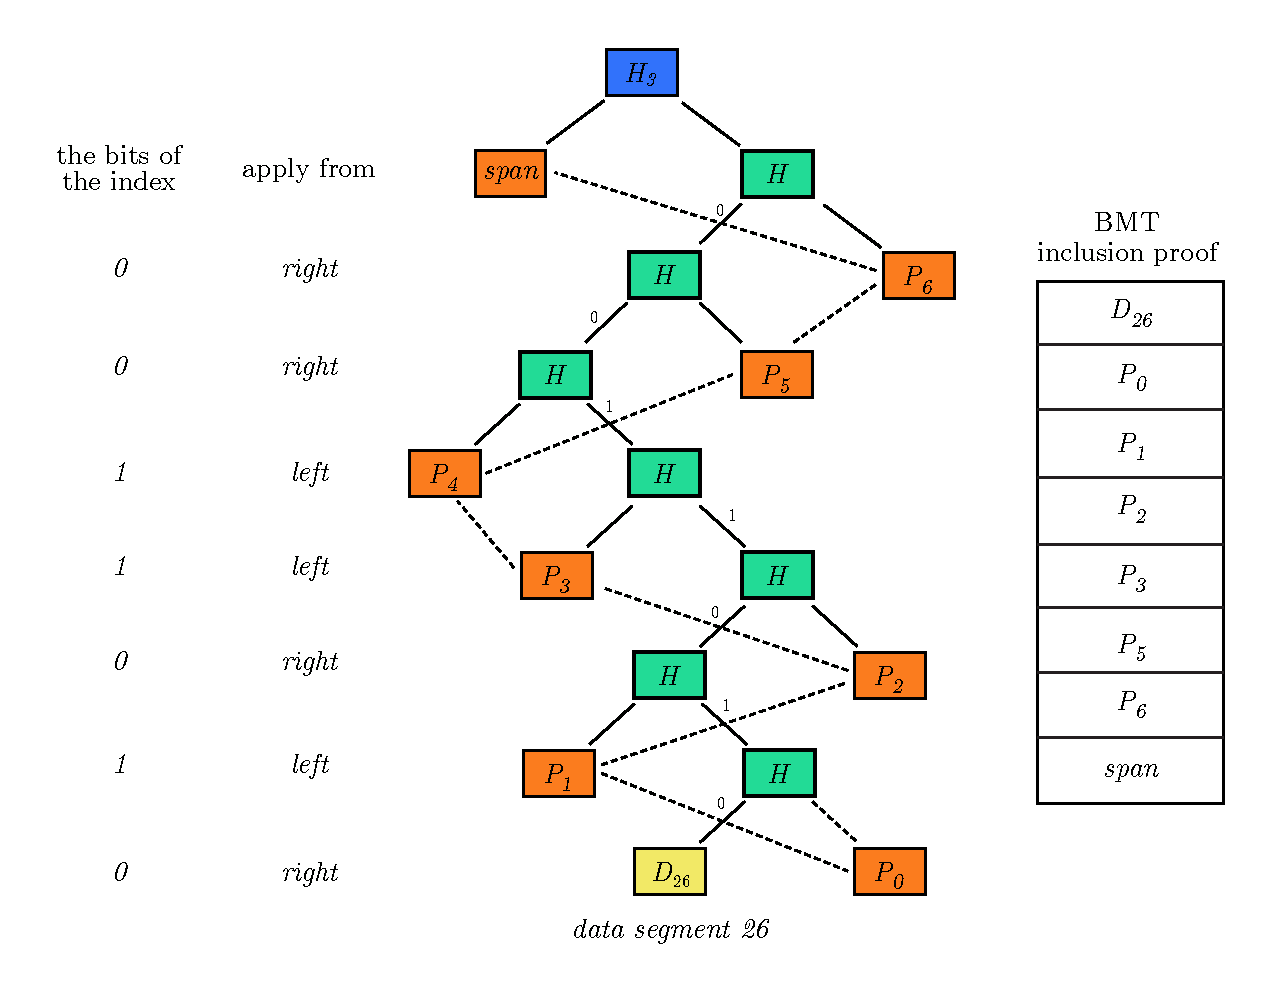
\includegraphics[width=.85\textwidth]{fig/inclusion-proof.pdf}
\caption[Compact segment inclusion proofs for chunks ]{Compact segment inclusion proofs for chunks. Assume we need proof for segment 26 of a chunk (yellow). The orange hashes of the BMT are the sister nodes on the path from the data segment up to the root and constitute what needs to be part of a proof. When these are provided together with the root hash and the segment index, the proof can be verified. The side on which proof item $i$ needs to be applied depends on the $i$-th bit (starting from least significant) of the binary representation of the index. Finally the span is prepended and the resulting hash should match the chunk root hash.}
\label{fig:chunk-inclusion}
\end{figure}

\begin{definition}[BMT segment inclusion proof \statusgreen]
\label{def:sip}
Define  $\proofof{sip}(c,i)$ as the $\mathit{BMT}$ inclusion proof on chunk $c$ for segment index $i$:
%
\begin{eqnarray}
\proofof{sip}&: &\mathit{Chunks}\times \overline{0,127} \to \mathit{SIP}\\
\mathit{SIP}&\defeq&\mathit{Segment}\times\mathit{Segment}^7\times \mathit{byte}\{8\}
\\
\proofof{sip}(c,i) &\defeq &\langle c\idx{\idx{i}},\langle h_0, h_1, \ldots, h_6\rangle, \textsc{metadata}(c)\rangle  
\end{eqnarray}
%
where
%
\begin{eqnarray}
h_j&\defeq& \mathit{BMT}(s_j,j)\\
s_j&\defeq&c\idx{\mathit{start}(i,j)\rangedel\mathit{start}(i,j)+32\cdot 2^j}
\end{eqnarray}
%
where
%
\begin{eqnarray}
\mathit{start}(i,j)&\defeq&
\begin{cases}
0 &\text{if } j=7\\
start(i,j+1) & \text{if } \mathit{int}\left(i / 2^j\right) = 0 \mod 2\\
start(i,j+1)+32\cdot 2^{j} &\text{otherwise}
\end{cases}
\end{eqnarray}
\end{definition}

In order to validate segment inclusion proofs we first introduce the prover hash function $\mathit{H}_{\Pi}$.

\begin{definition}[BMT prover function\statusgreen]
\label{def:prover-function}
%
\begin{eqnarray}
\mathit{H}_{\Pi}&:&\overline{0,127}\times\mathit{SIP}\to\mathit{Address}\\
\mathit{H}_{\Pi}(i,\langle d, sisters, m\rangle)&\defeq&\mathit{H}(m,\mathit{H}_{\Pi}^{\triangle}(7,d,sisters))
\end{eqnarray}
%
where
%
\begin{eqnarray}
\mathit{H}_{\Pi}^{\triangle}&:&\overline{0,7}\times\mathit{Segment}\times\mathit{Segment}^7\to\mathit{Address}\\
\mathit{H}_{\Pi}^{\triangle}(j,d,s)&\defeq& \begin{cases}
d & \text{ if } j=0\\
\mathit{H}(\mathit{H}_{\Pi}^{\triangle}(j-1,d,s)\concat s\idx{j-1}) & \text{if }\mathit{int}(i/2^{j-1}) = 0 \mod 2\\
\mathit{H}(s\idx{j-1}\concat \mathit{H}_{\Pi}^{\triangle}(j-1,d,s)) &\text{otherwise}
\end{cases}
\end{eqnarray}
\end{definition}


\begin{definition}[BMT SIP validation \statusgreen]
\label{def:sip-validation}
Define  $\validator{sip}(a, i, p)$ as the validator of a BMT segment inclusion proof $p$ for chunk at address $a$ on segment index $i$:
%
\begin{eqnarray}
\validator{sip}&:&\mathit{Segment}\times\overline{0,127}\times \mathit{SIP} \to \{\mathtt{T,F}\}
\\
\validator{sip}(a,i,p) &\Leftrightarrow&
\mathit{H}_{\Pi}(i,p)=a
\end{eqnarray}
\end{definition}

\begin{definition}[Single owner chunks data integrity proof \statusgreen]
\label{def:socproof}
Define a single owner chunk storage proof $\proofof{soc}(c,i)$ as a segment inclusion proof of the data payload of SOC $c$ on index $i$ together with the ID and signature of SOC $c$:
%
\begin{eqnarray}
\mathit{SIP}_\mathit{SOC} &\defeq&\mathit{SIP}\times\mathit{Sig}\times\mathit{Segment}\\
\proofof{sip[soc]} &:&\mathit{SOC}\times\overline{0,127}\to\mathit{SIP}_\mathit{SOC}\\ 
\proofof{sip[soc]}(\langle o,id,cac\rangle,i)&\defeq&  \langle p, sig, id\rangle
\end{eqnarray}
%
where
%
\begin{eqnarray}
p&=&\proofof{sip}(cac,i)\\
sig&=&\mathit{Sig}(o,id\concat \mathit{address}(cac))
\end{eqnarray}
\end{definition}

\begin{definition}[Single owner chunks data integrity validation  \statusgreen]
\label{def:socproof-validity}
Define $\validator{sip[soc]}(a, i, p)$ as the validator of a single owner chunk storage proof $p$ for chunk at address $a$ on segment index $i$:
%
\begin{eqnarray}
\validator{sip[soc]}&:&\mathit{Address}\times\overline{0,127}\times\mathit{SIP}_\mathit{SOC}\to\{\texttt{T,F}\}\\ \validator{sip[soc]}(a, i, \langle p, sig, id\rangle)&
\Leftrightarrow&a= \mathit{H}(id\concat o)
\end{eqnarray}
such that 
\begin{eqnarray}
\textsc{owner } o&=& \mathit{ECRecover}(sig,id\concat a')\\
\textsc{payload } a'&=& \mathit{H}_{\Pi}(i,p)
% \\
% \textsc{proof } p&=&\langle d, sisters, m\rangle
\end{eqnarray}
\end{definition}



\subsection{Postage stamps}
\begin{definition}[Postage stamps \statusgreen]
\label{def:postage-stamp}
%
\begin{eqnarray}
\mathit{Stamps}&\defeq& \mathit{Segment}\times\mathit{uint64}\times\mathit{Timestamp}\times\mathit{Address}\\
\mathit{ps} &=&\langle  b,i,ts,a\rangle\in \mathit{Stamps} 
\\
\textsc{batchID}(ps) &\defeq& b 
\\
\textsc{index}(ps) &\defeq &i 
\\
\textsc{timestamp}(ps)&\defeq &ts 
\\
\textsc{address}(ps) &\defeq &a 
\end{eqnarray}
\end{definition}


\begin{definition}[Storage slot reference \statusgreen]
\label{def:slot}
Define the \emph{storage slot reference} $\mathit{slot}(ps)$ of a postage stamp $ps$ as the tuple of the batch identifier and the within-batch stamp counter:
%
\begin{eqnarray}
\mathit{Slots}&\defeq&\mathit{Segment}\times\mathit{uint64}\\
\mathit{slot}&:& \mathit{Stamps}\to\mathit{Slots}\\
\mathit{slot}(ps) &\defeq &\langle \textsc{batchID}(ps),\textsc{index}(ps)\rangle 
\end{eqnarray}
%
% Naturally storage slot reference of a chunk $\mathit{slot}(c)$ is defined as the slot reference of the postage stamp attached to the chunk.
\end{definition}


\begin{definition}[Postage stamp validity \statusgreen]
\label{def:postage-stamp-validity}
Define $\validator{stamp}(ps)$ as the validator of the proof of relevance expressed as the postage stamp $ps$ relying on blockchain information:
%
\begin{eqnarray}
\validator{stamp}&:& \mathit{Stamps} \times\Gamma\times\mathit{Nodes}\to \{\mathtt{T,F}\}\\
\validator{stamp}(ps,\gamma,n) &\Leftrightarrow& \\
\textsc{authentic} & & \textsc{batchID}(ps)\in\mathrm{Batches}(\gamma)\wedge
\\
\textsc{alive} & & \mathrm{Balance}(ps) > 0 \wedge 
\\
\textsc{authorised} & &  \mathit{ECRecover}(\mathit{Sig}(ps), \mathit{encode}(ps)) = \mathrm{Owner}(ps) \wedge
\\
\textsc{available} & & 0 <= \textsc{index}(ps) < \mathrm{Size}(ps)\wedge
\\
\textsc{aligned} & & \mathit{PO}(\textsc{index}(ps),n) \geq \textsc{depth}(\mathit{reveal}(\gamma, n))
\end{eqnarray}
\end{definition}

\subsection{Ordering and sampling}


\begin{lemma}[Ordering and indexing functions\statusgreen]
\label{lem:ordering}
Given an arbitrary finite set $C$, and another set $I$ with a total order $<$.
Any invertible function total over $C$, $f: C\to I$ defines a total order $<_f$ over $C$ as follows:
%
\begin{eqnarray}
<_f&\subseteq&C\times C\\
\forall c,c'\in C, c<_f c'&\Leftrightarrow& f(c)<f(c')
\end{eqnarray}

\begin{proof}
$f$ is injective wrt $I$, so $\mathit{Image}(f)=J\subseteq I$. Since $<$ restricted to a subset ($<_J$) is also a total order over $J$.
Since $f$ is invertible, $C$ and $J$ are isomorphic and therefore the total order $<$ on $J$ carries over to $C$. \qedsymbol
\end{proof}
\end{lemma}

\begin{corollary}[hash orders\statusgreen]
Any hash function defines a total order on a finite set of byte slices.
%
\begin{proof}
The collision free nature of the hash function makes it practically invertible. The actual hashes when read as binary encodings of integers, offer a natural integer ordering over the values. 
\end{proof}

Example: the prefixed BMT hash transform (see \ref{def:prefixed-hash}) defines a total order over a set of chunks.
\end{corollary}

\begin{definition}[Sampler function]
\label{def:sampler}
%
Using $f$ and its derivative ordering on $C\subseteq\mathit{Dom}(f)$ we represent $C$ as an ordered sequence:
%
\begin{eqnarray}
\overrightarrow{\mathit{Seq}}
&:&(T\to  T)\times\mathcal{P}(T)\to T{*}\\
\overrightarrow{\mathit{Seq}}(f,C) 
&\defeq& C'\\
\text{such that }
f(C'\idx{i})<f(C'\idx{j}) &&\text{ for every } 0\leq i<j<\lvert C\rvert
\end{eqnarray}


Finally, we define a sampler function for any $f$ invertible with an image having a total order and $C\subseteq\mathit{Dom}(f)$ such that it selects a prefix slice of length $l$ from the ordered $C$:         

\begin{eqnarray}
\mathit{Sampler} &:&(T\to  T)\times\mathcal{P}(T)\times \mathit{uint64}\to T{+}\\
% \mathit{Sampler}(f,C) &:&\overline{0,\lvert C\rvert-1}\to T\{,\lvert C\rvert\}\\
\mathit{Sampler}(f,C,l) &\defeq& \overrightarrow{\mathit{Seq}}(f,C)\idx{\rangedel l}
\end{eqnarray}
\end{definition}

\section{Redistribution game}\label{sec:appendix-game}
\label{sec:redistribution-game}

\begin{definition}[Redistribution game round\statusgreen]

\label{def:redistribution-game-round} 
Define $\gamma$ as a redistribution game round.  $\gamma$ is conceived of as a multidimensional index:
%
\begin{eqnarray}
\Gamma&\defeq&\mathit{uint64}\times\mathit{uint64}\times\mathit{uint64}\\
\gamma\in\Gamma&=&\langle c,\sigma,i\rangle\\
\textsc{chain}(\gamma)&c&\text{ID of the blockchain context}\\
\textsc{series}(\gamma)&\sigma&\text{index of the parallel series}\\
\textsc{round}(\gamma)&i&\text{sequential index of the round}
\end{eqnarray}

Define $\textsc{block}(\gamma)$ as the starting block height of this particular game $\gamma$:
%
\begin{eqnarray}
\textsc{block}(\gamma)&\defeq&\textsc{round}(\gamma)\cdot \mathtt{ROUND\_LENGTH}+\mathtt{START\_BLOCK}
\end{eqnarray}

Ordering by sequential index defines the chain of games, which lets us define the $\mathit{Prev}$ function:
%
\begin{eqnarray}
\mathit{Prev}&:&\Gamma\to\Gamma\\
\mathit{Prev}(\langle c,\sigma,i\rangle)&\defeq&\langle c,\sigma,i-1\rangle
\end{eqnarray}
\end{definition}

\subsection{Transactions and on-chain registers}

The smart contract receives transactions from applicants in phases. The following virtual registers capture the information given in these transactions that are relevant for defining the winner:
\begin{itemize}[noitemsep]
\item[--] batches (see definition \ref{def:postage-stamp-validity})
\item[--] stakes (see definition \ref{def:stakes})
\item[--] commits (see definition \ref{def:commits})
\item[--] reveals (see definition \ref{def:reveals})
\end{itemize}

\begin{definition}[Stakes \statusgreen]
\label{def:stakes}
We define $\mathit{Stakes}$ as the registry of stakes resulting from transactions sent to the staking contract. A record is a tuple of a node overlay, the stake balance and the committed stake and can be updated.  
%
\begin{eqnarray}
\mathit{Stakes}&:&\Gamma\to\mathit{Nodes}\times\mathit{uint64}\times\mathit{uint64}\\
\langle n, s, m\rangle\in\mathit{Stakes}(\gamma)&\Leftrightarrow& \\
\textsc{right age}&&\exists b'<b-\mathtt{MIN\_STAKE\_AGE}, \tau\in\mathrm{Transactions}(b') \\
\textsc{node overlay}&& n = \mathit{H}(\mathrm{origin}(\tau)\concat\mathtt{BZZ\_NETWORK\_ID}\concat\mathrm{data}(\tau)\idx{0})\\
\textsc{stake balance}&& s=\mathrm{amount}(\tau)\\
\textsc{committed stake}&& m=\mathrm{data}(\tau)\idx{1}
\end{eqnarray}
%
There is only one stake allowed per node, so we can define the staked amount belonging to a node as the minumum of the stake balance and the committed stake times the unit price of storage:
% 
\begin{eqnarray}
\mathit{Stake}&:&\Gamma\times\mathit{Nodes}\to\mathit{uint64}\\
\mathit{Stake}(\gamma,n)&\defeq&\mathit{min}(s,m\cdot \mathit{Price}(\gamma))
\end{eqnarray}
%
\end{definition}

\begin{definition}[Commits \statusgreen]
\label{def:commits}
We define $\mathit{Commits}(\gamma)$ as the registry of applications for a game $\gamma$ resulting from a transaction sent to the game contract's \emph{commit} endpoint. A tuple of the overlay of the committing node, its commitment hash and the number of the block containing the transaction is entered in the register after verifying that (i) the transaction was sent during the commit phase (right time), and (ii) that the node has enough stake and is not frozen (right amount).                    
%
\begin{eqnarray}
\mathit{Commits}&:&\Gamma\to\mathit{Nodes}\times\mathit{Segment}\times\mathit{Blocks}\\
\langle n,h,b\rangle\in\mathit{Commits}(\gamma)&\Leftrightarrow&%\text{$n$ submitted $h$ as their commit}
\\
% &&\text{during the commit phase}\\
\textsc{right time}
&&b < \mathtt{PHASE\_LENGTH} \mod \mathtt{ROUND\_LENGTH} \\
\textsc{right amount}&&\mathit{stake}(\gamma,n)\geq \texttt{MINIMUM\_STAKE}\\
(\textsc{redundancy})&&
\end{eqnarray}
\end{definition}

\begin{definition}[Reveals\statusgreen]
\label{def:reveals}
We define $\mathit{Reveals}$ as the registry of reveals resulting from a transaction sent to the game contract's reveal endpoint. The reveal record is a tuple of the node overlay, the two commitment hashes, the self-reported storage depth, a serial index used for sorting, the obfuscation key, and the block number. The record is entered in the register after it is validated that (i) it was submitted during the reveal phase (right time), (ii) the commitments when obfuscated match the commit by the same node (right reveal), and (iii) that the neighbourhood selection anchor falls within the node's area of responsibility using the self-reported depth (right location). 
%
\begin{eqnarray}
\mathit{RevealEntry}&:&\mathit{Nodes}\times\mathit{Address}^2\times\mathit{uint8}^2\times\mathit{Nonce}\times\mathit{Blocks}\\
\mathit{Reveals}&:&\Gamma\to\mathcal{P}(\mathit{RevealEntry})\\
r=\langle n,chc,chs,sd,i,k,b\rangle\in\mathit{Reveals}(\gamma)&\Leftrightarrow& 
% \text{ $n$ reveals $chc, chs, sd$  as their commitment}\\
\langle\\
\textsc{node}(r)&=&n\\
\textsc{chc}(r)&=&chc\\
\textsc{chs}(r)&=&chs\\
\textsc{depth}(r)&=&sd\\
\textsc{index}(r)&=&i\\
\textsc{nonce}(r)&=&k\\
\textsc{block}(r)&=&b\\
&&\rangle\\
&\Leftrightarrow&\\
\textsc{right time}
&&p \leq b < 2p \mod r\\
&& p = \mathtt{PHASE\_LENGTH}, r= \mathtt{ROUND\_LENGTH} \\
\textsc{right reveal}&&\mathit{H}(n\concat sd\concat chc\concat chs\concat k)=h \text{ such that }\\
&&\langle n,h,b'\rangle\in\mathit{Commits}(\gamma)\text{ for some }b'\\
\textsc{right location}&&\mathit{PO}(\mathit{addr}(n),\mathit{NSA}(\mathit{Prev}(\gamma)))\geq sd\\
(\textsc{responsibility})&&
\end{eqnarray}
%
There is only one reveal allowed per node, so we can define the reveal belonging to a node:
%
\begin{eqnarray}
\mathit{Reveal}&:&\Gamma\times\mathit{Nodes}\to\mathit{RevealEntry}\\
\mathit{Reveal}(\gamma, n)&=&r
\end{eqnarray}
such that 
\begin{eqnarray}
n&=&\mathit{Node}(r)\\
r&\in&\mathit{Reveals}(\gamma)
\end{eqnarray}
\end{definition}

\subsection{Random nonces}

\begin{definition}[Random nonces for the round\statusgreen]
\label{def:nonce-round}

From the round's random seed (see definition \ref{def:random-seed} appendix \ref{sec:randomness}) we can derive all the necessary random input nonces:
%
\begin{eqnarray}
\textsc{ N.hood Selection Anchor   }\mathit{NSA}(\gamma)&\defeq&\mathit{H}(\mathcal{R}(\gamma)\concat BE^{64}(\mathit{SK}(\gamma)))\\
\textsc{ Truth Selection Nonces  }\mathit{TSN}(\gamma)&\defeq&\mathit{H}(\mathcal{R}(\gamma)\concat\mathit{BE}^{8}(0)) \\
\textsc{ Winner Selection Nonces  }\mathit{WSN}(\gamma, i)&\defeq&\mathit{H}(\mathcal{R}(\gamma)\concat\mathit{BE}^{8}(1)) \\
\textsc{ Reserve sampling salt } \mathit{RSS}(\gamma)&\defeq&\mathit{H}(\mathcal{R}(\gamma)) \\
\textsc{ Segment Selection Nonce } \mathit{SSN}(\gamma,i)&\defeq&\mathit{H}(\mathcal{R}(\gamma)\concat\mathit{BE}^{8}(i))
\end{eqnarray}
where 
\begin{eqnarray}
\mathit{SK}&:&\Gamma\to\mathit{uint64}\\
\mathit{SK}(\gamma)&\defeq&\begin{cases}0&\text{if }\lvert\mathit{Reveals}(\gamma)\rvert>0\\
\mathit{SK}(\mathit{Prev}(\gamma))+1&\text{otherwise}
\end{cases}
\end{eqnarray}

Let us now define the witness selection function $\mathcal{W}$ that selects two random witness indexes as well as the last index of the reserve sample such that they are all distinct:
%
\begin{eqnarray}
\mathcal{W}&:&\Gamma\times\mathit{uint64}\times\{0,1,2\}\to\mathit{uint8}\\
\mathcal{W}(\gamma,m,k)&\defeq&\begin{cases}
\mathit{SSN}(\gamma,0) \mod m-1&\text{ if }k=0\\
m-1&\text{ if }k=2\\
m-2&\text{ if }k=1 \land\\
& \mathit{SSN}(\gamma,0)=\mathit{SSN}(\gamma,1) \mod m-1\\
\mathit{SSN}(\gamma,1) \mod m-2&\text{ otherwise }
\end{cases}
\end{eqnarray}
\end{definition}

% \subsection{Reserve Size}

% \begin{definition}[Network reserve size]
% \label{def:reserve-size}
% Define $\mathrm{ReserveSize}(\gamma)$, the network reserved capacity as the total number of storage slots by all batches valid at block $\mathit{Block}(\gamma)$. This can be read from the batch registry contract:
% %
% \begin{eqnarray}
% \mathrm{ReserveSize}&:&\Gamma\to \mathit{uint64}\\
% \mathrm{ReserveSize}(\gamma)&\defeq&\Sigma_{b\in \mathit{Batches}(\gamma)}\mathrm{Size}(b,\gamma)
% \end{eqnarray}
% \end{definition}


% \begin{definition}[Reserve depth]
% \label{def:reserve-depth}
% Define $\mathrm{ReserveDepth}(\gamma)$ as the base 2 log of the number of neighbourhoods needed to provide redundant storage for the volume of chunks corresponding to the network reserve size at block $\mathit{Block}(\gamma)$ given a fixed node storage capacity of depth \texttt{NODE\_RESERVE\_DEPTH}:
% %
% \begin{eqnarray}
% \mathrm{ReserveDepth}&:&\Gamma\to \mathit{uint8}\\
% \mathrm{ReserveDepth}(\gamma)&\defeq&\mathit{int}(\mathit{log}_2(\mathrm{ReserveSize}(\gamma)))-\texttt{NODE\_RESERVE\_DEPTH}
% \end{eqnarray}
% \end{definition}


\subsection{Winner selection and claim validation}

\begin{definition}[Prefixed hash \statusgreen]
\label{def:prefixed-hash}
Define the hash prefixing function $\mathit{prefix}(H,p)$ as a function which when applied to a hash function $\mathit{H}$ and a constant byte slice $p$  outputs a hash function which for every input returns the hash of the input prefixed by $p$ using $H$.
%
\begin{eqnarray}
\mathit{prefix}&: &(\mathit{byte}{*}\to\mathit{Segment})\times\mathit{byte}{*}\to (\mathit{byte}{*}\to\mathit{Segment})
\\
\mathit{prefix}(H,p) &: &\mathit{byte}{*}\to\mathit{Segment}\\
\mathit{prefix}(H,p)(b) &\defeq & H(p\concat b)
\end{eqnarray}

Exceptionally, we define the prefixed version of BMT hash (denoted as $\mathit{BMT}[]$) as one   that uses the prefixed verson of its base hash:
%   
\begin{eqnarray}
\mathit{BMT}[]&: &\mathit{byte}{*}\to\mathit{Chunk}\times\mathit{byte}\{8\}\to\mathit{Segment}\\
\mathit{BMT}[p]&\defeq&\mathit{BMT}[\mathit{prefix}(\mathit{H},p)]
\end{eqnarray}

\end{definition}
    
\begin{definition}[Transformed chunk reserve sample\statusgreen]
\label{def:transformed-reserve}
%
Let us now define the chunk transformation function $\Delta^C(p)$
for a random nonce prefix $p$ as follows: 
%
\begin{eqnarray}
\Delta^C&:&\mathit{Nonce}\to\mathit{Chunks}\to\mathit{Segment}\\
\Delta^C(p)&:&\mathit{Chunks}\to\mathit{Segment}\\
\Delta^C(p)(c)&\defeq&\mathit{BMT}[p](\textsc{data}(c),\textsc{metadata}(c))
\end{eqnarray}
%
Define the transformed reserve sample $\mathit{RS^C}(\gamma,n)$ for game $\gamma$ and node $n$ as the first  $2^d$ chunks of the node's reserve at block $\textsc{block}(\gamma)$, using the ordering defined (see lemma \ref{lem:ordering} and definition \ref{def:sampler}) by the hash (see definition \ref{def:prefixed-hash}) of their data  using BMT with 256-bit Keccak prefixed with random nonce $p$ as its base hash.
%
\begin{eqnarray}
\mathit{RS^C}&:&\Gamma\times\mathit{Nodes}\to\mathit{Chunks}{*}\\\
\mathit{RS^C}(\gamma,n)&\defeq&\mathit{Sampler}(\Delta^C(p),\mathit{Reserve}(\gamma,n),2^d)
\end{eqnarray}
where 
\begin{eqnarray}
d & = & \texttt{SAMPLE\_DEPTH} \text{ (see \ref{sec:constants})} \\
p & = & \mathit{RSS}(\gamma) \text{ (see definition \ref{def:nonce-round})}
\end{eqnarray}
\end{definition}


\begin{definition}[Chunk reserve sample commitment hash \statusgreen]
\label{def:chc}
Define $\mathit{CH^C}(\gamma,n,)$ for game $\gamma$ and node $n$ as the BMT chunk hash of the packed address chunk (see definition \ref{def:pac}) packing the chunks of the transformed reserve sample (see definition \ref{def:transformed-reserve}) for game $\gamma$ and node $n$.
%
\begin{eqnarray}
\mathit{CH^C}&:&\Gamma\times\mathit{Nodes}\to\mathit{Address}\\
\mathit{CH^C}(\gamma,n)&\defeq&\mathit{Address}(\mathit{PAC^C}(\mathit{RS^C}(\gamma, n), p))
    \end{eqnarray}
where
\begin{eqnarray}
p & = & \mathit{RSS}(\gamma) \text{ (see definition \ref{def:nonce-round})}
\end{eqnarray}
and where 
\begin{eqnarray}
\mathit{PAC^C}&:&\mathit{Chunks}{*}\times\mathit{Nonce}\to\mathit{Chunks}\\
\mathit{PAC^C}(C,p)&\defeq&\mathit{CAC}{}\left(\Concat_{i=0}^{\mathit{len}(C)-1} \mathit{Seg}(C\idx{i},p), m\right)
\end{eqnarray}
where
\begin{eqnarray}
\mathit{Seg}(C\idx{i},p) &=& \mathit{Address}(C\idx{i})\concat \Delta^C(p)(C\idx{i}) \\
m & = & \mathit{LE}^{64}(2\cdot32\cdot\mathit{len}(C))
\end{eqnarray}
\end{definition}

\begin{definition}[Transformed slots reserve sample\statusgreen]
\label{def:transformed-slots}
%
Let us now define the slots transformation function $\Delta^S(p)$
for a random nonce $p$ as follows: 
%
\begin{eqnarray}
\Delta^S&:&\mathit{Nonce}\to\mathit{Chunks}\to\mathit{Segment}\\
\Delta^S(p)&:&\mathit{Chunks}\to\mathit{Segment}\\
\Delta^S(p)(c)&\defeq&\mathit{H}[p](\mathit{Slot}(\mathit{Stamp}(c)))
\end{eqnarray}
%
Define the transformed reserve sample $\mathit{RS^S}(\gamma,n)$ for game $\gamma$ and node $n$ as the first $2^d$ chunks  of the node's reserve at block $\textsc{block}(\gamma)$, using the ordering defined by the slot transformation function using prefix $p$:%
\begin{eqnarray}
\mathit{RS^S}&:&\Gamma\times\mathit{Nodes}\to\mathit{Chunks}{*}\\\
\mathit{RS^S}(\gamma,n)&\defeq&\mathit{Sampler}(\Delta^S(p),\mathit{Reserve}(\gamma,n),2^d)
\end{eqnarray}
where 
\begin{eqnarray}
d & = & \texttt{SAMPLE\_DEPTH} \text{ (see \ref{sec:constants})} \\
p & = & \mathit{RSS}(\gamma) \text{ (see definition \ref{def:nonce-round})}
\end{eqnarray}
\end{definition}


\begin{definition}[Transformed slots reserve sample commitment hash \statusgreen]
\label{def:chs}
Define $\mathit{CH^S}(\gamma,n)$ for game $\gamma$ and node $n$ as the BMT chunk hash of the packed address chunk (see definition \ref{def:pac}) the chunks of the transformed reserve sample (see definition \ref{def:transformed-reserve}) for game $\gamma$ and node $n$.
%
\begin{eqnarray}
\mathit{CH^S}&:&\Gamma\times\mathit{Nodes}\to\mathit{Address}\\
\mathit{CH^S}(\gamma,n)&\defeq&\mathit{Address}(\mathit{PAC}(\mathit{RS^S}(\gamma, n),m))
\end{eqnarray}
where
\begin{eqnarray}
m & = & \mathit{LE}^{64}(32\cdot 2^d)\\
d & = & \texttt{SAMPLE\_DEPTH} \text{ (see \ref{sec:constants})} 
\end{eqnarray}
\end{definition}

\begin{definition}[Weighted selection\statusgreen]
\label{def:weighted-selection}
We define $\mathit{WeightedSelect}(w,k)$ as a sampler function which selects an index $0<i<\mathit{len}(w)$ such that the indexes have a probability of being selected according to the weights in $w$ determined by the input nonce (pseudorandom number) $k$.
%
\begin{eqnarray}
\mathit{WeightedSelect}&:&\mathit{uint256}{+}\times\mathit{uint256}\to\mathit{uint256}{+}\\
\mathit{WeightedSelect}(w,k)&\defeq&
\begin{cases}
    i&\text{if }k <w\idx{i}\mod W\idx{i}\\
\mathit{WeightedSelect}(w\idx{\rangedel i},k)&
\text{otherwise}
\end{cases}
\end{eqnarray}
such that $i=\mathit{len}(w)-1$,   
and
where $W$ (cumulative weights) is defined as
\begin{eqnarray}
W & : & \mathit{uint256}{+}\to\mathit{uint256}\\
W\idx{i} &\defeq & \begin{cases}
    w\idx{0}&\text{if }i=0\\
    W\idx{i-1}+w\idx{i}&\text{otherwise}
\end{cases} 
\end{eqnarray}
\end{definition}



\begin{definition}[Truth selection\statusgreen]
\label{def:truth-selection}
We determine the truth from reveals through selection weighted by stake density using the truth selection nonce as random input. 
\begin{eqnarray}
\mathit{Truth}&:& \Gamma\to\mathit{RevealEntry}\\
\mathit{Truth}(\gamma)&\defeq&\mathit{R}(\gamma)\idx{\mathit{WeightedSelect}(\mathit{weights},\mathit{TSN}(\gamma))}
\end{eqnarray}
where weights are stake densities such that 
\begin{eqnarray}
\mathit{weights}\idx{i}&=&\mathit{Stake}(\gamma,\textsc{node}(R\idx{i}))\cdot 2^{\textsc{depth}(R\idx{i})}
\end{eqnarray}
where $R$ is the reveals of the round sorted by index:
\begin{eqnarray}
R&=&\overrightarrow{\mathit{Seq}}(\textsc{index},\mathit{Reveals}(\gamma))
\end{eqnarray}
\end{definition}

\begin{definition}[Honest reveals\statusgreen]
We define honest reveals as the subset of reveals for the round agreeing with the truth in reserve commitment hashes and storage depth.
\label{def:honest-reveals}
\begin{eqnarray}
\mathit{HonestReveals}&:&\Gamma\to\mathit{RevealEntry}{*}\\
\mathit{HonestReveals}(\gamma)&\defeq&\overrightarrow{\mathit{Seq}}(\textsc{index},\{r\in\mathit{Reveals}(\gamma)|\mathit{Honest}(r)\})
\end{eqnarray}
where
\begin{eqnarray}
\mathit{Honest}&:&\mathit{RevealEntry}\to\{\texttt{T,F}\}\\
\mathit{Honest}(r)&\leftrightarrow&\\
&&\textsc{chc}(r)=\textsc{chc}(\mathit{truth}(\gamma))\ \land\\
&&\textsc{chs}(r)=\textsc{chs}(\mathit{truth}(\gamma))\ \land\\
&&\textsc{depth}(r)=\textsc{depth}(\mathit{truth}(\gamma))
\end{eqnarray}
\end{definition}

\begin{definition}[Winner selection\statusgreen]
\label{def:winner-selection}
We determine the winner from honest reveals through selection weighted by stake using the winner selection nonce as random input. 
\begin{eqnarray}
\mathit{Winner}&:& \Gamma\to\mathit{RevealEntry}\\
\mathit{Winner}(\gamma)&\defeq&\mathit{HonestReveals}(\gamma)\idx{\mathit{WeightedSelect}(\mathit{weights},\mathit{WSN}(\gamma))}
\end{eqnarray}
where weights are stakes such that 
\begin{eqnarray}
\mathit{weights}\idx{i}&=&\mathit{Stake}(\gamma,\textsc{node}(\mathit{HonestReveals}\idx{i}))
\end{eqnarray}
\end{definition}

\subsection{Proofs of reserve}
\label{sec:proofs}
    
\begin{definition}[Proof of reserve \statusgreen]
\label{def:por}
Proof of reserve provides evidence that the reserve is replicating relevant content and shows a proof of recency of retaining chunk data in full integrity.
%
\begin{eqnarray}
\mathit{POR}&:&\mathit{SIP}^2\times\mathit{Stamps}\\
\proofof{r}&:&\Gamma\times\mathit{Chunks}\times\mathit{Chunks}{+}\times\{0,1,2\}\to\mathit{POR}\\
\proofof{r}(\gamma,c,C,k)&\defeq&\langle\\
\textsc{witness proof}&&\proofof{sip}(c,d\cdot i), \\
\textsc{retention proof}&&\proofof{sip}(C\idx{i},j), \\
\textsc{postage stamp}&&\mathit{Stamp}(C\idx{i})\\
&&\rangle
\end{eqnarray}
where 
\begin{eqnarray}
i&=&\mathcal{W}(\gamma,\mathit{len}(C),k)\\
j&=& \mathit{SSN}(\gamma,k)\mod 128\\
d &=&\frac{\mathit{SegCnt}(c)}{\mathit{len}(C)} \left(=\begin{cases}
    1& \text{if } C=RS^S\\
2 &\text{if } C=RS^C
\end{cases}
\right)
\end{eqnarray}
\end{definition}


\begin{definition}[Proof of reserve validation\statusgreen]
\label{def:por-validation}
%
\begin{eqnarray}
\validator{r}&:&\Gamma\times\mathit{Nodes}\times\mathit{Address}\times\{0,1,2\}\times\mathit{POR}\to\{\texttt{T,F}\}\\
\validator{r}(\gamma, n, ch, k, \pi)&\leftrightarrow& \\
\textsc{relevance}&&\validator{sip}(ch,d\cdot i,p_w)\land\\
    && \validator{stamp}(ps, \gamma, n) \land\\
\textsc{retention}&& \textsc{data}(p_w)=a\land\\
    && \validator{sip}(a,j,p_r)\land\\
\textsc{recency}&&i=\mathcal{W}(\gamma,\mathit{SegCnt}(p_w),k)\land\\
    &&j = \mathit{SSN}(\gamma,k)\mod 128\land\\
\textsc{retrievability}&&\mathit{PO}(a,n) \geq sd 
\end{eqnarray}
where
\begin{eqnarray}
a&=& \textsc{Address}(ps)\\
\pi&=&\langle p_w, p_r, ps\rangle\\
sd &=& \textsc{depth}(\mathit{Reveal}(\gamma, n))\\
d&=&\frac{\mathit{SegCnt}(p_w)}{2^D}\left(=\begin{cases}
    1& \text{if } C=RS^S\\
2 &\text{if } C=RS^C
\end{cases}\right)\\
D& =& \texttt{SAMPLE\_DEPTH} \text{ (see \ref{sec:constants})}
\end{eqnarray}
\end{definition}


\begin{definition}[Proof of chunk density validation\statusgreen]
\label{def:chunk-density-validition}
%
Define $\validator{cd}(\gamma, p_0,p_1,p_2)$ as the validation function for the proof of chunk density for round $\gamma$ and proof of reserve and segment inclusion proof pairs $p_0,p_1,p_2$.
%
\begin{eqnarray}
\mathit{PORT}&:&\mathit{POR}\times\mathit{SIP}\\
\validator{cd}&:&\Gamma\times\mathit{PORT}^3\to\{\texttt{T,F}\}\\
\validator{cd}(\gamma, \pi_0,\pi_1,\pi_2)&\leftrightarrow&\\
\textsc{right data segment}&&   \textsc{data}(pr_k)= \textsc{data}(pt_k)\text{ for }k\in\{0,1,2\}\land\\
\textsc{right address}&& \textsc{sister}(pw_k,0)=ta_k\text{ for }k\in\{0,1,2\}\land\\
\textsc{right order}&& ta_0<ta_1<ta_2\land\\
\textsc{right size}&& ta_2\leq\texttt{MAX\_SAMPLE\_VALUE}
\end{eqnarray}
where  for $k\in\{0,1,2\}$
\begin{eqnarray}
ta_k& = & \mathit{H}_{\Pi}(p,j_k,pt_k)\\
j_k& = &\mathit{SSN}(\gamma,k)\mod 128\\
\pi_k&=& \langle\langle pw_k, pr_k, \_\rangle, pt_k\rangle
% \\
% w_k&=&\langle O+i_k,ta_k\rangle
\end{eqnarray}
and where
\begin{eqnarray}
p & = & \mathit{RSS}(\mathit{Prev}(\gamma)) \text{ (see definition \ref{def:nonce-round})}
% D& =& \texttt{NODE\_RESERVE\_DEPTH} \text{ (see \ref{sec:constants})}
\end{eqnarray}
\end{definition}

\begin{definition}[Proof of stamp density validation\statusgreen]
\label{def:stamp-density-validition}
%
Define $\validator{sd}(\gamma, ps_0,ps_1,ps_2)$ as the validation function for the proof of stamp density for round $\gamma$ and postage stamps $ps_0,ps_1,ps_2$.
%
\begin{eqnarray}
\validator{sd}&:&\Gamma\times\mathit{Stamps}^3\to\{\texttt{T,F}\}\\
\validator{sd}(\gamma, ps_0,ps_1,ps_2)&\leftrightarrow &\\ 
\textsc{right order}&& ta_0<ta_1<ta_2\land\\
\textsc{right size}&& ta_2\leq\texttt{MAX\_SAMPLE\_VALUE}
\end{eqnarray}
where for $k\in\{0,1,2\}$
\begin{eqnarray}
ta_k& =& \mathit{H}(\mathit{Slot}(ps_k)\concat p)
\end{eqnarray}
and where
\begin{eqnarray}
p & = & \mathit{RSS}(\mathit{Prev}(\gamma)) \text{ (see definition \ref{def:nonce-round})}
\end{eqnarray}
\end{definition}

% \newpage
\begin{definition}[Proof of entitlement\statusgreen]
\label{def:poe}
Proof of entitlement captures all the evidence a node needs to submit with their claim transaction to valildate. 
%
\begin{eqnarray}
\mathit{POE}&:&\mathit{PORT}^3\times\mathit{POR}^3\\
\proofof{ent}&:&\Gamma\times\mathit{Nodes}\to\mathit{POE}\\
\proofof{ent}(\gamma,n)&\defeq&\langle\\
&&\langle\proofof{por}(\gamma,n,\mathit{PAC^C}(crs,p), crs,0),pt_0\rangle,\\
&&\langle\proofof{por}(\gamma,n,\mathit{PAC^C}(crs,p),crs,1),pt_1\rangle,\\
&&\langle\proofof{por}(\gamma,n,\mathit{PAC^C}(crs,p),crs,2),pt_2\rangle,\\
&&\proofof{por}(\gamma,n,\mathit{PAC}(srs),srs,0),\\
&&\proofof{por}(\gamma,n,\mathit{PAC}(srs),srs,1),\\
&&\proofof{por}(\gamma,n,\mathit{PAC}(srs),srs,2),\\
&&\rangle
\end{eqnarray}
where for $k\in\{0,1,2\}$
\begin{eqnarray}
pt_k&=& {\proofof{sip}_\mathit{prefix}}(p,r\idx{i_k},j_k)\\
j_k & = & \mathit{SSN}(\gamma,k)\mod 128\\
i_k & = & \mathcal{W}(\gamma,\mathit{length}(crs),k)
\end{eqnarray}
and where 
\begin{eqnarray}
crs& = & \mathit{RS^C}(\gamma, n)\\
srs & = & \mathit{RS^S}(\gamma, n)\\
p & = & \mathit{RSS}(\mathit{Prev}(\gamma)) \text{ (see definition \ref{def:nonce-round})}
\end{eqnarray}
\end{definition}




\begin{definition}[Winner's claim validation\statusgreen]
\label{def:claim-validation}
%
Define $\validator{poe}(\gamma, p)$ as the validation function for the proof of entitlement $p$ as part of the winning claim for game $\gamma$:
%
\begin{eqnarray}
\validator{poe}&:&\Gamma\times\mathit{POE}\to\{\texttt{T,F}\}\\
\validator{poe}(\gamma, p) &\Leftrightarrow\\
%
\textsc{reserve:\ \ \ \ \ \ \ \ \ \ \ \ \ \ }\\
\textsc{chunks}
&&\forall k\in\{0,1,2\},\validator{r}(\gamma,n,\textsc{chc}(r),k,\pi_k)\land\\
\textsc{stamps}
&&\forall k\in\{0,1,2\}, \validator{r}(\gamma,n,\textsc{chs}(r),k,\phi_k)\land\\
\textsc{reserve size:\ \ \ \ \ \ \ }\\
\textsc{chunk density}&&\validator{cd}(\gamma, \langle \pi_0,pt_0\rangle, \langle \pi_1,pt_1\rangle, \langle \pi_2,pt_2\rangle)\land\\
%
\textsc{stamp density}&&
\validator{sd}(\gamma,\textsc{ps}(\phi_0),\textsc{ps}(\phi_1),\textsc{ps}(\phi_2))
\end{eqnarray}
where
\begin{eqnarray}
n&=& \textsc{node}(r)\\
r&=& \mathit{Winner}(\gamma)\\
p &= &\langle\langle \pi_0,pt_0\rangle, \langle \pi_1,pt_1\rangle,\langle \pi_2,pt_2\rangle,\phi_0,\phi_1,\phi_2\rangle
\end{eqnarray}
\end{definition}

% \textsc{redundancy}&& \mathit{Stake}(\gamma, n)\geq \texttt{MINIMUM\_STAKE} \land\\
% \textsc{responsibility}&& \mathit{PO}(\mathit{addr}(n),\mathit{NSA}(\gamma))\geq sd \land\\


\begin{corollary}[Outpayment scheme is fair]
Rewarding the pot to randomly selected neighbourhood implements a  redistribution scheme that is fair across neighbourhoods.
\begin{proof}
With the consensus mechanism we can show that the Nash-optimal strategy of nodes is to follow the protocol and consent on the reserve. On the other hand, the optimal strategy for uploaders is to uniformly distribute chunks across the name space. As a consequence, nodes are expected to have identical storage depth and its variance is independent of being chosen. Long term then relative cumulative outpayments by the redistribution game converge to the fair share.
\end{proof}

Secondly, we argue that the mode of selecting the winner is fair within neighbourhoods. 
\begin{proof}
    
\end{proof}
\end{corollary}



\chapter{Data types and algorithms}\label{spec:convention}

\orange{}

\section{Built-in primitives \statusyellow}\label{spec:format:builtin}
\subsection{Crypto \statusgreen}\label{spec:format:crypto}

This section describes the crypto primitives used throughout the specification. They  are exposed as  buzz built-in  functions.
The modules are hashing, random number generation, key derivation, symmetric and asymmetric encryption (ECIES), mining (i.e., finding a nonce), elliptic curve key generation, digital signature (ECDSA), Diffie--Hellman shared secret (ECDH) and Reed-Solomon  (RS) erasure coding.

Some of the built-in crypto primitives (notably, sha3 hash, and ECDSA ecrecover) are replicating crypto functionality of the Ethereum VM. These are defined here with the help of ethereum api calls to a smart contract. This smart contract just implements the primitives of "buzz" and only has read methods.

\subsubsection{Hashing}

The base hash function implements Keccak256 hash as used in Ethereum.

\begin{definition}[Hashing]\label{def:hash}
\begin{lstlisting}[language=buzz1]
// /crypto

define function hash @input []byte
    ?and/with @suff
    return segment
as
    ethereum/call "sha3" with @input append= @suff
         on context contracts "buzz" 
\end{lstlisting}
\end{definition}  


\subsubsection{Random number generation}

\begin{definition}[Random number generation]\label{def:rng}
\begin{lstlisting}[language=buzz1]
// /crypto

define function random type 
    return [@type size]byte 

\end{lstlisting}
\end{definition}    


\subsubsection{Scrypt key derivation}

The crypto key derivation function implements \lstinline{scrypt} 
% \cite{percival2009stronger}.

\begin{definition}[Scrypt key derivation]\label{def:scrypt}
\begin{lstlisting}[language=buzz1]
// /crypto

define type salt as [segment size]byte

define type key as [segment size]byte

// params for scrypt key derivation function
// scrypt.key(password, salt, n, r, p, 32) to generate key

define type kdf
    n int // 262144
    r int // 8
    p int // 1

define function scrypt from @password
    with   salt 
    using  kdf
    return key

\end{lstlisting}
\end{definition}  

\subsubsection{Mining helper}

This module provides a very simple helper function that finds a nonce that when given as the single argument to a mining function returns true.

\begin{definition}[Mining a nonce]\label{def:mine}
\begin{lstlisting}[language=buzz1]
// /crypto

define type nonce as [segment size]byte

define function mine @f function of nonce return bool
as
    @nonce = random key
    return @nonce if call @f @nonce
    self @f
    
\end{lstlisting}
\end{definition}  

\subsubsection{Symmetric encryption}

Symmetric encryption uses a modified blockcipher with 32 byte blocksize in counter mode.
The segment keys are generated by hashing the chunk-specific encryption key with the counter and hash that again. This second step is required so that a segment can be selectively disclosed in a 3rd party provable way yet without compromising the security of the rest of the chunk.

The module provides input length preserving blockcipher encryption.

\begin{definition}[Blockcipher]\label{def:crypt}
\begin{lstlisting}[language=buzz1]
// /crypto

// two-way (en/de)crypt function for segment
define function crypt.segment segment
    with key
    at @i uint8
as
    hash @key and @i        // counter mode 
        hash                // extra hashing
        to @segment length  // chop if needed
        xor @segment        // xor key with segment

// two-way (en/de)crypt function for arbitrary length 
define function crypt @input []byte
    with key
    return [@input length]byte
as
    @segments = @input each segment size    // iterate segments of input
        go crypt.segment at @i++ with @key  // concurrent crypt on segments
    return wait for @segments               // wait for results
        join                                // join (en/de)crypted segments
        
\end{lstlisting}
\end{definition}    

\subsubsection{Elliptic curve keys}

Public key cryptography is the same as in Ethereum, it uses the secp256k1 elliptic curve.  


\begin{definition}[Elliptic curve key generation]\label{def:ec-keys}
\begin{lstlisting}[language=buzz1]
// /crypto
define type pubkey  as [64]byte
define type keypair
    privkey [32]byte
    pubkey
    
define type address as [20]byte

define function address pubkey
    return address
as 
    hash pubkey 
        from 12

define function generate 
    ?using entropy
as
    @entropy = random segment if no @entropy
    http/get "signer/generate?entropy=" append @entropy 
        as keypair

\end{lstlisting}
\end{definition}    

\subsubsection{Asymmetric encryption}

Asymmetric encryption implements ECIES based on  the secp256k1 elliptic curve. 
%  TODO: this needs more detail

\begin{definition}[Asymmetric encryption]\label{def:asymmetric-encryption}
\begin{lstlisting}[language=buzz1]
// /crypto

define function encrypt @input []byte 
    for pubkey
    return [@input length]byte

define function decrypt @input []byte 
    with keypair
    return [@input length]byte

\end{lstlisting}
\end{definition}  


\subsubsection{Signature}

Crypto's  built-in signature module implements secp2156k1 elliptic curve based ECDSA. The actual signing happens in the external signer running as a separate process (possibly within the secure enclave). As  customary  in Ethereum, the  signature is represented and serialised using the r/s/v format,

\begin{definition}[Signature]\label{def:signature}
\begin{lstlisting}[language=buzz1]
// /crypto

define type signature
    r segment
    s segment
    v uint8
    signer private keypair
    

define type doc 
    preamble []byte
    context  []byte
    asset    segment
    
define function sign @input []byte 
    by keypair
    return signature
as
    @doc = doc{ "swarm signature", context caller, @input }
    @sig = http/get "signer/sign?text=" append @doc 
        append "&account=" append @keypair pubkey address
            as signature 
    @sig signer = @keypair
    @sig
    
define function recover signature
    with @input []byte
    from @caller []byte
    return pubkey
as
    @doc =  doc{ "swarm signature", @caller, @input } as bytes
    ethereum/call "ecrecover" with 
        on context contracts "buzz" 
            as pubkey

\end{lstlisting}
\end{definition}  


\subsubsection{Diffie-Hellmann shared secret}

The shared secret module implements elliptic curve based Diffie--Helmann shared secret (ECDH) using the usual secp256k1 elliptic curve.
The actual DH comes from the external signer which is then hashed together with a salt.

\begin{definition}[Shared secret]\label{def:dh}
\begin{lstlisting}[language=buzz1]
// /crypto

define function shared.secret between keypair
    and pubkey
    using salt
    return [segment size]byte
as
    http/get "signer/dh?pubkey=" append @pubkey append "&account=" @keypair address
        hash with @salt

\end{lstlisting}
\end{definition}  

\subsubsection{Erasure coding}\label{spec:format:erasure}

Erasure coding interface provides wrappers \lstinline{extend/repair} for the encoder/decoder that work directly on a list of chunks.%
%
\footnote{Cauchy-Reed-Solomon erasure codes based on \url{https://github.com/klauspost/reedsolomon}.
}

Assuming $n$ out of $m$ coding.
\lstinline{extend} takes a list of $n$ data chunks and an argument for the number of required parities. It returns the parity chunks only.
\lstinline{repair} takes a list of $m$ chunks (extended with \emph{all} parities) and an argument for the number of parities $p=m-n$, that designate the last $p$ chunks as parity chunks. It returns the list of $n$ repaired data chunks only.
The encoder does not know which parts are invalid, so missing or invalid chunks should be set to \lstinline{nil} in the argument to repair.
If parity chunks are needed to be repaired, you call \lstinline{repair @chunks with @parities; extend with @parities}

\begin{definition}[CRS erasure code interface definition]\label{def:crs}
\begin{lstlisting}[language=buzz1]
// /crypto/crs

define function extend @chunks []chunk 
    with @parities uint
    return [@parities]chunk

define function repair @chunks []chunk   
    with @parities uint
   return [@chunks length - @parities]chunk

\end{lstlisting}
\end{definition}

\begin{definition}[CRS erasure coding parameters]\label{def:crs-params}
\begin{lstlisting}[language=buzz1]
// /crypto/crs
define strategy as "race"|"fallback"|"disabled"

define type params 
    parities uint
    strategy 
     
\end{lstlisting}
\end{definition}


\subsection{State store \statusgreen}\label{spec:format:statestore}
% \input{specs/api/statestore.tex}

\begin{definition}[State store]\label{def:state-store}
\begin{lstlisting}[language=buzz1]
// /statestore

define type key []byte
define type db  []byte
define type value []byte

define function create db

define function destroy db

define function put value
    to db
    on key
    
define function get key 
    from db
    return value
\end{lstlisting}
\end{definition}


\subsection{Local context and configuration \statusgreen}\label{spec:format:local}
% \input{specs/api/local.tex}


\begin{definition}[Context]\label{def:scontext}
\begin{lstlisting}[language=buzz1]
// /context

define type contract as "buzz"|"chequebook"|"postage"|""

define type context
    contracts [contract]ethereum/address 
\end{lstlisting}
\end{definition}

\section{Bzz address\statusgreen}\label{spec:format:bzzaddress}
\subsection{Overlay address \statusyellow}

Swarm's overlay network uses 32-byte addresses. In order to help  uniform utilisation of the address space,  these addresses must be derived using a hash function. A Swarm node must be associated a \gloss{Swarm base account} or \gloss{bzz account}, which is an Ethereum account that the node (operator) must possess the private key for. The node's overlay address is derived the public key of this account. 

\begin{definition}[Swarm overlay address of node A]\label{def:overlay}
\begin{equation}
\mathit{overlayAddress}(A) \defeq \mathit{Hash}(\mathit{ethAddress}|\mathit{bzzNetworkID})         
\end{equation}
where
\begin{itemize}
\item $\mathit{Hash}$ is the 256-bit Keccak SHA3 hash function
\item \emph{ethAddress} - the ethereum address  (bytes,  not hex) derived from the node's base account public key: $\mathit{account}\defeq\mathit{PubKey}(K_A^\mathit{bzz})[12:32]$), where
    \begin{itemize}
    \item \emph{PubKey} is the \emph{uncompressed} form of the public key of a keypair \emph{including} its $04$ (uncompressed) prefix.
    \item $K_A^\mathit{bzz}$ refers to the node's bzz account key pair
    \end{itemize}
\item \emph{bzzNetworkID} is the bzz network id of the swarm network serialised as a little-endian binary \emph{uint64}.
\end{itemize}
\end{definition}

In a way, deriving the node address from a public key means the overlay address space is not freely available: to occupy an address you must possess the private key of the address which other nodes need to verify. Such authentication is easy using a digital signature of a shared consensual piece of text, see \ref{spec:format:bzzaddress}.

\subsection{Underlay address \statusyellow}

To enable peers to locate the a node on the network, the overlay address is paired with an underlay address. The underlay address is a string representation of the node's network location on the underlying transport layer. It is used by nodes to dial other nodes to establish keep-alive peer to peer connections. 

\begin{definition}[Swarm underlay multiaddress]\label{def:underlay}
\begin{lstlisting}[]

\end{lstlisting}
\end{definition}


\subsection{BZZ address \statusyellow}

Bzz address is functionally the pairing of overlay and underlay addresses. In order to ensure that an overlay address is derived from an account the node possesses as well as verifiably attest to an underlay address a node can be called on, bzz addresses are communicated in the following transfer format:

\begin{definition}[Swarm bzz address transfer format]\label{def:bzz-address}
\begin{lstlisting}[]
// ID: /swarm/handshake/1.0.0/bzzaddress

syntax = "proto3";

message BzzAddress {
    bytes Underlay = 1;
    Signature Sig  = 2;
    bytes Overlay  = 3; 
}
\end{lstlisting}
\end{definition}

Here the signature is attesting to the association of an overlay and an underlay address for a network. 

\begin{definition}[Signed underlay address of node A]\label{def:signed-underlay}
\begin{equation}
\mathit{signedUnderlay}(A) \defeq \mathit{Sign}(\mathit{underlay}|
\mathit{overlay}|\mathit{bzzNetworkID})         
\end{equation}
\end{definition}

of the underlay with overlay and bzz network ID appended as plaintext and hashes the resulting public key together with the bzz network ID. 

\begin{definition}[Node addresses: overlay, underlay,  bzz address]\label{def:bzz-types}
\begin{lstlisting}[language=buzz1]
// /bzz

define type overlay as [segment size]byte
define type underlay []byte

define function overlay.address of pubkey 
    within @network uint64 
as
    hash @pubkey address and @network 
        as overlay

define function valid bzz.address 
    within @network uint64
as
    assert @bzz.address overlay == overlay.address of crypto/recover from @bzz.address signature with @bzz.address @underlay
        within @network
        
define function bzz.address of overlay
    from underlay 
    by @account ethereum/address
as
    @sig = crypto/sign @underlay by @account
    bzz.address{ @overlay, @underlay, @sig }

\end{lstlisting}
\end{definition}




In order to get the overlay address from the transfer format peer info, one recovers from signature the peer's base account public key using the plaintext that is constructed as per \ref{def:signed-underlay}. From the public key, the overlay can be calculated as in \ref{def:overlay}. The overlay address thus obtained needs to be checked against the one provided in the handshake.

Signing of the underlay enables preflight authentication of the underlay of a trusted but not connected node. 

Since underlays are meant to be volatile, we can assume and in fact expect multiple underlays signed by the same node. However, these are meant to be temporally ordered. So one with a newer timestamp invalidates the older one. 

In order to make sure that the node connected through that underlay does indeed operate the overlay address, its authentication must be obtained through the peer connection that was initiated by dialing the underlay. The This protects against malicious impersonation of a trusted overlay potentially. 

\section{Chunks, encryption and addressing\statusyellow}
\subsection{Content addressed chunks \statusgreen}\label{spec:format:chunks}
First let us define some basic types, such as \emph{payload, span, segment}. These fixed length byte slices enables verbose expression of fundamental units like \lstinline{segment size} or \lstinline{payload size}.

\begin{definition}[segment, payload, span, branches]\label{def:chunk-constants}
\begin{lstlisting}[language=buzz1]
// /chunk

define type segment as [32]byte    // unit for type definitions
define type payload as [:4096]byte // variable length max 4Kilobyte
define type span as uint64         // little endian binary marshalled

define function branches 
    as payload size / segment size

\end{lstlisting}
\end{definition}

Now  let's turn to the definition of \emph{address,  key} and \emph{reference}:                                             

\begin{definition}[Chunk reference]\label{def:chunk-reference}
\begin{lstlisting}[language=buzz1]
// /chunk

define type address as [segment size]byte

define type reference 
    address                   // result of bmt hash
    key if context.encryption // decryption key optional (context dependent)

\end{lstlisting}
\end{definition}

Now, define chunk as a object with span  and payload.

\begin{definition}[Content addressed chunk]\label{def:chunks}
\begin{lstlisting}[language=buzz1]
// /chunk

define type chunk
    span      // length of data span subsumed under node
    payload   // max 4096 bytes 

define function address of chunk
as
    @chunk payload bmt/hash with @chunk span 

define function create from payload
    ?over span
as
    @span = @payload length if no @span
    @chunk = chunk{ @span, @payload }
    return @chunk if no context encryption
    @key = encryption.key for @chunk 
    @chunk encrypt with @key
\end{lstlisting}
\end{definition}

Where length is the content of the length field and reference  size is the sum of size of the referencing hash value and that of the decryption key, which is currently 64, as we use 256-bit hashes and 256-bit keys.

In order to remove the padding after decryption before returning the plaintext chunk. 

\begin{definition}[Span to payload length]\label{def:span}
\begin{lstlisting}[language=buzz1]
// /chunk

define function payload.length of span
as
    while @span >= 4096 
        @span = @span + 4095
           / 4096
           * reference size
    return @span
\end{lstlisting}
\end{definition}

Finally, we can define the public API of chunks  for retrieval and storage.

\begin{definition}[Chunk API retrieval]\label{def:retrieve}
\begin{lstlisting}[language=buzz1]
// /chunk

define function retrieve reference
has api GET on "chunk/<reference>"
as 
    retrieve @reference address as chunk
        (decrypt with @reference key if @reference key)
\end{lstlisting}
\end{definition}


\begin{definition}[Chunk API: storage] \label{def:store}
\begin{lstlisting}[language=buzz1]
// /chunk


define function store payload
    ?over span 
has api POST on "chunk/(?span=<span>)"
    from payload as body
as 
    @chunk = create from @payload over @span
    reference{ @chunk address, @chunk key }
\end{lstlisting}
\end{definition}



\subsection{Single owner chunk \statusgreen}\label{spec:format:soc}
Single owner chunks are the second type of chunk in swarm. They constitute the basis of swarm feeds.


\begin{definition}[Single owner chunks]\label{def:buzz-soc}
\begin{lstlisting}[language=buzz1]
// /soc

// data structure for single owner chunk
define type soc 
    id         [segment size]byte // id 'within' owner namespace
    signature  crypto/signature   // owner attests to <content, id> 
    chunk                         // content: embeds a content chunk

// constructor for single owner chunks
define function create from chunk 
    by @owner crypto/keypair
    on @id [segment size]byte
 as
    @sig = crypto/sign @id and @chunk address by @owner
    soc{ @id, @sig, @chunk }

define function address soc
as
    hash @soc id and @soc signature signer address
    
\end{lstlisting}
\end{definition}

\begin{definition}[Single owner chunk API: retrieval]\label{def:soc-retrieve}
\begin{lstlisting}[language=buzz1]
// /soc

define function retrieve @id [segment size]byte
    by @owner ethereum/address
    ?with key
has api GET on "soc/<owner>/<id>(?key=<key>)"
as
    retrieve hash @id and @owner 
        as soc
            chunk (decrypt with @key if @key)
\end{lstlisting}
\end{definition}


\begin{definition}[Single owner chunk API: storage]\label{def:soc-store}
\begin{lstlisting}[language=buzz1]
// /soc

define function store payload
    on @id [segment size]byte
    by @owner ethereum/address 
    ?over span
has api POST on "soc/<owner>/<id>?span=<span>&encrypt=<encrypt>"
    from <payload> as body
as 
    @span = @payload length if no @span
    @chunk = chunk{ @span, @payload }
    if context encryption then
        @key = encryption.key for @chunk 
        @chunk encrypt= with @key
    @soc = create from @chunk on @id by private key of @owner
    reference{ @soc store address, @key }
             
\end{lstlisting}
\end{definition}

\subsection{Binary Merkle Tree Hash \statusyellow}\label{spec:format:bmt}
The hashing method used to obtain the address of the default content addressed chunk is called the \gloss{binary Merkle tree hash}, or \gloss{BMT hash} for short. 

\subsubsection{Calculating the BMT hash}

The base segments of the binary tree are subsequences of the chunk content data. 
The size of segments is 32  bytes, which is the digest size of the \emph{base hash} used to construct the tree. 
Given the Swarm hash tree used to represent files (see \ref{spec:format:files}) assumes that intermediate chunks package references to other chunks. 

Obtaining the BMT hash of a sequence involves the following steps:

\begin{enumerate}
\item \emph{padding} - If the content is shorter than the maximum chunk Size  (4096 bytes), it is padded with zeros up to chunk size. Note that this zero padding is only for hashing and does not impact chunk data sizes.
\item \emph{chunk data layer} - Calculate the base hash of \emph{pairs of segments} in the padded chunk, i.e., segment size ($2 * 32$) units of data and concatenate the results.
\item \emph{building the tree} - Repeat previous step on the result until the result is just one section.
\item \emph{calculate span} - Calculate the span of the data, i.e., the size of the data that is subsumed under the chunk represented by the unpadded data as a 64-bit little-endian integer value (see  \ref{spec:format:files}).            
\item \emph{integrity protection} - Prepend the span to the root hash of the binary tree and calculate the \emph{base hash} of the data.
\end{enumerate}

\begin{definition}[BMT hash]\label{def:bmt-hash}
\begin{lstlisting}[language=buzz1]
// /bmt

define function hash payload 
    with span
as
    @padded = @payload as [:chunk size]byte    // use zero padding 
    // for BMT hashing only
    hash @span and root of @padded over chunk size 
    
define function root of @section []byte
    over @len uint
as
    return hash @section        // data level
        if @len == 2 * segment size
    @len /= 2                  // recursive call
    @children = @section each @len go self over @len
    wait for @children 
        join hash
    

\end{lstlisting}
\end{definition}

\subsubsection{Inclusion proofs}

Having the segments align with the hashes packaged in these chunks one can extend the notion of inclusion proofs to files.
The BMT hash enables compact 3rd party verifiable segment inclusion proofs.

\red{to be specified}
\subsection{Encryption \statusyellow}\label{spec:format:encryption}

Symmetric encryption in Swarm is using a slightly modified version blockcipher in counter mode.

The encryption seed for the chunk is derived from the master seed if given, otherwise just generated randomly. 

The reference to a single chunk (and the whole content) is the concatenation of the hash of encrypted data and the decryption key (see \ref{def:chunk-reference}). This means the encrypted Swarm reference (64 bytes) will be longer than the unencrypted one (32 bytes). When a node syncs encrypted chunks, it does not share the full references (or the decryption keys) with the other nodes in any way.  Therefore, other nodes will be unable to access the original data, or in fact, even to detect whether a chunk is encrypted.

\begin{definition}[Chunk encryption/decryption API]\label{def:encrypt}
\begin{lstlisting}[language=buzz1]

// generate key for a chunk
define encryption.key for chunk
    ?with @seed [segment.size]byte
as
    return crypto/random key if no @seed // generate new 
    hash @seed and @chunk address

define function encrypt chunk
    with key 
as   
    @segments = @chunk data pad to chunk size
        each segment size 
            go crypt at @i++ with @key 
    @span = chunk span crypt at branches with @seed 
    @payload = wait for @segments 
        join
    chunk{ @span, @payload } 


define function decrypt chunk
    with key 
as       
    @span  = @chunk span 
        crypt at branches with @key 
    @segments = chunk data to @span payload.length
        each segment size 
            go crypt at @i++ with @key
    @payload = wait for @segments 
        join
    chunk{ @span, @payload } 

\end{lstlisting}
\end{definition} 
       
        
Encrypted Swarm chunks are not different from plaintext chunks and therefore no change is needed on the P2P protocol level to accommodate them. The proposed encryption scheme is end-to-end, meaning that encryption and decryption is done on endpoints, i.e., where the http proxy layer runs. This has an important consequence that public gateways cannot be used for encrypted content. On the other hand, the apiary modular design allows for client side encryption on top of external  APIs while proxying all other calls via the gateway.



\section{Postage stamps \statusorange}\label{spec:format:postage-stamps}

\subsection{Stamps for upload}
\subsubsection{Witness type}

There can be different implementations of postage stamps that differ in the structure and semantics of the \emph{proof of payment}. To allow for new cryptographic mechanisms to be used as they are developed, the \lstinline{witnessType} argument indicates the type of the witness used. 

Witness type $0$ stands for ECDSA witness, which is an ECDSA signature on the byte slice resulting from the concatenation of   1) preamble constant 2) chunk hash 3) batch reference 4) valid until date.% 
%
\footnote{The binary encoding of the ECDSA signature is 65 bytes resulting from the concatenation of the $r$ (32 bytes), $s$ (32 bytes) and $v$ (1 byte) parameters of the signature, in this order. The signature is calculated on the secp256k1 elliptic curve, just like the signatures of Ethereum transactions.}
%
This is the bare minimum that postage stamp contracts and clients must implement.%
%
\footnote{The ECDSA witness is the simplest and cheapest solution both in terms of gas consumed by the stamp verification contract and in terms of computational resources used off chain. Also, it does not rely on cryptographic assumptions in addition to those on which Ethereum critically relies, therefore as long as Ethereum is considered cryptographically secure, no advance in cryptorgraphy can render this witness type insecure. This is the justification for this witness type to be the only mandatory witness type to be implemented.}

Witness type $1$ refers to the RSA witness, which is an RSA signature on the same 128 bytes as above. The binary encoding of the RSA signature is of variable length, and is an Solidity ABI encoded array of the RSA signature $s$.%
%
\footnote{as defined in \emph{PKCS \#1}, \url{https://tools.ietf.org/html/rfc8017} and the RSA public key parameters $n$ (RSA modulus) and $e$ (public exponent).}

The RSA witness is specified so that blind stamping services can be implemented in a simple fashion, in order to mitigate the privacy issues arising from the ability to link chunks signed with the same private key. Even though blind ECDSA signatures also exist, their protocol requires more rounds of communication, making the implementation of such a service more complex, more error-prone and less performant. 

The inclusion of the entire public key in each RSA witness rather than storing the public key in contract state and just referencing it from the witness is justified by reducing the gas costs of interactions with the contract as well as future-proofing the design in case contract state rent is introduced in Ethereum. These considerations are more important than the brevity of postage stamps, marginally reducing the bandwith costs of uploading and forwarding stamped content.

Note that cryptographic advances can render RSA witnesses insecure without rendering Ethereum insecure, therefore RSA witnesses can be phased out in future versions of the protocol, if the security of RSA signatures gets compromised. Note, furthermore, that such blind signing services are not entirely trustless, through the damage they can incur is bounded. Trustless blind stamping services based on ZK proofs are not feasible at this stage, as the current algorithms are not sufficiently performant for the purpose, but given the rapid advances in the field, the development of suitable algorithms can be expected in the future, in which case a corresponding witness type will have to be specified in a separate SWIP.

\subsubsection{Contract Upgrades}

In order to facilitate the upgrade of the contract either in case of a discovered vulnerability or some feature extension (such as adding new witness types), it is recommended that the part holding the funds with the database of payments and the part that verifies witnesses are in separate contracts so that a backwards-compatible upgrade can be performed with minimal disruption.

In order to avoid centralized control, it is also recommended that it is the witness-verifying contract that is referenced in client configuration so that client operators can independently decide for themselves when and whether to switch to a new contract, as they become available.


Nodes participating in the same postage system are configured to reference the same contract on the same blockchain. This contract must conform to the following interface:

\begin{definition}[Postage contract]\label{def:postage}

\end{definition}


This accessor method returns \lstinline{true} if the proof embodied by \lstinline{witness} checks out for all other arguments within the claimed 
validity period, i.e. when \lstinline{block.timestamp} (the output of \lstinline{TIMESTAMP EVM} opcode) is between \lstinline{beginValidity} (inclusive) and 
\lstinline{endValidity} (exclusive). Outside of the validity period, the return value is \lstinline{undefined}.
 

\begin{definition}[Postage stamp basic types: batchID, address, witness, stamp, validity]\label{def:postage-stamp}
\begin{lstlisting}[language=buzz1]
// /postage

define type batchid as [segment size]byte  
define type address as bzz/address
define type witness as crypo/signature

// postage stamp
define type stamp  
    batchid
    address
    witness

define function valid stamp
as 
    // check validity on blockchain
    ethereum call "valid" using context contracts "postage"
        with @stamp
        
\end{lstlisting}
\end{definition}

\subsection{Postage subscriptions}\label{spec:format:subscriptions}

\subsection{Postage lottery race}\label{spec:format:race}


\section{Files, manifests and data structures\statusyellow}\label{spec:format:data-structures}
\subsection{Files and the Swarm hash \statusyellow}\label{spec:format:files}

This table gives an overview of data sizes a chunk span represents, depending on the level of recursion.

\begin{table}[ht]
\begin{tabular}{|r||r|r|r||r|r|r|}
\hline
&\multicolumn{6}{|c|}{span}\\\hline
&\multicolumn{3}{|c|}{unencrypted}
&\multicolumn{3}{|c|}{encrypted}\\\hline
level & chunks & $\mathit{log}_2$ of bytes & standard & chunks & $\mathit{log}_2$ of bytes & standard \\
\hline\hline
0 & 1 & 12 & 4KB & 1 & 12 & 4KB \\\hline
1 & 128 & 19 & 512KB & 64 & 18 & 256KB \\\hline
2 & 16,384 & 26 & 67MB & 4,096 & 24 & 16MB \\\hline
3 & 2,097,152 &33 & 8.5GB & 262,144 &  30 & 1.07GB\\\hline
4 & 268.44M & 40  & 1.1TB & 16.78M & 36 & 68.7GB\\\hline
5 & 34,359.74M & 47 & 140TB & 1,073.74M & 42  & 4.4TB\\\hline
\end{tabular}
\caption{Size of chunk spans}
\end{table}




\subsubsection{Calculating the Swarm Hash}

Client-side custom redundancy is achieved by CRS erasure coding (see \ref{sec:erasure} and \ref{sec:features}); using it neccessitates some CRS parameters.
      
\begin{definition}[File API: upload/storage;  swarm hash]\label{def:swarm-hash}
\begin{lstlisting}[language=buzz1]
// /file

define function encode @levels []chunk stream 
    for @level uint
as
    @chunks = @levels at @level     // read chunk stream 
    @crs = context crs              // 
    @m = branches (- @crs parities if @crs) 
    
    @parent = read @m from @chunks  // read up to m chunks from stream blocking
        (append crs/extend with @crs parities if @crs)
            each chunk/store        // package children reference
                join as chunk
                
    if @levels length == @level+1 then
        @levels append= stream{}
        go self @levels for @level+1
    
    write @parent to @levels at @level+1 
    if no @chunks then
        close @levels at @level + 1
    else
        self @chunks for @level
            
define function split @data byte stream 
as
    @level = chunk stream{}
    go @data each chunk size as chunk 
        write to @chunks
    @level

define function upload byte stream as @data
has api POST  on "file/" from @data as body
as
    @levels append= @data split     // 
    go encode @levels for 0
    @top = @levels each wait for  // wait for all levels to close
    return @top at 0              // return root hash as address        
\end{lstlisting}
\end{definition}
                   

\begin{definition}[File   API: download/retrieval]\label{def:file-retrieval}
\begin{lstlisting}[language=buzz1]
// /file

define function copy to @reader stream of byte{}
    from @chunks stream of []chunk
    using @buffers stream of [@buffer.size]stream of [branches]chunk
as
    @chunks = read @buffers if no @chunks
    @chunk = read @chunks
    if no @chunk
        write @chunks to @buffer
        self @reader using @buffers
    write @chunk data to @reader

define function download reference
    ?using @buffer.size uint64
has api GET  on "file/<reference>" 
as
    @reader = stream of byte{} 
    @buffers = stream of [@buffer.size]stream of [branches]chunk
    chunk/retrieve @reference            // root chunk retrieval
        go decode into @buffer down to 1 // traverse          
    copy into @reader from @buffers 

define function decode chunk 
    into @response chunk stream
    ?down to @limit uint8
as
     
    @crs = context crs
    @all = @m = branches 
    if @crs then
        @m -= @crs parities
        if @crs strategy is not "race" then 
            @all = @m 
        
    @chunks = @chunk segments up to @all 
        each go as reference retrieve 
    wait for @m in @chunks 
    
    if @crs then 
        cancel @chunks
        @chunks = @chunks crs/repair with @crs parities 
    
    if @chunk span < chunk size exp @limit + 1 then
        @chunks each  into @reader
        
       
    @chunks each go self down to @limit  

\end{lstlisting}
\end{definition}


\begin{definition}[File info]\label{def:file-info}
\begin{lstlisting}[language=buzz1]
// /file

define type info
    mode        int64 
    size        int64
    modified    time        

\end{lstlisting}
\end{definition}

\subsection{Manifests \statusyellow}\label{spec:format:manifests}
Manifests represent a mapping of strings to references (see \ref{sec:collections}). The primary purpose is to implement document collections (websites) on swarm and enable URL-based addressing of content. This section defines the data structures relevant for manifests as well as the algorithms for lookup and update which implement the manifest API (see \ref{sec:manifests-ux} and \ref{spec:api:manifest}).

A manifest entry can be conceived of as metadata about a file pointed to and retrievable by its reference (see \ref{spec:format:files}). The metadata is quite diverse, ranging from information needed for access control, file information similar to one given on file systems, information needed for erasure coding (see \ref{sec:erasure}, \ref{sec:headers} and \ref{spec:format:erasure}), information for browser, i.e.,  response headers such as content type (MIME info) and most importantly the reference to the file. Using manifests as simple key-value store is exemplified by access control (see \ref{sec:access-control}, \ref{sec:access-control-ux} for discussion as well as \ref{spec:format:access-control} and \ref{spec:api:access-control} for the specification).

\begin{definition}[Manifest entry]\label{def:manifest-entry}
\begin{lstlisting}[language=buzz1]
// /manifest

// manifest entry encodes attributes 
define type entry 
    file/info              // FS file/dir info
    access/params          // access control params
    crs/params             // erasure coding - CRS params
    reference              // reference
    headers                // http response headers 

define type headers
    content.type  [segment size]byte

\end{lstlisting}
\end{definition}

\begin{definition}[Manifest data structure]\label{def:manifests}
\begin{lstlisting}[language=buzz1]
// /manifest

define type node 
    entry  *entry          // reference to chunk serialised as entry
    forks  [<<256]fork     // sparse array of max 256 fork

// fork encodes a branch
define type fork 
    prefix segment   // compaction 
    node   *node     // reference to chunk serialised as node

\end{lstlisting}
\end{definition}

\begin{definition}[Manifest API: path lookup]\label{def:manifests-lookup}
\begin{lstlisting}[language=buzz1]
// /manifest

define function lookup @path []byte
    in *node
has api GET on "/manifest/<@node:reference>/<@path>"
as 
    context access = @node entry access/params 
    // manifest is  a compacted trie
    @fork = @node forks at head @path 
    // if @path empty, the  paths matched return the entry
    if no @path then 
        return @node entry

    if @fork prefix is prefix of @path then // including == 
      return self @path from @fork prefix length
          in @fork node 
   fail with "not found"

\end{lstlisting}
\end{definition}


\begin{definition}[Manifest API: update]\label{def:manifest-update}
\begin{lstlisting}[language=buzz1]
// /manifest

define function add *entry  
    to *node 
    on @path []byte 
has api PUT on "/manifest/<@node>"
    
as
    // if called on nil call on zero value
    @node = node{} if no @node 

    // if empty path then change entry field of node
    if no @path then
        @node entry = @entry
        return store @node

    // lookup the fork based on the first byte of path
    @fork = @node forks at head @path
    // if no fork yet, add the singleton node 
    if no @fork then
        @node forks at head @path =
            fork{@path, store node{@entry}}
        return store @node

    @common = prefix of @path and @fork prefix // common cannot be empty
    @rest = @fork prefix from @common length
    @newnode = node{}
    @newnode forks at head @rest = fork{@rest, @fork node}
    @midnode = self @entry to @newnode on @path from @common length 
    @node forks at head @path = fork{ @common, @midnode } 
    @node store
    

\end{lstlisting}
\end{definition}

\begin{definition}[Manifest API: remove]\label{def:manifest-remove}
\begin{lstlisting}[language=buzz1]
// /manifest

define function remove @path []byte 
    from *node
has api DELETE on "/manifest/<@node>/<@path>"
as
    // if called on nil call on zero value
    return node{} if no @node 

    // if empty path then change entry field of node
    if no @path then
        return nil if @node forks length == 0 
        @node entry = nil //entry exists
        return store @node

    // lookup the fork based on the first byte of path
    @fork = @node forks at head @path
    // if no fork yet, add the singleton node 
    return @node if no @fork

    @common = prefix of @path and @fork prefix // common cannot be empty
    return @node if @common and @fork prefix have different length          // path not found
    
    @rest = @fork prefix from @common length
    @newnode =  self @rest from @fork node               
    if no @newnode then           // deleted item was terminal node, delete fork 
        @node forks at head @res = nil
    else if @newnode forks length == 1 then // compact non-forking nodes 
        @singleton = @newnode forks first
        @newprefix = @common append @singleton prefix
        @node forks at head @path = 
            fork{ @newprefix, @singleton node }
    else
        @node fork at head @path node = @newnode
        
    @node store
    

\end{lstlisting}
\end{definition}


\begin{definition}[Manifest API:  merge]\label{def:manifest-merge}
\begin{lstlisting}[language=buzz1]
// /manifest

define function merge @new *node  
    to  @old *node 
has api POST on "/manifest/<@old:reference>/<@new:reference>"
as
    // if called on nil call on zero value
    return @new if no @old
    return @old if no @new
    @node = node{ @new or @old } 
    @new forks pos or @old forks pos 
        each bit @pos go 
            @fork = merge.fork @new forks at @pos
                to @old forks at @pos
            @node forks at @fork prefix head = @fork 
    @node store 

define function merge.fork @new fork 
    to @old fork    
as
    @common = prefix of @new prefix and @old prefix 
    @restnew = @new prefix from @common length
    @restold = @old prefix from @common length
    if no @restnew and no @restold then  
        return fork{@common, merge.node @new reference to @old reference}
    @node = add @new reference to nil on @restnew 
        add to @old reference @restold
    fork{ @common, @node }
         
\end{lstlisting}
\end{definition}

% \section{Entanglement coding \statusred}\label{spec:format:entanglements}
%\input{specs/format/entanglement.tex}
% composite api, resolver, tags
\subsection{Resolver}\label{spec:format:resolver}


\begin{definition}[Resolver]\label{def:resolver}
\begin{lstlisting}[language=buzz1]
// /resolver

define type resolver 
    api url
    address ethereum/address
    tlds []string 

define function resolve @host []byte through @resolver
as
    @tld = @host split on '.'' last    @resolver = @resolvers any tlds any ==  @tld
        
    ethereum/call "getContentHash" of @host using @resolver api at @resolver address
        as address
                     
\end{lstlisting}
\end{definition}




\subsection{Pinning}\label{spec:format:pinning}


\begin{definition}[Pinning]\label{def:pinning}
\begin{lstlisting}[language=buzz1]
// /pin

define type pin
    reference
    chunks uint64
    
define function list
    return []pin
has api GET "/pin/"

define function view reference
    return uint64
has api GET "/pin/<reference>"
    
define function pin reference
    return uint64
has api PUT "/pin/<reference>"

define function pin reference
    return uint64
has api DELETE "/pin/<reference>"
    
       
\end{lstlisting}
\end{definition}



\subsection{Tags}\label{spec:format:tags}


\begin{definition}[Tags]\label{def:tags}
\begin{lstlisting}[language=buzz1]
// /tag

define type tag
    id     [segment size]byte
    reference     // the current root
    complete bool // if local upload finished
    total  uint64 // number of chunks expected
    split  uint64 // number of chunks split
    stored uint64 // number of chunks stored locally
    seen   uint64 // number of chunks already in db
    sent   uint64 // number of chunks sent with push-sync
    synced uint64 // number of chunks synced


define function list
    return []tag
has api GET "/tag/"

define function view reference
    return uint64
has api GET "/tag/<reference>"
    
define function add reference
    return uint64
has api POST "/tag/"

define function remove reference
    return uint64
has api DELETE "/tag/<reference>"
    
       
\end{lstlisting}
\end{definition}

\subsection{Storage}\label{spec:format:bzz-api}


\begin{definition}[Public storage API]\label{def:bzz}
\begin{lstlisting}[language=buzz1]
// /bzz

define function upload @data stream of byte
has api POST on "bzz:/<host>/<path>" from @data as body
as
    @root = resolver/resolve @host
    @manifest = access/unlock @root
    @entry = file/upload @data
    @reference =  chunk/store @entry as []byte
    manifest/add @reference to @manifest on @path


define function download @path []byte     from @host []byte
has api POST on "bzz:/<host>/<path>" from @data as body
as
    @root = resolver/resolve @host
    @manifest = access/unlock @root
    @entry = manifest/lookup @path in @manifest
    file/download @entry reference
\end{lstlisting}
\end{definition}


\section{Access Control \statusgreen}\label{spec:format:access-control}
\begin{definition}[Access control: auth, hint, parameters, root access manifest]\label{def:ac}
\begin{lstlisting}[language=buzz1]
// /access

define type auth as "pass"|"pk" 
define type hint as [segment size]byte

// access control parameters
define type params
	auth                          // serialises uint8
	publisher crypto/pubkey       // 65 byte
	salt                          // salt for scrypt/dh
	hint                          // hint to link identity
	act       *node               // reference to act manifest root
	kdf                           // params for scrypt
} 

// root access manifest
define type root
    params
    reference

\end{lstlisting}
\end{definition}


\begin{definition}[Session key and auth with credentials]\label{def:session-key}
\begin{lstlisting}[language=buzz1]
// /access

define function session.key.pass from hint 
    with  salt 
    using kdf
as
    crypto/scrypt from input/password using @hint
        with @salt using @kdf

define function session.key.pk from hint
    with crypto/pubkey
    using salt
as
    crypto/shared.secret between 
        input/select key by @hint
            and @pubkey 
        hash with @salt
      
define function session.key 
    using params
as
    if @params auth == "pass" then
        return session.key.pass from  @params hint 
            with @params salt using @params kdf
                
    session.key.pk from @params hint 
        with @params publisher using @params salt
\end{lstlisting}
\end{definition}


\begin{definition}[Access key]\label{def:access-key}
\begin{lstlisting}[language=buzz1]
// /access
define function access.key 
    using params
as 
    @key = session.key using @params 
    return @key if no @params act
    act.lookup @key in @params act
   
define function act.lookup key
    in @act *node
as
        manifest/lookup hash @key and 0
            in @act
                xor hash @key and 1


\end{lstlisting}
\end{definition}


\begin{definition}[Access control API: lock/unlock]\label{def:ac-api}
\begin{lstlisting}[language=buzz1]
// /access

// control 
define function lock reference
    using params
has api POST on "/access/<address>"
    with @params as body
as
    @key = hash @reference address and @key 
    @encrypted = @reference as bytes 
        crypto/crypt with @key
    root{ @params, @encrypted } 
        store
        

define function unlock address
has api GET on "access/<address>"
as
    @root = retrieve @address 
        try as root otherwise return @address
    @key = access.key using @root params
    @root encrypted crypto/crypt with @key
        as *node
    
\end{lstlisting}
\end{definition}

\begin{definition}[ACT manipulation API: add/remove]\label{def:act-api}
\begin{lstlisting}[language=buzz1]
// /access

define type act as manifest/node

define function add @keys []crypto/pubkey
    to *root
has api PUT on "/access/<root>/" 
    with @keys as body
as 
    // get params from the root access structure
    @params = retrieve @root as root params
    @access.key = access.key using @params                      
    @keys each @key
        @session.key = session.key using @params
        manifest/add @access.key xor hash @session.key with 1
            to @act on hash @session.key with 0  
            

define function remove @keys []crypto/pubkey
    from *root   
has api DELETE on "/access/<root>" 
    with @keys as body
as 
    // get params from the root access structure
    @params = retrieve @root as root params
    @keys each @key
        @session.key = session.key using @params
        manifest/remove hash @session.key with 0  
            from @params act 
             

\end{lstlisting}
\end{definition}

\section{PSS \statusyellow}

\subsection{PSS message\statusgreen}
\label{spec:format:pss-messsage}
\subsection{Direct pss message with trojan chunk}

Pss has two fundamental types, a message and a trojan chunk structure which wraps the encrypted serialised message and contains a nonce that is mined to make the resulting chunk's content address (BMT hash) to match the targets.


\begin{definition}[Basic types: topic, targets, recipient, message and trojan]\label{def:pss-message}
\begin{lstlisting}[language=buzz1]
// /pss


define type topic        as [segment size]byte       // obfuscated topic matcher
define type targets      as [][]byte       // overlay prefixes 
define type recipient    as crypto/pubkey

// pss message
define type message 
    seal    segment            
    payload [!:4030]byte    // varlength padded to 4030B
    
// trojan chunk
// the nonce 
define type trojan 
    nonce   segment           // the nonce to mine 
    key  pubkey               // compressed format 
    message [4064]byte        // encrypted msg 
\end{lstlisting}
\end{definition}


The message is encoded in a way that allows integrity checking and at the same time obfuscates the topic. The operation to package the payload with a topic is called \emph{sealing}


\begin{definition}[Sealing/unsealing the message]\label{def:pss-sealing}
\begin{lstlisting}[language=buzz1]
// /pss

define function seal @payload []byte
    with topic
as
    @seal = hash @payload and @topic // obfuscate topic
        xor @topic          
    return message{ @seal, @payload }

define function unseal message
    with topic 
as
    @seal = hash @message payload and @topic 
    if @topic == @seal xor @message seal then // check 
        return @payload 
    return nil
    
\end{lstlisting}
\end{definition}

Functions \lstinline{wrap/unwrap} transform between message and trojan chunk. \lstinline{wrap} takes an optional recipient public key to asymmetrically encrypt the message.
The targets are a list of overlay address prefixes derived from overlay addresses of recipients, with length specified to guarantee that a chunk matching it will end up with the recipient solely as a result if  push-syncing.   

\begin{definition}[Wrapping/unwrapping]\label{def:wrap}
\begin{lstlisting}[language=buzz1]
// /pss

define function wrap message 
    for recipient
    to  targets
as 
    @msg = @message 
        (crypto/encrypt for @recipient if @recipient) 

    @nonce = crypto/mine @n such that
        @targets any is prefix of
            trojan{@n, @msg} as chunk address 
    trojan{@nonce, @msg} as chunk 

define function unwrap chunk
    for recipient
as
    @chunk bytes 
        (crypto/decrypt  for @recipient if @recipient)
            as message

\end{lstlisting}
\end{definition}

When a chunk arrives at the node,  \lstinline{pss/deliver} is called as a hook by the storage component.
First the message is unwrapped using the recipient private key and unsealed with all the topics API clients subscribed to. If the unsealing is successful, message integrity as well as topic matching is proven so the payload is written into the stream registered for the topic in question.

\begin{definition}[Incoming message handling]\label{def:delivery}
\begin{lstlisting}[language=buzz1]
// /pss

// mailbox is a handler type, expects payload
// sent sealed with the topic to be delivered via the stream 
define type mailbox
    topic
    deliveries stream of []byte 
    
define context mailboxes as []mailbox

define function deliver chunk
    @msg = @chunk unwrap for context recipient
    mailboxes each @mailbox 
        @payload = unseal @msg  with @mailbox topic
        if @payload then 
            write @msg payload 
                to @mailbox deliveries 
    

\end{lstlisting}
\end{definition}


\begin{definition}[pss API: send]\label{def:send}
\begin{lstlisting}[language=buzz1]
// /pss

define function send @payload []byte
    about topic
    for recipient
    ?to    targets
has api POST on "/pss/<recipient>/<topic>(?targets=<targets>)"
    with @payload as body
as 
    targets = lookup.targets for @recipient if no @targets
    context tag = tag/tag{}
    seal @payload with @topic        // seal with topic
        wrap for @recipient          // encrypt if given recipient
            to @targets              // mine nonce and returns trojan chunk
                store                // to be sent by push-sync
    return tag                       // tag to monitor status 
    
\end{lstlisting}
\end{definition}

\begin{definition}[pss API: receive]\label{def:receive}
\begin{lstlisting}[language=buzz1]
// /pss

define function receive about topic 
    on uint64 @channel
has api POST on "/pss/subscribe/<topic>(?on=<channel>)"
as 
    @stream = open @channel
    context mailboxes append= mailbox{ @topic, @stream }
    
define function cancel topic
    on @channel uint64
has api DELETE on "/pss/subscribe/<topic>(?on=<channel>)"
as
    context mailboxes any ch
\end{lstlisting}
\end{definition}

\subsection{Envelopes}

\begin{definition}[Envelope]\label{def:pss-envelope}
\begin{lstlisting}[language=buzz1]
// /pss

define type envelope
    id  [segment size]byte
    sig crypto/signature
    ps  postage/stamp   
    
\end{lstlisting}
\end{definition}

\subsection{Update notifications \statusred}\label{spec:format:update-notifications}
%\input{specs/format/update-notifications.tex}

\subsection{Chunk recovery  \statusyellow}\label{spec:format:recovery}

\begin{definition}[Targeted delivery request]\label{def:targeted-delivery}
\begin{lstlisting}[language=buzz1]
// /targeted.delivery

define type envelope
    id        segment
    signature crypto/signature


define function wrap address
    ?by @key crypto
    to @targets []target
as
    @key = crypto/random  if no @key
    @n = crypto/mine @n such that
        @targets any is prefix of
            hash @n and @key account
    @sig = crypto/sign hash @n and @address 
        by @key 
    envelope{ @n, @sig  }            

\end{lstlisting}
\end{definition}

\begin{definition}[Prod missing chunk notification with recovery request]\label{def:recovery-request}
c\begin{lstlisting}[language=buzz1]
// /recovery

define type request
    address
    envelope
    
define function request address
    with @response bool
    to @targets 
as  
    @request = request{ @address }
    if @response then
        @request envelope =
            targeted.delivery/wrap @address by @key to @targets
    pss/send @request bytes about "RECOVERY" to @targets
    
    

\end{lstlisting}
\end{definition}

\begin{definition}[Recovery response]\label{def:recovery}
\begin{lstlisting}[language=buzz1]


    

\end{lstlisting}
\end{definition}

\chapter{Protocols}\label{spec:protocol}

%\section{Introduction \statusorange}\label{spec:protocol:intro}

\section{Transport layer}\label{speec:protocol:transport}
Swarm is a network operated by its users. Each node in the network is supposed to run a client complying with the protocol specifications. On the lowest level, the nodes in the network connect using a peer-to-peer network protocol as their transport layer. This is called the \gloss{underlay network}. 
In its overall design, Swarm is agnostic of the particular underlay transport used as long as it satisfies the following requirements.

\subsubsection{Underlay network \statusyellow}\label{sec:underlay-transport} 

The libp2p networking stack provides all the required properties for the underlay network.
\begin{enumerate}
\def\labelenumi{\arabic{enumi}.}
\tightlist
\item \emph{Addressing} is provided in a form of multi address for every node, which is referred here as the underlay address. Every node can have multiple underlay addresses depending on transports and network listening addresses that are configured.
\item \emph{Dialing} is provided over libp2p supported network transports.
\item \emph{Listening} is provided by libp2p supported network transports.
\item \emph{Live connections} are established between two peers and kept open for accepting or sending messages.
\item \emph{Channel security} is provided with TLS and libp2p \texttt{secio} stream security transport.
\item \emph{Protocol multiplexing} is provided by libp2p \texttt{mplex} stream Multiplexer protocol.
\item \emph{Delivery guarantees} are provided by using libp2p bidirectional streams to validate the response from the peer on sent message.
\item \emph{Serialization} is not enforced by libp2p, as it provides byte streams allowing flexibility for every protocol to choose the most appropriate serialization.
\end{enumerate}

The underlaying transport layer that is used by all protocols is based on libp2p. This chapter only contains the information that is required to be taken into account by any client that intends to connect to the swarm network.

libp2p uses cryptographic key pairs to sign messages and derive unique peer identities (or ``peer ids'').

Although private keys are not transmitted over the wire, the serialization format used to store keys on disk is also included as a reference for libp2p implementors who would like to import existing libp2p key pairs.

Although RSA and Ed25519 should work fine - Swarm uses ECDSA secp256R1 and this standard is required by any alternative client that wants to connect to swarm.

Key encodings and message signing semantics are covered on this \href{https://github.com/libp2p/specs/blob/master/peer-ids/peer-ids.md\#keys}{link}.

Note that \texttt{PrivateKey} messages are never transmitted over the wire. Current libp2p implementations store private keys on disk as a serialized \texttt{PrivateKey} protobuf message. libp2p implementors who want to load existing keys can use the \texttt{PrivateKey} message
definition to deserialize private key files.

In Swarm, the key value stored in the file is encrypted using a password.

\subsubsection{What are keys used? \statusyellow}\label{sec:underlay-transport} 

Keys are used in two places in libp2p. The first is for signing messages and the second is for generating peer ids.

\subsubsection{Addressing \statusyellow}\label{sec:underlay-transport} 

Once generated the keys should be persisted to avoid them getting re-generated ``on-the-fly'' and generating unnecessary churn in the network.

More detailed information on how nodes address each other in swarm can be found in the official \href{https://docs.libp2p.io/}{libp2p documentation}, specifically about \href{https://github.com/libp2p/specs/blob/master/peer-ids/peer-ids.md\#peer-ids}{peer ids format} and \href{https://github.com/libp2p/specs/tree/master/addressing}{addressing}

\subsubsection{Connecting to the swarm network using \lstinline{dnsaddr} links}\label{sec:dnsaddr} 

Swarm supports the \texttt{dnsaddr} format (example:
\texttt{/dnsaddr/mainnet.ethswarm.org}). A detailed document about the
format is describer
\href{https://github.com/libp2p/specs/blob/master/addressing/README.md\#dnsaddr-links}{here}

In order for an alternative client to connect to swarm it needs to be able to resolve this format to a valid underlay address.

The steps are:
\begin{itemize}
\tightlist
\item
    getting the TXT value from the DNS server:

    \noindent -\ \_dnsaddr.mainnet.ethswarm.org.\ 30\ IN\ \ \ \ TXT\ \ \ \ \ "dnsaddr=/dnsaddr/swarm-1.mainnet.ethswarm.org"   
\item
  resolving this value to it's next TXT record:

  \noindent dig\ TXT\ \_dnsaddr.swarm-1.mainnet.ethswarm.org\ \_dnsaddr.swarm-1.mainnet.ethswarm.org.\ 30\ IN\ TXT\ "dnsaddr=/dnsaddr/bee-1.mainnet.ethswarm.org"
\item
  resolving the TXT record to the underlay address value:

   \noindent \_dnsaddr.bee-1.mainnet.ethswarm.org.\ 30\ IN\ TXT\ \ "dnsaddr=/ip4/3.75.238.129/tcp/31101/p2p/QmbyCMd2LABgwDVz4eT7vJhkV3LmFMJgcbjGeVfjGkvBQ9"
\item
  the resulting address should be accessible and accepting connections.
\end{itemize}

While the implementation can support connecting to multiple addresses
exposed by the same node (for better connectivity) it is enough to
connect to one to join the swarm network.

Worth mentioning that the level at which the underlay value resides can
be arbitrary and an alternative client should support recursive lookups
until such value is found.

\subsubsection{Optional components}\label{optional-components}

NAT - the client is free to use any available tool as it does not
interfere with the network in any significant way.

The recommended serialization is Protobuf with varint delimited messages
in streams.


\yellow{}

%Swarm is a network operated by its users. Each node in the network is supposed to run a client complying with the protocol specifications. On the lowest level, the nodes in the network connect using a peer-to-peer network protocol as their transport layer. This is called the \gloss{underlay network}. 
%In its overall design, Swarm is agnostic of the particular underlay transport used as long as it satisfies the following requirements.

%\begin{enumerate}[noitemsep]
%    \item \emph{addressing} -- Nodes are identified by their \gloss{underlay address}. 
%    \item \emph{dialing} -- Nodes can initiate a direct connection to a peer by dialing them on their underlay address.
%    \item \emph{listening} -- Nodes can listen to other peers dialing them and can accept incoming connections. Nodes that do not accept incoming connections are called \glossplural{light node}.
%    \item \emph{live connection} -- A node A node connection establishes a channel of communication which is kept alive until explicit disconnection, so that the existence of a connection means the remote peer is online and accepting messages.
%    \item \emph{channel security} -- 
%    The channel provides identity verification and implements encrypted and authenticated transport resisting man-in-the-middle attacks.
%    \item \emph{protocol multiplexing} -- 
%    The underlay network service can accommodate several protocols running on the same connection. Peers communicate the protocols with the name and versions that they implement, and the underlay service identifies compatible protocols and starts up peer connections on each matched protocol.
%    \item \emph{delivery guarantees} --  
%    Protocol messages have \gloss{guaranteed delivery}, i.e. delivery failures due to network problems result in direct error response. 
%    Order of delivery of messages within each protocol is guaranteed. 
%    Ideally, the underlay protocol provides prioritisation. 
%    If protocol multiplexing occurs on the same transport channel, this most likely implies framing to prevent long messages from blocking higher priority messages.
%    \item \emph{serialisation} -- 
%    The protocol message construction supports arbitrary data structure serialisation conventions.
    
%\end{enumerate}

%The \gloss{libp2p} library can provide all the needed functionality and is the designated underlay connectivity driver in the specification.%
%
%\footnote{Swarm's initial Golang implementation uses Ethereum's \gloss{devp2p}/rlpx which satisfies the above criteria and uses TCP/IP with custom cryptography added for security. The underlay network address that devp2p uses is represented using the \gloss{enode URL scheme}. Devp2p dispatches protocol messages based on their message ID. It uses RLP serialisation which is extended with higher level data type representation conventions. In order to provide support for the Ethereum 1.x blockchain and for storing its state on Swarm, we may provide a thin devp2p node that proxies queries to the new libp2p-based Swarm client, or just uses its API. Otherwise we expect the devp2p networking support to be discontinued.}

%\subsection{libp2p transport layer \statusgreen}

%The \lstinline{libp2p} networking stack provides all the required properties for the Swarm underlay network, as laid out in \ref{sec:underlay-transport}.

%\begin{enumerate}[noitemsep]
%\item Addressing is facilitated through the use of \emph{multi addresses}, known as underlay addresses, assigned to each node. Every node can have multiple underlay addresses depending on the configured network listening addresses and transports.
%\item Dialing is provided over \lstinline{libp2p} supported network transports.
%\item Listening is provided by \lstinline{libp2p} supported network transports.
%\item Live connections are established and maintained between two peers, ensuring the ability to send and receive messages.
%\item Channel security is ensured through \lstinline{TLS} and the \lstinline{libp2p secio} stream security transport.
%\item Protocol multiplexing is provided by the \lstinline{libp2p mplex} stream multiplexer protocol.
%\item Delivery guarantees are provided by using \lstinline{libp2p} bidirectional streams to validate the responses from peers upon message transmission.
%\item Serialization is not enforced by \lstinline{libp2p}, as allows for byte streams, providing flexibility for each protocol to choose the most appropriate serialization method. The recommended serialization approach is using \lstinline{Protobuf} with \lstinline{varint} delimited messages in streams.
%\end{enumerate}

%\subsection{Protocols and streams \statusgreen}

%Communication between peers is organised in protocols as logical units under a unique name that may define one or more \emph{streams}. \lstinline{libp2p} provides streams as the basic channel for communication. Streams are full-duplex channels of bytes, multiplexed over a single connection between two peers.

%Every stream defines:

%\begin{itemize}
%\item a version that follows semantic versioning in semver form
%\item data serialization definitions
%\item sequence of data passing between peers over a full-duplex stream
%\end{itemize}

%Streams are identified by \lstinline{libp2p} case-sensitive protocol IDs. The following convention is used construct stream identifiers:

%\begin{lstlisting}
%/swarm/ProtocolName/ProtocolVersion/StreamName
%\end{lstlisting}

%\begin{itemize}
%\item All stream IDs are prefixed with \lstinline{/swarm}.
%\item \lstinline{ProtocolName} is an arbitrary string that identifies the protocol.
%\item \lstinline{ProtocolVersion} is a string in semver form that is used to specify compatibility between protocol implementations over time.
%\item \lstinline{StreamName} is an arbitrary string that identifies a stream defined as part of the protocol.
%\end{itemize}

%\subsection{Data exchange sequences \statusgreen}

%A data passing sequence must be synchronous under one opened stream. Multiple streams can be opened at the same time that are multiplexed over the same connection exchanging data independently and asynchronously. Streams may use different data exchange sequences such as:

%\begin{itemize}
%\item \emph{single message sending} - not waiting for the response by the peer if it is not needed before closing the stream.
%\item \emph{multiple message sending} - a series of data that is sent to a peer without reading from it before closing the stream.
%\item \emph{request/response} - requires a single response for a single request before closing the stream.
%\item \emph{multiple requests/response cycles} - require a synchronous response after every request before closing the stream.
%\item \emph{exact message sequence} -  requires multiple message types over a single stream in an exact order (see the handshake protocol in \ref{spec:protocol:hive}).
%\end{itemize}

%Streams have predefined sequences that are kept as simple as possible for a single purpose. For complex message exchanges, multiple streams should be used.

%Streams may be short lived for immediate data exchange or communication, or long lived for notifications if needed.

%\subsection{Stream headers}

%A Swarm specific requirement for all libp2p streams is to exchange Header protobuf messages on every stream initialization between two peers. This message encapsulates a stream scoped information that needs to be exchanged before any stream specific data or messages are exchanged. Headers are sequences of key value pairs, where keys are arbitrary strings and values are byte arrays that do not impose any specific encoding. Every key may use appropriate encoding for the data that it relates to.

%\begin{definition}[Header message]\label{def:headers-message}

%\begin{lstlisting}[language=protobuf3]
%syntax = "proto3";

%package pb;

%message Headers {
%    repeated Header headers = 1;
%}

%message Header {
%  string key = 1;
%  bytes value = 2;
%}
%\end{lstlisting}
%\end{definition}

%On every stream initialization, the peer that creates it, is sending Headers message regardless if it contains header values or not. The receiving node must read this message and respond with response header using the same message type. This makes the header exchange sequence finished and any other stream data can be transmitted depending on the protocol.

%Standard header key names are defined here:

%\begin{enumerate}
%\item tracing-span-context
%\end{enumerate}


%\subsection{Encapsulation of context for tracing \statusgreen}

%P2P Stream scoped tracing span context is exchanged by using stream headers. Header key "tracing-span-context" is reserved for binary encoded tracing span context data. This context should be used in tracing messages. The stream initiator node should provide tracing span context to the responding node. This context is optional and all nodes must function the same as span context is provided by other nodes or not regardless if the node has tracing configured or not.

\section{Protocols \statusgreen}\label{sec:protocols}

Swarm Bee organizes P2P communication in protocols as logical units
under a unique name that may define one or more streams for
communication.

\subsubsection{Headers}\label{headers}

A Swarm specific requirement for all libp2p streams is to exchange
Header protobuf messages on every stream initialization between two
peers. This message encapsulates a stream scoped information that needs
to be exchanged before any stream specific data or messages are
exchanged. Headers are sequences of key value pairs, where keys are
arbitrary strings and values are byte arrays that do not impose any
specific encoding. Every key may use appropriate encoding for the data
that it relates to.
\begin{Shaded}
\begin{Highlighting}[]
\NormalTok{syntax = }\StringTok{"proto3"}\NormalTok{;}

\KeywordTok{package}\NormalTok{ headers;}

\KeywordTok{message}\NormalTok{ Headers \{}
    \KeywordTok{repeated}\NormalTok{ Header headers = }\DecValTok{1}\NormalTok{;}
\NormalTok{\}}

\KeywordTok{message}\NormalTok{ Header \{}
  \DataTypeTok{string}\NormalTok{ key = }\DecValTok{1}\NormalTok{;}
  \DataTypeTok{bytes}\NormalTok{ value = }\DecValTok{2}\NormalTok{;}
\NormalTok{\}}
\end{Highlighting}
\end{Shaded}

On every stream initialization, the peer that creates it, is sending
\texttt{Headers} message regardless if it contains header values or not.
The receiving node must read this message and respond with response
header using the same message type. This makes the header exchange
sequence finished and any other stream data can be transmitted depending
on the protocol.

\subsubsection{Streams}\label{streams}

Libp2p provides Streams as the basic channel for communication. Streams are full-duplex channels of bytes, multiplexed over a singe connection between two peers.

Every stream defines:
\begin{itemize}
    \item a version that follows semantic versioning in semver form.
    \item data serialization definitions.
    \item sequence of data passing between peers over a full-duplex stream.
\end{itemize}
Streams are identified by libp2p case-sensitive protocol IDs. Swarm Bee uses the following convention to construct stream identifiers:

\texttt{/\ swarm\ /\{\ ProtocolName\ \}/\{\ ProtocolVersion\ \}/\{\ StreamName\ \}}
\begin{itemize}
    \item All stream IDs are prefixed with \texttt{/swarm}.    
    \item ProtocolName is a string in a free form that identifies the Swarm protocol.
    \item ProtocolVersion is a string in a semver form that is used to specify compatibility between protocol implementations over time.
    \item StreamName is a string in a free form that identifies a defined stream under the Swarm protocol.
\end{itemize}
Data passing sequence must be synchronous under one opened stream.
Multiple streams can be opened at the same time that are multiplexed
over the same connection exchanging data independently and
asynchronously. Streams may use different data exchanging sequences,
such as:
\begin{itemize}
    \item single message sending not waiting for the response by the peer if it is not needed before closing the stream.
    \item multiple message sending a series of data that is sent to a peer without reading from it before
closing the stream
    \item request/response requiring a single response for a single request before closing the stream
    \item  multiple requests/response
    \item cycles requiring a synchronous response after every request before closing the stream
exact message sequence requiring multiple message types over a single stream in an exact order, such as in the handshake protocol Streams must have a well predefined sequences, that are kept as simple as possible for a single purpose. For complex message exchanges, multiple streams should be used. Streams may be short lived for immediate data exchange or communication, or long lived for notifications if needed.
\end{itemize}

%\section{Swarm protocol basics\statusgreen}\label{spec:protocol:basics}
\section{Bzz handshake protocol \statusgreen}\label{spec:protocol:bzz}

Handshake protocol is the protocol that is always run after two peers
are connected and before any other protocols are established. It
communicated information about peer \texttt{Overlay} address, network
\texttt{ID} and light node capability.

%The bzz handshake protocol is the protocol that is always run after two peers are connected and before any other protocols are established. It communicates information about peer \texttt{Overlay} address, network \texttt{ID}, and light node capability.

The handshake protocol defines only one stream:
\begin{itemize}
    \item ID: \texttt{/swarm/handshake/1.0.0/handshake} 
    \item Serialization: Varint delimited Protobuf
\end{itemize}

Message definition:
\begin{Shaded}
\begin{Highlighting}[]
\NormalTok{syntax = }\StringTok{"proto3"}\NormalTok{;}

\KeywordTok{package}\NormalTok{ handshake;}

\KeywordTok{message}\NormalTok{ Syn \{}
    \DataTypeTok{bytes}\NormalTok{ ObservedUnderlay = }\DecValTok{1}\NormalTok{;}
\NormalTok{\}}

\KeywordTok{message}\NormalTok{ Ack \{}
\NormalTok{    BzzAddress Address = }\DecValTok{1}\NormalTok{;}
    \DataTypeTok{uint64}\NormalTok{ NetworkID = }\DecValTok{2}\NormalTok{;}
    \DataTypeTok{bool}\NormalTok{ FullNode = }\DecValTok{3}\NormalTok{;}
    \DataTypeTok{bytes}\NormalTok{ Nonce = }\DecValTok{4}\NormalTok{;}
    \DataTypeTok{string}\NormalTok{ WelcomeMessage  = }\DecValTok{99}\NormalTok{;}
\NormalTok{\}}

\KeywordTok{message}\NormalTok{ SynAck \{}
\NormalTok{    Syn Syn = }\DecValTok{1}\NormalTok{;}
\NormalTok{    Ack Ack = }\DecValTok{2}\NormalTok{;}
\NormalTok{\}}

\KeywordTok{message}\NormalTok{ BzzAddress \{}
    \DataTypeTok{bytes}\NormalTok{ Underlay = }\DecValTok{1}\NormalTok{;}
    \DataTypeTok{bytes}\NormalTok{ Signature = }\DecValTok{2}\NormalTok{;}
    \DataTypeTok{bytes}\NormalTok{ Overlay = }\DecValTok{3}\NormalTok{;}
\NormalTok{\}}
\end{Highlighting}
\end{Shaded}

%\begin{definition}[Bzz handshake protocol  messages]\label{def:bzz-messages}

%\begin{lstlisting}
%// ID: /swarm/handshake/1.0.0/handshake

%syntax = "proto3";

%message Syn {
%    bytes Address = 1;
%    int32 NetworkID = 2;
%    bool Light = 3;
%}

%message SynAck {
%    Syn Syn = 1;
%    Ack Ack = 2;
%}

%message Ack {
%    bytes Address = 1;
%}
%\end{lstlisting}
%\end{definition}

This message sequence is inspired by the TCP three way handshake to ensure message deliverability.

Upon connection a requesting peer constructs a new handshake stream and sends a \lstinline{Syn} message with its \lstinline{Overlay} address, \lstinline{Network ID} and \lstinline{Lightnode} capability flag, and waits for \lstinline{SynAck} response message from the responding peer. It then
sends its own \texttt{Syn} information and also \texttt{Ack} with the
received \texttt{Overlay} address for confirmation by the requesting
peer. After the requesting peer receives the \texttt{SynAck} message
from the responding peer and validates that the received \texttt{Ack}
information in it is correct, it sends the \texttt{Ack} message as a
confirmation to the responding peer. The stream is closed by the
responding peer after it receives the \texttt{Ack} message. If network
IDs are not the same between to peers, the connection must be terminated
during the \texttt{Syn\ -\ SynAck} exchange. Connection must be
terminated if the handshake is performed between two peers multiple
times over the same connection.

%In  the  \lstinline{SynAck} message responder sends it own \lstinline{Syn} message as well as an acknowledgement with the received Overlay address. After the requesting peer receives the \lstinline{SynAck} message from the responding peer and validates that the received \lstinline{Ack} information in it is correct, it sends an \lstinline{Ack} message itself as a confirmation to the responding peer. The stream is closed by the responding peer after it receives the \lstinline{Ack} message.

%The connection must be terminated if network IDs are do not match or if the  exact  order of messages is not followed.

%The bzz address is verified and overlay, underlay and signature are extracted.
%light is a boolean field indicating whether the node is operating as a light (as opposed to full) node.

%After the handshake,  each peer should remember the following data about the other:

%\begin{itemize}
%    \item the overlay address - used in forwarding  (see  \ref{spec:strategy:forwarding}),
%    \item the underlay address - used for dialing, passed to the underlay network protocol when the connectivity driver needs to connect to the peer (see \ref{spec:strategy:connection}),
%    \item the bzz address signature - needed by the hive protocol to pass information about the node to other peers (see \ref{spec:protocol:hive}),
%    \item whether the peer is a light node.
%\end{itemize}

% \subsection{Encapsulation of price information \statusred}





\section{Hive protocol  \statusgreen}\label{spec:protocol:hive}
The \gloss{hive protocol} enables nodes to get information about other peers that are relevant to them in order to bootstrap their connectivity. The information communicated are both overlay and underlay addresses of the known remote peers (see  \ref{spec:format:bzzaddress}). %The overlay address serves to select peers to achieve the connectivity pattern needed for the desired network topology. Underlay address is needed to establish the peer connections by dialling selected peers.

\subsubsection{Hive}

The hive protocol defines how nodes exchange information about their peers in order to reach and maintain a saturated Kademlia connectivity.

The exchange of this information happens upon connection, however nodes can broadcast newly received peers to their peers during the lifetime of connection.

%While the simplest approach is to share all known peers (during an exchange) it might be more optimal to narrow down to a useful subset of peers - for instance all the peers up to a certain depth or belonging to a certain bin.

%The exchanged information includes both overlay and underlay addresses of the known remote peers.

The overlay address serves to select peers to achieve the connectivity pattern needed for the desired network topology, while the underlay address is needed to establish the peer connections by dialing selected peers.

Upon receiving a peer's message, nodes should store the peer information in their address book, i.e., a data structure containing info about peers known to the node that is meant to be persisted across sessions.

Upon request from downstream (connect) - the node will send the known
peer addresses in batches of fixed size, until all are exhausted.

The process of sending the peer underlays is rate limited for a more
fair distribution of resources among consumers of the protocol.

Hive protocol defines following streams:

\begin{itemize}
    \item ID: \texttt{/swarm/hive/1.1.0/peers}
    \item Serialization: Varint delimited Protobuf
\end{itemize}

Message definitions:
\begin{Shaded}
\begin{Highlighting}[]
\NormalTok{syntax = }\StringTok{"proto3"}\NormalTok{;}

\KeywordTok{package}\NormalTok{ hive;}

\KeywordTok{message}\NormalTok{ Peers \{}
    \KeywordTok{repeated}\NormalTok{ BzzAddress peers = }\DecValTok{1}\NormalTok{;}
\NormalTok{\}}

\KeywordTok{message}\NormalTok{ BzzAddress \{}
    \DataTypeTok{bytes}\NormalTok{ Underlay = }\DecValTok{1}\NormalTok{;}
    \DataTypeTok{bytes}\NormalTok{ Signature = }\DecValTok{2}\NormalTok{;}
    \DataTypeTok{bytes}\NormalTok{ Overlay = }\DecValTok{3}\NormalTok{;}
    \DataTypeTok{bytes}\NormalTok{ Nonce = }\DecValTok{4}\NormalTok{;}
\NormalTok{\}}
\end{Highlighting}
\end{Shaded}

When nodes are connected, they can request peers for the appropriate
proximity bin, in order to achieve optimal saturation. This can be done
in the beginning and/or during the lifetime of the connection, if needed
(ex. when saturation of the node changes for the particular bin). This
is done by sending \texttt{Peers} message over the
\texttt{/swarm/hive/1.1.0/peers} stream, and receiving the list of known
peers from the \texttt{Peers} message in the response.

During the lifetime of connection, nodes can broadcast newly found peers
to their peers. This is done over \texttt{/swarm/hive/1.1.0/peers}
notification by sending the \texttt{Peers} message with newly found or
connected node.

All new (not known) peers found in \texttt{Peers} message, received
either way, should be automatically broadcasted to all subscribed peers,
in the same way already explained above.
%\subsection{Streams and messages \statusgreen}


%The protocol specifies one stream with two messages:

%\begin{definition}[Hive protocol messages]\label{def:hive-messages}
%\begin{lstlisting}
%// /swarm/hive/1.0.0/
%syntax = "proto3";

%package hive;

%option go_package = "pb";

%message Peers {
%    repeated BzzAddress peers = 1;
%}

%message BzzAddress {
%    bytes Underlay = 1;
%    bytes Signature = 2;
%    bytes Overlay = 3;
%    bytes Nonce = 4;
%}
%\end{lstlisting}
%\end{definition}

%During the lifetime of connection, nodes can broadcast newly received peers to their peers. This is done by sending the \lstinline{Peers} message over the \\\lstinline{/swarm/hive/1.0.0/peers} stream.

%Upon receiving a peers message, nodes are meant to store the peer information in their \gloss{address book}, i.e., a data structure containing info about peers known to the node. The address book is meant to be used to suggest peers  to a connectivity manager according to a connection strategy (\ref{spec:strategy:connection}) in order to bootstrap kademlia topology%
% (\ref{sec:kademlia-connectivity})%
%. The address book is meant to be persisted across sessions.

%\subsubsection{Sending side}

%A stream with the appropriate id is created and a \lstinline{Peers} message is sent over the stream. There is no response to this message. The sending node should wait for the receiving side to close its side of the stream, before closing the stream themselves and moving on.

%\subsubsection{Receiving side}

%When the stream is created, receiving node should wait for a \lstinline{Peers} message. After receiving the message, node should close its side of the stream to let the sender node know that the message was received, and move on with processing. If the new node was not known, it should also be forwarded to all connected peers closer to peer address then the node themselves.

\subsubsection{Fetching peers using hive/peers stream}\label{fetching-peers-using-hivepeers-stream}

This is a request/response style communication that is happening over the \texttt{/swarm/hive/1.1.0/peers} stream.
On each request, new stream is created with the appropriate id, and after the response is received, stream should be closed by both side.

\subsubsection{Requesting side}\label{requesting-side}

Requesting node creates a stream and sends a \texttt{Peers} message,
specifying the appropriate bin that it is interested in, and waits for
the Peers message as response. The limit field can be used to limit the
maximum number of peers in the response. The size \texttt{0} means that
there is no limit. After the response is received, requesting node
should close it's side of the stream, to let the other side know that
response is read, and move on to processing the response. Each new peer
(that is not previously known) received should be broadcasted to all
subscribed peers.

\subsubsection{Responding side}\label{responding-side}

When the stream is created, responding node should wait for the
\texttt{Peers} request from the requesting node, and send a
\texttt{Peers} response, containing the appropriate Peers based on the
request. After the response is sent, this node should wait for
requesting node to close its side of the stream before closing the
streaming and moving on.

\subsubsection{Sending peers notification using hive/peers stream}\label{sending-peers-notification-using-hivepeers-stream}

This is a notification style communication that is happening over the
\texttt{/swarm/hive/1.1.0/peers} notification stream. On each newly
found or connected peer, node should send info about this peer to all
subscribed peers.

\subsubsection{Sending side}\label{sending-side}

Stream with appropriate ID is created and the \texttt{Peers} message is
sent over the stream. There is no response to this message. The sending
node should wait for the receiving side to close its side of the stream
before closing the stream and moving on.

\subsubsection{Receiving side}\label{receiving-side}

When the stream is created, receiving node should wait for the
\texttt{Peers} message. After receiving the message, node should close
its side of the stream to let sender node that the message was received,
and move on with processing. If the new node was not known, it should
also be broadcasted to all subscribed peer. Nodes should keep track of
peer info they already sent to other peers, or received it from, in
order to avoid sending duplicate or even circular \texttt{Peers}
notifications.

\section{Retrieval  \statusorange}\label{spec:protocol:retrieval}
\begin{definition}[Retrieval protocol messages]\label{def:retrieval-messages}

\begin{lstlisting}[]
// /swarm/retrieval/1.0.0/
syntax = "proto3";

message Request {
    bytes Addr = 1;
}

message Delivery {
    bytes Data = 1;
}

\end{lstlisting}
\end{definition}



% \subsection{Simple Summary \statusorange}
% Standardisation of the bzz-retrieve protocol which allows for nodes to issue requests for content addressed data and for their counterparts to deliver that content

% \subsection{Abstract \statusorange}
% Every node that fully participates in the Swarm is expected to request, deliver or forward requests for chunk retrievals. This is to be done using a simple p2p protocol that negotiates the delivery of those data chunks.

% \subsection{Motivation \statusorange}
% Different Swarm implementations must standardise the way chunk delivery is made. In order for the devp2p protocols on these nodes to correctly negotiate and establish normal operations, the underlying protocol messages and exchange rules must be thoroughly defined. Doing so should pave the way for a simplified reimplementation of Swarm in other clients and languages.

% \subsection{Specification \statusorange}
% <!--The technical specification should describe the syntax and semantics of any new feature. The specification should be detailed enough to allow competing, interoperable implementations for the current Swarm platform and future client implementations.-->
% The Swarm retrieval protocol is defined as a `devp2p` protocol with the following parameters:
% Protocol name:    bzz-retrieve
% Current version:  2
% Max Msg Size:     10 * 1024 * 1024

% Types of nodes and their participation in the retrieval protocol:
% 1. Bootnode - does not participate in the `bzz-retrieve` protocol
% 2. Light node - participates but does not handle retrieve requests (handles ChunkDelivery message and issues RetrieveRequest messages)
% 3. Full node - participates fully (issues and handles both RetrieveRequest and ChunkDelivery messages)

% Protocol Messages:
% 1. ChunkDelivery
% 2. RetrieveRequest

% The protocol messages are defined in the following manner:

% 1. RetrieveRequest is the message used to issue a request for a single chunk over the Swarm. When a chunk is not found locally on the node handling the message from the requester, that node is expected to send another
% RetrieveRequest to the node it sees fit in order to get the chunk. In turn, if that node does not find the chunk, another RetrieveRequest is expected to happen and so forth until the chunk is found.
% Once a chunk is found, it is sent back to the requesting node which in turn forwards the chunk back to the node which requested it etc, until the whole cascade of requests is resolved with the delivery of the
% wanted chunk to the original requester of the chunk.

% The definition of the RetrieveRequest message:
% ```go
% type RetrieveRequest struct {
% 	Ruid uint
% 	Addr storage.Address
% }
% ```

% The RetrieveRequest defines two fields:
% a. Ruid - a unique, random `uint32` generated on the requesting node to associate a certain requested chunk with a node
% b. Addr - a 32-byte chunk hash to retrieve

% 2. ChunkDelivery is used in order to deliver chunks over the Swarm. It is the cornerstone of every bit that should be delivered over Swarm. Each ChunkDelivery message represents a delivery of one discrete chunk.
% A ChunkDelivery must always be preceded by a RetrieveRequest message. This mitigates the risk of misbehaving nodes spamming other nodes with unwanted content, causing their local storage to be
% filled with unsolicited content.

% The definition of the ChunkDelivery message:
% ```go
% type ChunkDelivery struct {
% 	Ruid  uint
% 	Addr  storage.Address
% 	SData []byte
% }
% ```

% The ChunkDelivery message defines 3 fields:
% a. Ruid - a unique, random `uint32` that corresponds to the Ruid of the incoming RetrieveRequest message for which the ChunkDelivery was sent.
% b. Addr - the 32-byte chunk address of the delivered chunk
% c. SData - an arbitrary byte array containing the chunk data


% Notes:
% 1. The requester node \textit{MUST} check that a Ruid on an incoming ChunkDelivery message exists for the specific peer from which the chunk was delivered. If the given Ruid cannot be found - that peer should be treated as a misbehaving node and should be dropped
% 2. The requester node \textit{MUST} check that the address on an incoming ChunkDelivery is identical to the requested chunk address that is associated with the request's unique identifier (Ruid). If the chunk addresses do not match - that node should be treated as a misbehaving node and should be dropped
% 3. The requester node \textit{MUST} verify that the content of the delivered chunk, after hashing, corresponds to the requested chunk address. If the hashes do not match - the node from which the chunk delivery was received should be treated as a misbehaving node and should be dropped.



\section{Push-syncing  \statusorange}\label{spec:protocol:push-sync}

\begin{definition}[Push-sync protocol messages]\label{def:push-syncc-messages}

\begin{lstlisting}[]
// /swarm/push-sync/1.0.0/peers
syntax = "proto3";

message Delivery {
  bytes Address = 1;
  bytes Data = 2;
}

message Receipt {
  bytes Address = 1;
}
\end{lstlisting}
\end{definition}


\section{Pull-syncing \statusorange}\label{spec:protocol:pull-sync}
        
Pullsync is a subscription style protocol used to synchronize the chunks
between neighborhood nodes. It bootstraps new nodes by filling up their
storage with the chunks in range of their storage radius and also
ensures eventual consistency - by making sure that the chunks will
gradually migrate to their storer nodes.

Pullsync is done in parallel using multiple workers, one for each unique
pair of peer/binID.

The chunks are served in batches (ordered by timestamp) and they cover
contiguous ranges.

During pullsyncing the same chunk can be received multiple times if it has 
been stamped multiple times with different postage stamps.
The pulling side must store it accordingly.

The downstream peers coordinate their syncing by requesting ranges from
the upstream with the help of the ``interval store'' - to keep track of
which ranges are left to be synchronized.

Because live syncing happens in sessions - it is inevitable that after a
session is completed - the downstream peer disconnects and will be
missing chunks that arrive later (after disconnect).

For this purpose the downstream peer will make a note about the
timestamp of the last synced chunk on disconnect.

The point of the interval based approach is to cover those gaps that
inevitably arise in between syncing sessions.

To save bandwidth, before the contents of the chunk is being sent over
the wire, the upstream will sent a range of chunk addresses for
approval. If the downstream decides that some (or all) addresses are
desired - a confirmation message is sent to the upstream, to which it
responds with the chunks mentioned in the request.

Pullsync protocol defines following streams:
\begin{itemize}
    \item ID: \texttt{/swarm/pullsync/1.3.0/pullsync}
    \item ID: \texttt{/swarm/pullsync/1.3.0/cursors}
    \item Serialization: Varint delimited Protobuf
\end{itemize}

Message definitions:
\begin{Shaded}
\begin{Highlighting}[]
\NormalTok{syntax = }\StringTok{"proto3"}\NormalTok{;}

\KeywordTok{package}\NormalTok{ pullsync;}

\KeywordTok{message}\NormalTok{ Syn \{\}}

\KeywordTok{message}\NormalTok{ Ack \{}
  \KeywordTok{repeated} \DataTypeTok{uint64}\NormalTok{ Cursors = }\DecValTok{1}\NormalTok{;}
  \DataTypeTok{uint64}\NormalTok{ Epoch = }\DecValTok{2}\NormalTok{;}
\NormalTok{\}}

\KeywordTok{message}\NormalTok{ Get \{}
  \DataTypeTok{int32}\NormalTok{ Bin = }\DecValTok{1}\NormalTok{;}
  \DataTypeTok{uint64}\NormalTok{ Start = }\DecValTok{2}\NormalTok{;}
\NormalTok{\}}

\KeywordTok{message}\NormalTok{ Chunk \{}
  \DataTypeTok{bytes}\NormalTok{ Address = }\DecValTok{1}\NormalTok{;}
  \DataTypeTok{bytes}\NormalTok{ BatchID = }\DecValTok{2}\NormalTok{;}
\NormalTok{\}}

\KeywordTok{message}\NormalTok{ Offer \{}
  \DataTypeTok{uint64}\NormalTok{ Topmost = }\DecValTok{1}\NormalTok{;}
  \KeywordTok{repeated}\NormalTok{ Chunk Chunks = }\DecValTok{2}\NormalTok{;}
\NormalTok{\}}

\KeywordTok{message}\NormalTok{ Want \{}
  \DataTypeTok{bytes}\NormalTok{ BitVector = }\DecValTok{1}\NormalTok{;}
\NormalTok{\}}

\KeywordTok{message}\NormalTok{ Delivery \{}
  \DataTypeTok{bytes}\NormalTok{ Address = }\DecValTok{1}\NormalTok{;}
  \DataTypeTok{bytes}\NormalTok{ Data = }\DecValTok{2}\NormalTok{;}
  \DataTypeTok{bytes}\NormalTok{ Stamp = }\DecValTok{3}\NormalTok{;}
\NormalTok{\}}
\end{Highlighting}
\end{Shaded}

\subsubsection{Getting cursors}\label{getting-cursors}

Initially it will request the cursors from the upstream by opening up a
new \texttt{/swarm/pullsync/1.3.0/cursors} stream and sending a \texttt{Syn} message that includes a epoch timestamp. The expected response is the \texttt{Ack} message containing a collection of \texttt{int64} representing the cursor. The stream is closed on the requesting side.

To sync an interval the requesting peer sends a \texttt{Get} message to the upstream, message containing the bin ID and the starting position.

\subsubsection{Requesting the data}\label{requesting-the-data}

In response a \texttt{Offer} message is returned where the topmost index and a list of chunk addresses.

After inspecting the chunk addresses we issue a \texttt{Want} message
with the addresses we're interested in fetching. The upstream responds
with a series of \texttt{Deliver} messages containing the chunk data
with their associated stamps. Once all requested chunks have been
delivered the upstream will close the stream.

\subsubsection{Error handling}\label{error-handling}

If the upstream times out, returns an error or closes the stream unexpectedly it will be rescheduled to be synced at a later point in time.

During the first time we get the cursor from a new peer its 'epoch timestamp' will be persisted against the peer address.
Epoch timestamp acts as the unique fingerprint of the peer's reserve. If the reserve is wiped out this will generate a new 'epoch timestamp'.
In this way changes in epoch timestamp triggers a reset of the stored intervals for the given peer - forcing the pulling peer to start pullsync from scratch.

Also changes in Kademlia topology triggers a restart of pullsync - and if no changes happen in the span of a configurable amount of time (in Swarm it's 5 minutes) the pullsyncing will be restarted automatically by the scheduler after timeout.

If during pullsync an invalid chunk is received the upstream is blocklisted immediately.

\subsubsection{Bootstrapping a node}\label{bootstrapping-a-node}

A fresh node starts from the lowest bin ID which corresponds to the
oldest chunks. Once done, the node continue with live syncing.

Live syncing implies that we've exhausted syncing from all lower bin IDs
and reached a bin ID which does not have a chunk.

Interval store is a component that stores a list of intervals (start,
end) with the last synced bin ID. Its purpose is to provide methods to
\texttt{add} new intervals and retrieve missing intervals that need to
be added.

It may be used in synchronization of streaming data to persist retrieved
data ranges between sessions. There's a `merge' functionality but is
currently unused. In addition there is a `last' method that returns the
value that is at the end of the last interval.

Most important is the `Next' method that returns the first range
interval that is not fulfilled. Returned start and end values are both
inclusive, meaning that the whole range including start and end need to
be added in order to fill the gap in intervals.

Returned value for end is \texttt{0} if the next interval is after the
whole range that is stored in Intervals. Zero end value represents no
limit on the next interval length.

Returned empty boolean indicates if both start and end values have
reached the ceiling value which means that the returned range is empty,
not containing a single element.

Puller uses the storage radius as the indicator of the neighborhood,
thus limiting the number of peers should be pulled from.

When syncing - we start at storage radius up to 31 (from the
neighborhood).

For non-neighbours you only sync the bin that your peer is from (its
equivalent).

This is only a safety mechanism that ensures that lost chunks are being
eventually pull-synced to their destination by pulling from nodes that
are in bins under the storage radius.

% \subsection{ \statusorange} Incentivisation strategy

%\section{ \statusorange} Pullsync

%While the other described protocols are request scoped, Pullsync is a %
%subscription stype protocol.

%It's worth mentioning that the chunks that are being syncronized between nodes always travel alongside their corresponding postage stamps.

%Pullsync's role is to help syncronization of the chunks between neighborhood nodes. It bootstraps new nodes by filling up their storage with the chunks in range of their storage radius and also ensures eventual consistency - by making sure that the chunks will gradually migrate to their storer nodes.

%There are two kinds of syncing:

%- historical syncing: catching up with content that arrived to relevant neighborhood before this session started (after an outage or for completely new nodes).
%- live syncing: fetching the chunks that are received after the session has started.

%The chunks are served in batches (ordered by timestamp) and they cover contiguous ranges.

%The downstream peers coordinate their syncing by requesting ranges from the upstream with the help of the "interval store" - to keep track of which ranges are left to be syncronized.

%Because live syncing happens in sessions - it is inevitable that after a session is completed - the downstream peer disconnects and will be missing chunks that arrive later.

%For this purpose the downstream peer will make a note about the timestamp of the last synced chunk on disconnect.

%The point of the interval based approach is to cover those gaps that inevitably arise in between syncing sessions.

%To save bandwidth, before the contents of the chunk is being sent over the wire, the upstream will sent a range of chunk addresses for approval. If the downstream decides that some (or all) addresses are desired - a confirmation message is sent to the upstream, to which it responds with the chunks mentioned in the request.

%```mermaid
%sequenceDiagram
%    Downstream->>+Upstream: Get
%    Upstream-->>-Downstream: Offer address range
%    Downstream->>+Upstream: Want address range
%    Upstream-->>-Downstream: Delivery
%```


%\begin{definition}[Pull-sync protocol messages]\label{def:pull-sync-messages}

%\begin{lstlisting}[]
%// /swarm/pull-sync/1.0.0/
%// Copyright 2020 The Swarm Authors. All rights reserved.
%// Use of this source code is governed by a BSD-style
%// license that can be found in the LICENSE file.

%syntax = "proto3";

%package pullsync;

%option go_package = "pb";

%message Syn {}

%message Ack {
%  repeated uint64 Cursors = 1;
%}

%message Get {
%  int32 Bin = 1;
%  uint64 Start = 2;
%}

%message Chunk {
%  bytes Address = 1;
%  bytes BatchID = 2;
%}

%message Offer {
%  uint64 Topmost = 1;
%  repeated Chunk Chunks = 2;
%}

%message Want {
%  bytes BitVector = 1;
%}

%message Delivery {
%  bytes Address = 1;
%  bytes Data = 2;
%  bytes Stamp = 3;
%}\end{lstlisting}
%\end{definition}


\section{Pricing} \statusorange\label{spec:protocol:pricing}
Pricing protocol is used to announce payment threshold values. Nodes
keep a price table for prices of every proximity order for each peer.

It defines the streams:
\begin{itemize}
    \item ID: \texttt{/swarm/pricing/1.0.0/pricing}
    \item Serialization: Varint delimited Protobuf
\end{itemize}

Message definitions:

\begin{Shaded}
\begin{Highlighting}[]
\NormalTok{syntax = }\StringTok{"proto3"}\NormalTok{;}

\KeywordTok{package}\NormalTok{ pricing;}

\KeywordTok{message}\NormalTok{ AnnouncePaymentThreshold \{}
 \DataTypeTok{bytes}\NormalTok{ PaymentThreshold = }\DecValTok{1}\NormalTok{;}
\NormalTok{\}}
\end{Highlighting}
\end{Shaded}

\subsubsection{Notifying side}\label{notifying-side}

When there's a need to upgrade the payment threshold the peer opens a
stream and sends out a \texttt{AnnouncePaymentThreshold} with the new
value. It then closes the stream.

\subsubsection{Receiving side}\label{receiving-side-1}

The peer reads the message contents and stores the value locally against
the notifying peer. If the value is below the minimum payment threshold
the notifying peer is disconnected. After reading the message it closes
the stream.

\section{SWAP settlement protocol \statusorange}\label{spec:protocol:swap}
The purpose of the settlement protocol is to exchange payments with
other peers.

Settlement protocol defines the following streams:
\begin{itemize}
    \item ID: \texttt{/swarm/pseudosettle/1.0.0/pseudosettle}
    \item Serialization: Varint delimited Protobuf
\end{itemize}

Message definitions:

\begin{Shaded}
\begin{Highlighting}[]
\NormalTok{syntax = }\StringTok{"proto3"}\NormalTok{;}

\KeywordTok{package}\NormalTok{ pseudosettle;}

\KeywordTok{message}\NormalTok{ Payment \{}
  \DataTypeTok{bytes}\NormalTok{ Amount = }\DecValTok{1}\NormalTok{;}
\NormalTok{\}}

\KeywordTok{message}\NormalTok{ PaymentAck \{}
  \DataTypeTok{bytes}\NormalTok{ Amount = }\DecValTok{1}\NormalTok{;}
  \DataTypeTok{int64}\NormalTok{ Timestamp = }\DecValTok{2}\NormalTok{;}
\NormalTok{\}}
\end{Highlighting}
\end{Shaded}

\subsubsection{Paying side}\label{paying-side}

Paying side opens a stream to the peer it wants to send the payment and issues a \texttt{Payment} message. It then waits for the accepting side to respond and close the stream.

\subsubsection{Accepting side}\label{accepting-side}

Reads the \texttt{Payment} message and after processing it returns a \texttt{PaymentAck} message containing the timestamp and outstanding debt for the paying side. It then closes the stream (or resets it - if any error has occurred).

\subsubsection{Blocklisting}\label{caching}

Blocklisting is the act of banning a certain peer from further interacting with us. It can be a temporary - for example due to accounting reasons, or permanent - for reasons such as returning an invalid chunk. Blocklisting a peer implies terminating any connections and disconnecting from it. A blocklisted peer will be immediately disconnected if it attempts to re-connect in the future.
Blocklisting will happen automatically if a peer sends an invalid request based on the receiver's mode of operation, for example sending a pullsync request to a boot node.

\section{Caching \statusorange}\label{spec.protocol:caching}
Nodes can choose to store chunks that do not fall under area of responsibility in the event that the chunk belongs to some popular content. Additionally, during storage radius changes, the chunks evicted from the reserve are transferred into the cache. In Swarm the cache is a configurable parameter, individual peers can tune it to their needs. A larger cache size has the benefit of generating more revenue since the peer does not need to request the chunk from the network and avoids paying the fee for such action.

\subsubsection{Garbage collection}\label{garbage-collection}

Chunks leaves the reserve for two reasons, in both cases the chunk will go to cache after eviction:
\begin{itemize}
\tightlist
\item
  Expired postage stamp batch. Note: multiple batches can be associated with a single chunk.
\item
  Reserve is full - we start evicting chunks (from the lowest value batch) starting from current radius and until the reserve size is below the capacity.
\end{itemize}

\chapter{Strategies \statusorange}\label{spec:strategy}


The strategies clients follow will have a fundamental effect on the behaviour of the network and if they end up going against the preconceived design, the project may very well fail to suit user expectations. Such scenarios can easily turn fatal to the project, which is why it is instructive to err on the side of caution when change (or initially suggest) strategies for node behaviour.
The scope of strategies are defined as those aspects of the intended 'protocol' which cannot be directly observed or easily verified. As an example contrast the very act of forwarding an incoming retrieve request (strategy) with the act of using correctly formatted and serialised messages when doing so (protocol constraint). The latter can be immediately detected and be responded to by disconnecting and blacklisting offenders. In contrast, whether a node does forwarding in a way conducive to the desired network outcome is subtle to detect. 

Since we choose to work with the narrowest possible assumption of profit-maximising node operators, the choice of strategies ought to be course grained enough to evaluate the consequences of the options. In particular we must not allow for scenarios when even vaguely rational deviations from the recommended strategy have catastrophic effects.

In general incentives should be in place to guarantee that behaviour that is detrimental to the service incurs a risk of subsequent loss, deterrent upfront cost or opens up reciprocal  vulnerability. 

The constraints put on strategic choice are crucial in terms of rendering the game theory feasible to simulations and experiments or express them with simple enough analytical models to aid reasoning. 

\section{Connection  \statusorange}\label{spec:strategy:connection}

All new (previously not known) peers found in the \lstinline{Peers} message received from either of the two streams as well as newly connected peers that dialled in should be automatically broadcast to all connected peers that are closer  to them than the node's base overlay address. Formally, 
node $s$ (sender) notifies an existing peer $r$ (recipient) about peer $p$ if $\mathit{PO}(s, r) = \mathit{PO}(s, p)$. 

\subsection{Connectivity and its constraints}

Without resource constraints the optimal connectivity for a proper storer node is full  connectivity, i.e. when a node has all other nodes in the network as their peer. The chequebook contract also prefers a small number of peer connections to be maintained and other network overhead costs for keepalive connections or network socket shortage also implicates that 
above a certain network size full connectivity is prohibitive.

The relative gain is maximised if throughput on all keepalive connections are maximised. If network contention prevents a node from forwarding to a peer instantaneously, another peer must to be chosen. 
Assuming uniformity in the network 
%(see appendix \ref{sec:distribution}) 
throughput maximisation in the context of limited number of peer connections can be achieved with a connectivity pattern where each kademlia bin has a constant cardinality of $2^b$ and peers in the bin are balanced, i.e., match each distinct bit prefix of length $b$.
Therefore, connectivity strategy can be formulated as follows:







\subsection{Light node connection strategy}

Light nodes in the context of connection topology are nodes that do not have kademlia connectivity. In the extreme case, a light node should be able to get away with a single connection. The lack of full connectivity is indicated to the node's peers so that no retrieve requests or  push sync requests are sent to them. Note that if a node falsely indicates its status, that should cause minimal disruption. 

A lightnode wants to identify its neighboorhood so that it connects to at least one of the $R$ storer nodes closest to it (where $R$ is the redundancy parameter determining the minimum neighbourhood size).





\section{Forwarding  \statusorange}\label{spec:strategy:forwarding}

Swarm involves a direct storage scheme of fixed size where chunks are stored on nodes with address corresponding to the chunk address.

The syncing protocols act in such a way that they reach those neighborhoods whenever a request is initiated.

Such a route is sure to exist as a result of the Kademlia topology of keep-alive connections between peers.

The process of relaying the request from the initiator to the storer is called forwarding and also the process of passing the chunk data along the same path is called backwarding.

Conversely - Backwarding and Forwarding are both notions defined on a keep alive network of peers as strategies of reaching certain addresses.

If we zoom into a particular node in the forwarding (or backwarding) path we see the following strategy:

- Receive a request
- Decide who to forward the request to (decision strategy)
- Have a way to match the the response to the original request.

The crucial step is the second one - strategy of choosing the peer to forward the request to and how they react to failure like stream closure or nodes dropping offline or closing the protocol connection and whether we proactively initiate several requests to peers.

The last step does not apply for the storer nodes, since they do not forward the request but they satisfy it.

The key elemement of these notions is that the decision about the next action is being done on the node level, which will select the next peers(s) and delegate them with handling the request.

The simplest representation of this would be a recursive algoritm that with every iteration gets closer to the target address and stops when it runs out of peers or successfully reaches the target node.


- We need a way to determine the "best" candidate peer to forward the request to, and if this option fails, continue with the "next-best" candidate until we exhaust available peers. The decision of picking the "best" peer is delegeate to an overlay driver that has the best knowledge of this peer's past history and performance and topology structure.
- We need a strategy of parallelisation of requests that we pass downstream, where appropriate. Parallel requests to different peers allow us increase the chances of successfully syncing the chunk but it comes with the cost of using our bandwidth allowance, so it's imperative to zoom in on an optimal balance between the two.
- We need a way to ensure that when we issue a syncing request we don’t end up in a situation when this request comes back around to us, wasting network resources.
- In the case when we are a "forwarder" node, we might consider a decision strategy on whether we want to cache the chunk in the event of a repeated request.
- To every forwarding/backwarding exchange we attach an incentivisation action that would take into account variables like the success of the action and the cost of performing the action.
- We need to design the optimal incentivisation scheme, to determine the optimal payment/settlement frequency and correctness of computation of the payment/charged amount. This also applies to both chunk storage scheme and the relayed request-response scheme.
- We need to have a sensible strategy when it comes to waiting for a peer to respond to our request; as a forwarder, we want to make our best effort to sync the chunk but without waiting for an excessive amount of time, which would lead to waste of resources.
- When receiving a response to an expired request - or we are unable to conclude if such a request has ever been issued - punishing measures should be imposed on the upstream peer.


Forwarding strategy refers to the process a node follows pertaining to relayed messages and responses in Forwarding Kademlia as relevant for chunk retrieval and upload.

Note that for retrieval as well as push-syncing, the protocol does not specify just allows forwarding of retrieve requests and chunk deliveries, respectively.
Whether a node forwards an incoming message and where it forwards them, should be guided by the incentives in order to attain stability.

Nodes  formulate and  advertise their prices for each PO bin separately. 
The optimal pricing strategy will reflect the PO bins in that the prices for closer bins will monotonically decrease. 

\subsubsection{Retries}
%disconnection

Both push-sync and retrieval messages are using backwarding (i.e., pass-back responses), and the compensation for forwarding only gets accounted for once the response is sent. This incentivises nodes to watch on peer connections where the downstream message was sent. In particular, if downstream peer disconnects  before the response in received, the forwarding should be repeated and tried on another peer.


%price-driven strategy

% acyclicity


 %\subsubsection{}

% multiple requests

\section{Routing with Kademlia}


Peer rating

When choosing a peer in relation to a given address - in addition to the distance between them - the Kademlia component will take into account two other factors:

- the historical performance of the given peer, both in terms of latencies and past occurences of protocol misalignments.
- the accounting aspect, peers with whom we have higher credit will be preferred.
- we should also prioritise those downstream peers that managed to produce responses in a previously computed amount of time (that would take into consideration the average time needed for a hop multiplied by the expected number of hops needed to reach a target neighborhood).

Kademila should be indexing peers by their proximity order and peers rating in order to prioritize peers based on their expected performance.

Decision strategy

An optimal decision strategy will take into account both proximity order and peer rating to select (out of all connected peers) the best one to pass down the request.

At the implementation level the Kademlia component will offer (in exchange for a given address) a stateful iterator that the client (protocol) will use to get the "next-best" peer.



\subsection{Kademlia}

Kademlia topology is a specific connectivity pattern used by all DISC protocols and its purpose is to route messages between nodes in a network using overlay addressing.

The message routing happens in such a fashion that with every network hop we will get closer to the target node, specifically at half of the distance covered by the previous hop.

Swarm uses the recursive/forwarding style of Kademlia.

This approach implies that every forwarding node - once it received a request - will keep an in-memory record that captures the request related information (requester, time of the request etc.) until the request is satisfied, rejected or times out.

Because a forwarder can not reliably tell how much time the downstream peer will need to satisfy the request - the choice of a resonable value for waiting period is a point of contention.

It is constrained by these factors:

- keeping the in-memory record for too long means that there's going to be a limit on how many concurrent requests a peer can keep "in-flight", because memory is limited.
- if the peer decides to time out prematurely (while downstream peers are still processing the request) then the effort of all the downstream peers will be wasted.
- we should distinguish between unsolicited chunks and chunks that we received from the downstream after we stopped waiting for the response (timed out). After a certain period of time all responses will be treated the same because of the need to free the allocated resources (the in-memory record).

Conversely the downstream should be informed when the upstream is no longer interested in the previously sent request, so it could free the used resources. This way the downstream won't return the chunk after the request has timed out, risking being punished.

\subsection{Incentivisation strategy}

An incentivisation strategy should be put in place in such way that it encourages honest collaboration between nodes.

This implies that a given peer will make the best effort to satisfy any request while not allowing any abuse and waste of its resources.

Having an accounting component that would keep track of the exchange activity between peers ensures that we do not allow excessive freeloading from the misbehaving peers.

Having a granular punishment strategy ensures that the peers who misbehave (perhaps due to network latencies) will not be sanctioned to the same extent as peers who engage in grave protocol breaches, but are given a chance to "clean up their act".


%peer selection and pricing
\section{Pricing  \statusorange}\label{spec:strategy:pricing}
In the following we describe 3 strategies: each is more complex than the previous.

passive: weak cartell - hard wired fix price table
minimal responsiveness: if margin is not guaranteed, the peer is not forwarded to. 

reactive - respond to downstream price increase with exploring alternative peers. If there is no alternative it raises the price. If downstream peers drop the price, it follows suit.

proactive: respond to 


\subsection{Passive strategy \statusorange}\label{sec:pricing-retrieval}
The following strategy is a basic way on how nodes *can* use the protocol described above. The strategy intends to be as easy as possible to implement, while balbalbala

\subsubsection{Margin}
A nodes price for a `ChunkDeliveryRequest` is always at least his desired `margin` + the price of the cheapest upstream peer. 

\subsubsection{Filling the priceInformationRegistry}
Initially, nodes only know the price for serving content from the most proximate bin (price == `margin`). When this node gets his first request for serving content that is one proximity order away from the border of his most proximate bin, he will first of all check that the price for this request is more than his margin. If this is the case, he will forward the `RetrieveRequest` with a price of 0 (since the state is not initialized yet). If the upstream peer in the appropriate bin did not change his price, this peer will get back a `NewPrice` message, where the price equals the `margin` of the downstream peer. If the original price is at least 2x the `margin`, the node can forward the request with a price of `margin` (and pocket the other marin himself). From this point onwards, the `state` is initialized for one peer and one proximity. Subsequent `RetrieveRequests` to this peer will be send with a `price` of `margin`. Chunks which are further away will have a higher price. The peer will quickly learn about this via this iterative process. If all peers apply the same `margin`, the price of a `ChunkDelivery` equals the proximity order between the requestor and the chunk times the `margin`. If a peer get's a request for a chunk with a price that is less than his `margin` + the price of the cheapest upstream peer in that bin, the request is not forwarded, but immediately answered by a `NewPrice` message with a price equal to the `margin` + the price of the cheapest upstream peer in that bin.

\subsubsection{Reacting to price differences}
In a network where no peer ever charges a `margin` different than the default margin, `NewPrice` messages will be only send to peers who have not fully initialized their `state` and, given equal proximity between the requested chunk and the peer in a particular bin, a node does not have a preferred supplier of a chunk based on the price. If any peer in the network would change his price, however, a preference based on price will emerge:

For any chunk request:
- Select the bin to forward the request to
- Select the peers who are closest to the chunk in terms of PO
- Select the peer with the lowest price
- Do a round-robin load balancing if there are multiple peers with the same price

From this, we can conclude that if a peer lowers his price, he is expected to receive more `RetrieveRequests` and if a peer increases his price, he is expected to receive fewer `RetrieveRequests`. A node who is connected to an upstream peer with a lower price may decide to lower his price for this distance as well in order to receive more requests.

\subsubsection{Notifying about price changes}
It is in the interest of the network, that when there is a price change this gets propagated as soon as possible to the relevant parties. A price change can be initiated by a change of `margin`, or by a change of the price from upstream peers. In both cases, a peer might decide not to notify other peers about the decrease in price--the only thing which changes is that it will accept `RetrieveRequests` with a lower price than before. Without notifying the downstream peers, however, a node might not get the expected amount of additional clients directly, as the downstream peers might never propose a lower price than before. For this reason, we propose that nodes pro-actively send `NewPrice` messages to his peers, essentially requesting them to update their `priceInformationRegistry`. In the case of pro-active `NewPrice` messages, the `chunkReference` may be synthetic, meaning it does not have to respond to an actual chunk; all that is important is that peers update their `priceInformationRegistry`.

\textbf{Overpriced bins}
Since the price of a node depends on the price of his upstream peers, it might happen that by change, all his upstream peer-connections in a certain bin are populated by expensive peers—effectively making the node itself to be too expensive as well for his downstream peers. To solve this issue, we propose to do statistical analysis: if a node has sensible prices across his bins, it is expected that he receives an equal amount of requests for all his bins. If a node receives statistically significantly less requests for one bin compared to his other bins, he marks the supposedly overpriced peers as non-functional and the hive protocol should kick in to suggest new peer connections. 

\textbf{Reacting to demand increases/decreases}

A node that decreases its price such that he is the cheapest, is expected to get much more traffic. Without an adequate response to an increase in traffic, a node might be forced to go offline as D

\subsubsection{Configuration options}
The following configuration options will be added. 

\begin{verbatim}

| name | unit | default |
| -------- | -------- | -------- |
| `margin`     | base currency of chequebook     | 0     |
| `period`      | duration in seconds    | 300     |
| `maximum_upstream_bandwidth`      | bandwidth usage in bytes per `period`     | TODO     |
|`high_water_mark`    | percentage: (upstream bandwidth used / `period`) / (`maximum_upstream_bandwidth`)     | 80%     |
| `low_water_mark`    | percentage: (upstream bandwidth used / `period`) / (`maximum_upstream_bandwidth`)      | 20%     |
| `margin_change`    | percentage    | 1%     |

\end{verbatim}

See below for how these variables are used.

\subsection{Behavior of a node \statusred}
1) Given a particular \lstinline{`chunkReference`}, a node chooses to send the $`ChunkRequestMessage`$, usually, to the peer with the lowest price of all peers in that bin.
2) If a `newPrice` message is returned from a `chunkRequestMessage`, the node updates the `priceInformationRegistry` and sends the `chunkRequestMessage` again, choosing a peer on the basis of the updated `priceInformationRegistry`. 
4) When a peer requests a certain `ChunkRequestMessage` and does not have the `chunkContent` in its local storage, it forwards the `chunkRequestMessage` (see 1) with a price equal to the `chunkRequestMessage` it received minus his `margin`.
5) A node keeps track of his `bandWidth\_usage` (\lstinline{(upstream bandwidth used / `period`) / (`maximum\_upstream\_bandwidth`)})
6) Whenever `bandWidth\_usage` > `high\_water\_mark`, the `margin` will be (1+`margin\_change`) * `margin`
7) Whenever `bandWidth\_usage` < `low\_water\_mark`, the `margin` will be (1-`margin\_change`) * `margin`. `margin\_change` indicates the 
8) Whenever a node can get a `chunk` for a cheaper price than requested by a `ChunkRequestMessage` (upstream peers changed prices, amount of hops are less than the average request for the same distance), he answers with a `ChunkDeliveryMessage`, which will be priced based on the `ChunkRequestMessage`. 
9) Whenever a node expects to be able to deliver long-term lower prices than currently known by his peers, he sends a `NewPrice` message to his peers. 


\section{Accounting and settlement  \statusorange}\label{spec:strategy:swap}

payment threshold

disconnect threshold

receiving cheque

cashing strategy

chequebook balance 

topup strategy



\section{Push-syncing  \statusorange}\label{spec:strategy:push-sync}

\begin{definition}[Push-sync protocol messages]\label{def:push-syncc-messages}

\begin{lstlisting}[]
// /swarm/push-sync/1.0.0/peers
syntax = "proto3";

message Delivery {
  bytes Address = 1;
  bytes Data = 2;
}

message Receipt {
  bytes Address = 1;
}
\end{lstlisting}
\end{definition}


\section{Pull-syncing  \statusorange}\label{spec:strategy:pull-sync}
purpose of pull syncing

neighbourhood syncronisation

maximum resource utilisation strategy



\section{Garbage collection \statusorange}\label{spec:strategy:garbage-collection}
Garbage collection is the glorified name for the process of purging the local chunk store of the node. 
Here the assumption is that storage is s scarce resource and with time nodes will experience capacity shortage and face the problem  of deciding which   existing chunks to remove to make space for new arrivals. 

The garbage collection strategy must reflect the economic potential of chunks, i.e., it should ideally maximise the profit the node makes on storage compensation. Deriving high-level behaviour of Swarm as a network from the assumption that nodes employ a particular strategy is only valid if said strategy align best with the incentive design.

If only Swap is operational only a very simple garbage collection strategy is sufficient. Every time a chunk is retrieved, the node serving it earns SWAP revenue. Ideally, then, those chunks that are retrieved more often should be preferred to those retrieved rarely.

The best predictor for number of accesses is number of accesses in the past. For chunks that exist and been retrieved, these models work well, but they are only optimal for making distinctions among popular, not among the rarely accessed content. A priori estimation for new chunks can instead rely on the postage value, which directly  map onto guaranteed revenue.  


available, value consistent storage

indexing by per-chunk balance

updating postage stamp value 

combining swap profit 

Let's  index  the epochs with negative integers with an ordering respecting recency, i.e., the current epoch is 0, the most recent $-1$, the previous one $-2$, etc. 
Let $n$ be the cutoff memory size for past epochs.
Let $\mathit{Hits}(e)$ denote the number of hits a chunk is served during epoch $e$. 

Let's build a popularity predictive model based on past observations using the assumption of exponential decay with time in predictive power. 

\begin{equation}
    \mathit{Hits}(0) \defeq \frac{\sum_{e=0}^n \frac{\mathit{Hits}(e)}{c^e}}{c^{n-1}}
\end{equation}

\chapter{API-s}\label{spec:api}


The table below summarises all the HTTP status codes used in swarm. 
Generic errors detectable before the endpoint API call are not documented.

\begin{definition}[HTTP status codes used in swarm]
\begin{tabular}{l|p{0.25\linewidth}|p{0.6\linewidth}}
103 & Checkpoint & returns temporary root hash for resumable uploads
\\\hline
200 & OK &
\\
201 & Created & returned by POST requests upon successful creation of file/manifest/tag/stamp/\\
204 & No Content & returned by DELETE requests upon successful  deletion\\
209 & Sent & returned by pss POST upon successful send
\\\hline
400 & Bad request & returned if request or its parameters are not well formed or missing
\\
401 & Unauthorized & returned by access control if authentication fails
\\
402$^{*}$ & Payment Required & returned if no swap balance or missing/invalid postage stamp
% \\
% 403 & Forbidden & returned if retrieved chunk is encrypted  but the reference has no decryption key
\\     
404 & Not Found &
returned if a local prerequisite is not found or manifest path does not exist.
\\
405$^{*}$& Method Not Allowed & HTTP verb  not allowed for this endpoint
\\
406$^{*}$
%
& Not Acceptable & No format acceptable by the {ACCEPT} header explicit in the request. 
\\
408 & Request Timeout & Retrieve requests fallback error after TTL passed
\\
% 411 & Length Required & returned by chunk upload API if length of file uploaded is beyond limit
% 412 & Precondition Failed (RFC 7232)
% \\
413 & Payload Too Large  &
Payload size exceeds maximum chunk size or span given (chunk API)
% \\
% 414 & URI Too Long  & manifest path  $>32 $
\\
416 & Range Not Satisfiable  & offset in range query out of range
% \\
% 420 & Enhance your calm & returned when recovery was initiated but retrieval timed out
\\
422 & Unprocessable Entity & returned by the blockchain external API if eth api returns an error or by single owner chunk post API if owner/id pair already exists
% 417 & Expectation Failed
% 421 & Misdirected Request (RFC 7540)
% 451 & Unavailable For Legal Reasons (RFC 7725)
\end{tabular}
\end{definition}


\section{External API requirements\statusorange}\label{spec:api:external}

\subsection{Signer}\label{spec:api:signer}
% \input{specs/api/signer.tex}

% \UseRawInputEncoding
\begin{apiRoute}{GET}{/sign/\param{id}/\param{document}}{ECDSA signature}
 {
}
{ }
\begin{routeParameter} 
\routeParamItem{id}{hex string - eth address}
\routeParamItem{document}{(hex) string -  document to sign (is prefixed and hashed before signing)}
\end{routeParameter} \begin{routeResponse}{application/json}
\responseItem{200}{OK}{}
\responseItem{401}{Unauthorised}{failed authentication on existing identity} 
\responseItem{404}{Not Found}{unknown identity} 
\end{routeResponse} 
\end{apiRoute}

\begin{apiRoute}{GET}{/dh/\param{id}/\param{pubkey}}{Diffie-Hellman shared secret}
 {
}
{ }
\begin{routeParameter} \routeParamItem{id}{hex string - eth address}
\routeParamItem{pubkey}{hex string - represents the remote party in the shared secret arrangement}
\end{routeParameter} \begin{routeResponse}{application/json}
\responseItem{200}{OK}{} 
\responseItem{401}{Unauthorised}{failed authentication on existing identity}
\responseItem{404}{Not Found}{unknown identity}
\end{routeResponse} \end{apiRoute}


\subsection{Blockchain \statusgreen}\label{spec:api:blockchain}
% \input{specs/api/blockchain.tex}

\begin{apiRoute}{GET}{/eth/\param{contract}/\param{function}/\param{args}}
{ethereum API call}
 {
}
{ }
\begin{routeParameter}
\routeParamItem{contract}{hex string, eth address of contract}
\routeParamItem{function}{endpoint within contract}
\routeParamItem{args}{arguments for the eth API call}
\end{routeParameter} \begin{routeResponse}{application/json}
\responseItem{200}{ok}{}  \responseItem{400}{Bad request}{unknown contract or function endpoint given} 
\responseItem{404}{Not Found}{unknown contract or function endpoint} \responseItem{422}{Unprocessable entity}{incorrect ABI,  error by eth API}
\end{routeResponse} \end{apiRoute}

\begin{apiRoute}{POST}{/eth/\param{contract}/\param{function}/\param{args}}
{ethereum API send transaction}
 {
}
{ }
\begin{routeParameter}
\routeParamItem{contract}{hex string, eth address of contract}
\routeParamItem{function}{endpoint within contract}
\routeParamItem{args}{arguments for the eth API call}
\end{routeParameter} \begin{routeResponse}{application/json}
\responseItem{200}{OK}{transaction data in response body}
\responseItem{400}{Bad Request}{unknown contract or function endpoint given} 
\responseItem{401}{Unauthorised}{failure signing transaction}
\responseItem{404}{Not Found}{unknown contract or function endpoint} 
\responseItem{422}{Unprocessable entity}{incorrect ABI,  error by eth API}
\end{routeResponse} \end{apiRoute}


\subsection{User input}\label{spec:api:input}


\begin{apiRoute}{GET}{/input/\param{id}}
 {
}
{ }
\begin{routeParameter}
\routeParamItem{id}{hex string - eth address of the persona the input is expected from}
\routeParamItem{note}{the question to be answered or instruction to select}
\end{routeParameter} \begin{routeResponse}{application/json}
\responseItem{200}{ok}{}
\end{routeResponse} \end{apiRoute}



\section{Storage API \statusyellow}\label{spec:api:storage}
\subsection{Chunks}

\begin{apiRoute}{GET}{/chunks/\{reference\}}{Retrieve chunk as in \ref{def:retrieve}}
{
}
{ }

\begin{routeParameter} 
\routeParamItem{reference}{hex string}
\end{routeParameter}
\begin{routeResponse}{application/json}
\responseItem{200}{OK}{chunk data as response body}
% \responseItem{403}{Forbidden}{chunk encrypted but no decryption key in reference}
\responseItem{408}{Request Timeout}{retrieval of chunk times out}
% \responseItem{420}{Enhance Your Calm}{recovery initiated but request timed out} 
\end{routeResponse}
\end{apiRoute}




\begin{apiRoute}{POST}{/chunks/(?span=\{span\})}{Create chunk as in \ref{def:store}}
{
}
{ }

\begin{queryParameter} 
\queryParamItem{span}{integer}
\end{queryParameter}

\begin{headerParameter} 
\headerParamItem{SWARM-TAG}{hex string}
\headerParamItem{SWARM-STAMP}{hex string}
\headerParamItem{SWARM-ENCRYPTION}{hex string}
\headerParamItem{SWARM-PIN}{bool}
\end{headerParameter}
\begin{requestBody}
chunk data
\end{requestBody}
\begin{routeResponse}{application/json}
\responseItem{204}{Created}{reference in response body}
\responseItem{400}{Bad Request}{span parameter not well formed. }
\responseItem{413}{Payload Too Large}{payload size exceeds span value or 4096} 

\end{routeResponse}
\end{apiRoute}




\begin{apiRoute}{GET}{/soc/\param{owner}/\param{id}}{Retrieve single owner chunk as in \ref{def:soc-retrieve} }
{
}
{ }

\begin{routeParameter} 
\routeParamItem{owner}{eth address of single owner}
\routeParamItem{id}{identifier within owner namespace}
\end{routeParameter}
\begin{routeResponse}{application/json}
\responseItem{200}{OK}{a single owner chunk payload in response body}
\responseItem{400}{Bad request}{if owner, id or key is not well formed}
% \responseItem{403}{Forbidden}{single owner chunk encrypted but no decryption key given}
\responseItem{408}{Request Timeout}{retrieval of soc chunk times out} 
% \responseItem{420}{Enhance Your Calm}{recovery initiated but request timed out}
\end{routeResponse}
\end{apiRoute}




\begin{apiRoute}{POST}{/soc/\param{owner}/\param{id}?span=\param{span}\&sig=\param{sig}}{Create new single owner chunk as in \ref{def:soc-store}. The signature (of the id with the content address of wrapped chunk) can be optionally provided, if missing, the default  signer is called. }
{
}
{ }

\begin{routeParameter} 
\routeParamItem{owner}{eth address of owner}
\routeParamItem{id}{identifier - designator within owner namespace}
\end{routeParameter}
\begin{headerParameter} 
\headerParamItem{SWARM-TAG}{hex string}
\headerParamItem{SWARM-STAMP}{hex string}
\headerParamItem{SWARM-PIN}{bool}
\end{headerParameter}
\begin{queryParameter} 
\queryParamItem{span}{integer}
\queryParamItem{sig}{hex string  of rsv format signature}
\end{queryParameter}
\begin{requestBody}
chunk data
\end{requestBody}
\begin{routeResponse}{application/json}
\responseItem{201}{Created}{reference in response body}
\responseItem{400}{Bad Request}{owner,  id, signature, data or span is not well formed} 
\responseItem{401}{Unauthorized}{signing fails} 
\responseItem{404}{Not Found}{owner keypair is not found} 
\responseItem{413}{Payload Too Large}{payload size exceeds span value or 4096} 
\responseItem{422}{Unprocessable Entity}{owner/id pair already exists} 
\end{routeResponse}
\end{apiRoute}

\subsection{Files \statusgreen}\label{spec:api:file}

\begin{apiRoute}{POST}{/files/}{Path description as in \ref{def:swarm-hash}}
{
}
{ }

\begin{headerParameter} 
\headerParamItem{SWARM-TAG}{hex string}
\headerParamItem{SWARM-STAMP}{hex string}
\headerParamItem{SWARM-ENCRYPTION}{hex string}
\headerParamItem{SWARM-PIN}{bool}
\headerParamItem{SWARM-PARITIES}{integer}
\end{headerParameter}
\begin{requestBody}
file data
\end{requestBody}
\begin{routeResponse}{application/json}
\responseItem{201}{Created}{Minimal manifest entry as response body}


\end{routeResponse}
\end{apiRoute}






\begin{apiRoute}{PUT}{/files/\param{reference} }{Append body to file, returns new reference. Note that any intermediate chunk of a file is a file.}
{
}
{ }

\begin{routeParameter} 
\routeParamItem{reference}{hex string}
\end{routeParameter}
\begin{headerParameter} 
\headerParamItem{SWARM-TAG}{hex string}
\headerParamItem{SWARM-STAMP}{hex string}
\headerParamItem{SWARM-ENCRYPTION}{hex string}
\headerParamItem{SWARM-PIN}{bool}
\headerParamItem{SWARM-PARITIES}{integer}
\end{headerParameter}
\begin{requestBody}
file data
\end{requestBody}
\begin{routeResponse}{application/json}
\responseItem{201}{Created}{minimal manifest entry as request body}
\responseItem{400}{Bad Request}{reference is not well formed}
% \responseItem{403}{Forbidden}{encrypted content but no decryption key in  reference}
\responseItem{408}{Request Timeout}{retrieval of file to append to times out} 
% \responseItem{420}{Enhance Your Calm}{recovery initiated but request timed out}
% \responseItem{413}{Pay,load Too Large}{}
\end{routeResponse}
\end{apiRoute}



\begin{apiRoute}{GET}{/files/\param{reference}}{Retrieve file by reference as in \ref{def:file-retrieval}}
{
}
{ }

\begin{routeParameter} 
\routeParamItem{reference}{string}
\end{routeParameter}
\begin{routeResponse}{application/json}
\responseItem{200}{OK}{file contents streamed in response body}
\responseItem{400}{Bad Request}{reference is not well formed}
% \responseItem{403}{Forbidden}{encrypted content but no decryption key in reference}
\responseItem{408}{Request Timeout}{timeout retrieving file} 
\responseItem{416}{Range Not Satisfiable}{offset in range query out of range}
% \responseItem{420}{Enhance Your Calm}{recovery initiated but request timed out}
\end{routeResponse}
\end{apiRoute}


\subsection{Manifest \statusgreen}\label{spec:api:manifest}




\begin{apiRoute}{GET}{/manifest/\param{reference}/\param{path}}{Lookup entry by path in manifest, see \ref{def:manifests-lookup}}
{
}
{ }

\begin{routeParameter} 
\routeParamItem{reference}{hex string}
\routeParamItem{path}{string}
\end{routeParameter}
\begin{routeResponse}{application/json}
\responseItem{200}{OK}{manifest entry in response body}
\responseItem{400}{Bad Request}{reference or path is not well formed}
% \responseItem{403}{Forbidden}{encrypted content but no decryption key in reference}
\responseItem{404}{Not Fund}{path does not exist}
\responseItem{408}{Request Timeout}{timeout retrieving referenced manifest}
% \responseItem{420}{Enhance Your Calm}{recovery initiated but request timed out}
\end{routeResponse}
\end{apiRoute}



\begin{apiRoute}{DELETE}{/manifest/\param{reference}/\param{path} }{Delete entry on path in referenced manifest, see \ref{def:manifest-remove}}
{
}
{ }

\begin{routeParameter} 
\routeParamItem{reference}{hex string}
\routeParamItem{path}{string}
\end{routeParameter}
\begin{routeResponse}{application/json}
\responseItem{200}{OK}{reference to new manifest}
\responseItem{400}{Bad Request}{reference or path is not well formed}
% \responseItem{403}{Forbidden}{encrypted content but no decryption key in reference}
\responseItem{404}{Not Found}{path to delete does not exist}
\responseItem{408}{Request Timeout}{timeout retrieving referenced manifest}
% \responseItem{420}{Enhance Your Calm}{recovery initiated but request timed out}
\end{routeResponse}
\end{apiRoute}



\begin{apiRoute}{PUT}{/manifest/\param{reference}/\param{path}}{Update manifest as in \ref{def:manifest-update}}
{
}
{ }

\begin{routeParameter} 
\routeParamItem{reference}{hex string}
\routeParamItem{path}{(hex) string}
\end{routeParameter}
\begin{requestBody}
reference to add on path
\end{requestBody}
\begin{routeResponse}{application/json}
\responseItem{200}{OK}{reference to new manifest}
\responseItem{400}{Bad Request}{reference is not well formed}
% \responseItem{403}{Forbidden}{encrypted content but no decryption key in reference}
\responseItem{404}{Not Found}{path does not exist}
\responseItem{408}{Request Timeout}{timeout retrieving referenced manifest}
% \responseItem{420}{Enhance Your Calm}{recovery initiated but request timed out}

\end{routeResponse}
\end{apiRoute}




\begin{apiRoute}{POST}{/manifest/\param{one}/\param{other}}{Merge manifests as in \ref{def:manifest-merge}}
{
}
{ }

\begin{routeParameter} 
\routeParamItem{one}{hex string - reference to manifest to merge}
\routeParamItem{other}{hex string}
\end{routeParameter}
\begin{routeResponse}{application/json}
\responseItem{201}{Created}{reference in response body}
\responseItem{400}{Bad Request}{reference is not well formed}
% \responseItem{403}{Forbidden}{encrypted content but no decryption key in reference}
\responseItem{408}{Request Timeout}{timeout retrieving referenced manifest}
% \responseItem{420}{Enhance Your Calm}{recovery initiated but request timed out}
\end{routeResponse}
\end{apiRoute}

\subsection{High level storage API \statusyellow}\label{spec:api:high-level-storage}


\begin{apiRoute}{GET}{/bzz/\param{host}/\param{path}}{Download file}
{
}
{ }

\begin{routeParameter} 
\routeParamItem{host}{string - reference or ENS domain}
\routeParamItem{path}{string}
\end{routeParameter}
\begin{headerParameter} 
\headerParamItem{SWARM-TAG}{hex string}
\headerParamItem{SWARM-STAMP}{hex string}
\headerParamItem{SWARM-ENCRYPTION}{hex string}
\headerParamItem{SWARM-PIN}{bool}
\headerParamItem{SWARM-PARITIES}{integer}
\end{headerParameter}
\begin{routeResponse}{application/json}
\responseItem{200}{OK}{file streamed in response body}
\responseItem{400}{Bad Request}{host/reference or path is not well formed}
\responseItem{401}{Unauthorized}{access denied: AC unlock failed}
% \responseItem{403}{Forbidden}{encrypted content but no decryption key in reference}
\responseItem{404}{Not Found}{host cannot be resolved or Path does not exist}
\responseItem{408}{Request Timeout}{timeout retrieving referenced manifest}
\responseItem{416}{Range Not Satisfiable}{offset in range query out of range}
% \responseItem{420}{Enhance Your Calm}{recovery initiated but request timed out}
\end{routeResponse}
\end{apiRoute}



\begin{apiRoute}{PUT}{/bzz/\param{host}/\param{path}}{Append upload to file referenced, add new entry to path, returns new manifest}
{
}
{ }

\begin{routeParameter} 
\routeParamItem{host}{string - reference or ENS domain}
\routeParamItem{path}{string}
\end{routeParameter}
\begin{headerParameter} 
\headerParamItem{SWARM-TAG}{hex string}
\headerParamItem{SWARM-STAMP}{hex string}
\headerParamItem{SWARM-ENCRYPTION}{hex string}
\headerParamItem{SWARM-PIN}{bool}
\headerParamItem{SWARM-PARITIES}{integer}
\end{headerParameter}
\begin{requestBody}
file/collection data
\end{requestBody}
\begin{routeResponse}{application/json}
\responseItem{201}{Created}{new manifest root reference in response body}
\responseItem{400}{Bad Request}{host/reference is not well formed}
\responseItem{401}{Unauthorized}{access denied: AC unlock failed}
% \responseItem{403}{Forbidden}{encrypted content but no decryption key in reference}
\responseItem{404}{Not Found}{host cannot be resolved or path does not exist}
\responseItem{408}{Request Timeout}{timeout retrieving referenced manifest}
% \responseItem{420}{Enhance Your Calm}{recovery initiated but request timed out}
\end{routeResponse}
\end{apiRoute}




\begin{apiRoute}{POST}{/bzz/\param{host}/\param{path}}{Upload file or collection, returns new manifest root reference}
{
}
{ }


\begin{routeParameter} 
\routeParamItem{host}{string - reference or ENS domain}
\routeParamItem{path}{string}
\end{routeParameter}
\begin{headerParameter} 
\headerParamItem{SWARM-TAG}{hex string}
\headerParamItem{SWARM-STAMP}{hex string}
\headerParamItem{SWARM-ENCRYPTION}{hex string}
\headerParamItem{SWARM-PIN}{bool}
\headerParamItem{SWARM-PARITIES}{integer}
\end{headerParameter}
\begin{requestBody}
file/collection data
\end{requestBody}
\begin{routeResponse}{application/json}
\responseItem{201}{Created}{new manifest root reference in response body}
\responseItem{400}{Bad Request}{host/reference is not well formed}
\responseItem{401}{Unauthorized}{access denied: AC unlock failed}
% \responseItem{403}{Forbidden}{encrypted content but no decryption key in reference}
\responseItem{404}{Not found}{host cannot be resolved or path does not exist}
\responseItem{408}{Request Timeout}{timeout retrieving referenced manifest}
% \responseItem{420}{Enhance Your Calm}{recovery initiated but request timed out}
\end{routeResponse}
\end{apiRoute}




\subsection{Tags \statusyellow}\label{spec:api:tags}

\begin{apiRoute}{POST}{/tags}{Create new tag}
{
}
{ }

\begin{routeResponse}{application/json}
\responseItem{201}{Created}{ID in response body}
\end{routeResponse}
\end{apiRoute}




\begin{apiRoute}{GET}{/tags?offset=\param{offset}\&length=\param{length}}{Get all tags}
{
}
{ }

\begin{queryParameter} 
\queryParamItem{offset}{integer}
\queryParamItem{length}{integer}
\end{queryParameter}
\begin{routeResponse}{application/json}
\responseItem{200}{OK}{json array of tag details struct}
\end{routeResponse}
\end{apiRoute}




\begin{apiRoute}{GET}{/tags/\param{id}}{View details tag with given ID}
{
}
{ }

\begin{routeParameter} 
\routeParamItem{id}{hex string}
\end{routeParameter}
\begin{routeResponse}{application/json}
\responseItem{200}{OK}{json struct in response body}
\responseItem{400}{Bad Request}{ID not well formed}
\responseItem{404}{Not Found}{tag with ID does not exists.}
\end{routeResponse}
\end{apiRoute}



\begin{apiRoute}{DELETE}{/tags/\param{id}}{Path description}
{
}
{ }

\begin{routeParameter} 
\routeParamItem{id}{hex string}
\end{routeParameter}
\begin{routeResponse}{application/json}
\responseItem{204}{No Content}{successful deletion}
\responseItem{400}{Bad Request}{ID not well formed}
\responseItem{404}{Not Found}{tag with ID does not exists.}

\end{routeResponse}
\end{apiRoute}



\subsection{Pinning
\statusyellow}\label{spec:api:pinning}

\begin{apiRoute}{GET}{/pin/?offset=\param{offset}\&length=\param{length}}{List pinned content and metadata}
{
}
{ }

\begin{queryParameter} 
\queryParamItem{offset}{integer}
\queryParamItem{length}{integer}
\end{queryParameter}
\begin{routeResponse}{application/json}
\responseItem{200}{OK}{json array in response body}
\end{routeResponse}
\end{apiRoute}


\begin{apiRoute}{GET}{/pin/\param{id}}{View pinned content and metadata}
{
}
{ }

\begin{routeParameter} 
\routeParamItem{id}{hex string}
\end{routeParameter}
\begin{routeResponse}{application/json}
\responseItem{200}{OK}{pin in response body}
\responseItem{400}{Bad Request}{ID not well formed}
\responseItem{404}{Not Found}{Pin with ID does not exists.}
\end{routeResponse}
\end{apiRoute}




\begin{apiRoute}{PUT}{/pin/\param{id}}{Pin an already uploaded content}
{
}
{ }

\begin{routeParameter} 
\routeParamItem{id}{hex string}
\end{routeParameter}
\begin{routeResponse}{application/json}
\responseItem{200}{OK}{json struct in response body}
\responseItem{400}{Bad Request}{ID not well formed}
\responseItem{404}{Not Found}{Pin with ID does not exists.}
\end{routeResponse}
\end{apiRoute}




% \begin{apiRoute}{PUT}{/pin/\{id\}}{Path description?}
% {
% }
% { }

% \begin{routeParameter} 
% \routeParamItem{id}{}
% \end{routeParameter}
% \begin{routeResponse}{application/json}
% \begin{routeResponseItem}{200}{Ok}
% \begin{routeResponseItemBody}
  
% \end{routeResponseItemBody}
% \end{routeResponseItem}
% \end{routeResponse}
% \end{apiRoute}




\begin{apiRoute}{DELETE}{/pin/\param{id}}{Remove pinning from content}
{
}
{ }

\begin{routeParameter} 
\routeParamItem{id}{hex string}
\end{routeParameter}
\begin{routeResponse}{application/json}
\responseItem{204}{No Content}{successful deletion}
\responseItem{400}{Bad Request}{ID not well formed}
\responseItem{404}{Not found}{pin with ID does not exists}
\end{routeResponse}
\end{apiRoute}



\subsection{Swap and chequebook\statusorange}\label{spec:api:swap}
% Agents
\def\IssuerLocal{A client}
\def\IssuerSwapContract{A swap}
\def\BeneficiarySwapContract{B swap}
\def\BeneficiaryLocal{B client}

% Message Flows
\def\Issue{issue cheque}% \def\Cheque{Cheque}
\def\Redeem{redeem cheque} %\def\Cheque{Cheque}
\def\Clear{clear ETH} %\def\ETH{ETH}
\def\NW{withdrawal event} %\def\Msg{Log Event}
\def\ND{deposit event} %\def\Msg{Log Event}

% Legend 
\def\LegendOnChain{On-chain}
\def\LegendOffChain{Off-chain}


\begin{tikzpicture}[every node/.style={font=\small,
  minimum height=.35cm,minimum width=.5cm},]

%
% Matrix
\node [matrix, very thin,column sep=1.0cm,row sep=0.2cm] (matrix) at (0,0) {
  & \node(0,0) (\IssuerLocal) {};   &                         & \node(0,0) (\IssuerSwapContract) {};   & & \node(0,0) (\BeneficiarySwapContract) {};   & & \node(0,0) (\BeneficiaryLocal) {}; \\
  & & & & & & & \\
  & & & & & & & \\
  & & & & & & & \\
  & \node(0,0) (\IssuerLocal 1) {}; & \node(0,0) (\Issue) {}; & \node(0,0) (\IssuerSwapContract 1) {}; & & \node(0,0) (\BeneficiarySwapContract 1) {}; & & \node(0,0) (\BeneficiaryLocal 1) {}; \\
  & & & & & & & \\
  & & & & & & & \\
  & \node(0,0) (\IssuerLocal 2) {}; &                         & \node(0,0) (\IssuerSwapContract 2) {}; & & \node(0,0) (\BeneficiarySwapContract 2) {}; & \node(0,0) (\Redeem) {};  &  \node(0,0) (\BeneficiaryLocal 2) {}; \\ 
  & & & & & & & \\
  & & & & & & & \\
  & \node(0,0) (\IssuerLocal 3) {}; &                         & \node(0,0) (\IssuerSwapContract 3) {}; & \node(0,0) (\Clear) {}; & \node(0,0) (\BeneficiarySwapContract 3) {}; &                    ; & \node(0,0) (\BeneficiaryLocal 3) {}; \\
  & & & & & & & \\
  & \node(0,0) (\IssuerLocal 4) {}; & \node(0,0) (\NW) {}   ; & \node(0,0) (\IssuerSwapContract 4) {}; &                         & \node(0,0) (\BeneficiarySwapContract 4) {}; & \node(0,0) (\ND) {}; & \node(0,0) (\BeneficiaryLocal 4) {}; \\
  & & & & & & & \\
  & \node(0,0) (\IssuerLocal 5) {}; &                         & \node(0,0) (\IssuerSwapContract 5) {};  & & \node(0,0) (\BeneficiarySwapContract 5) {};& & \node(0,0) (\BeneficiaryLocal 5) {}; \\
  & & & & & & & \\
  & \node(0,0) (\IssuerLocal 6) {}; &                         & \node(0,0) (\IssuerSwapContract 6) {};  & & \node(0,0) (\BeneficiarySwapContract 6) {};& & \node(0,0) (\BeneficiaryLocal 6) {}; \\
  & & & & & & & \\
  & \node(0,0) (\IssuerLocal 7) {}; & \node(0,0) (\LegendOnChain) {};  & & & & & \\
  & \node(0,0) (\IssuerLocal 8) {}; & \node(0,0) (\LegendOffChain) {}; & & & & & \\
};

% Agents labels
\fill 
	(\IssuerLocal) node[draw,fill=white] {\IssuerLocal}
	(\IssuerSwapContract) node[draw,fill=white] {\IssuerSwapContract}
	(\BeneficiarySwapContract) node[draw,fill=white] {\BeneficiarySwapContract}
	(\BeneficiaryLocal) node[draw,fill=white] {\BeneficiaryLocal};

\draw [dashed] 
  (\IssuerLocal) -- (\IssuerLocal 6)
  (\BeneficiaryLocal) -- (\BeneficiaryLocal 6)
  (\IssuerSwapContract) -- (\IssuerSwapContract 6)
  (\BeneficiarySwapContract) -- (\BeneficiarySwapContract 6);

% Horizontal flows (Monetary interactions)
%\draw [-latex] (\IssuerLocal 1) -- (\IssuerSwapContract 1.west) arc(180:0:0.37cm) -- (\BeneficiarySwapContract 1.west) arc(180:0:0.37cm) -- (\BeneficiaryLocal 1);
\draw [-{Latex[length=1.5mm,width=2.5mm]}] (\IssuerLocal 1) -- (\BeneficiaryLocal 1);
\draw [-{Latex[length=1.5mm,width=2.5mm]}] (\BeneficiaryLocal 2) -- (\IssuerSwapContract 2);
%\draw [-latex] (\BeneficiaryLocal 2) -- (\BeneficiarySwapContract 2.east) arc(0:180:0.37cm) -- (\IssuerSwapContract 2);
\draw [-{Latex[length=1.5mm,width=2.5mm]}] (\IssuerSwapContract 3) -- (\BeneficiarySwapContract 3);
\draw [-{Latex[length=1.5mm,width=2.5mm]}] (\IssuerSwapContract 3) -- (\IssuerLocal 4);
\draw [-{Latex[length=1.5mm,width=2.5mm]}] (\BeneficiarySwapContract 3) -- (\BeneficiaryLocal 5);

% Flows Labels 
\fill
  (\Issue) 
    node[above, font=\footnotesize ] {\Issue}
  (\Redeem) 
    node[above, font=\footnotesize] {\Redeem}
  (\Clear) 
    node[above, font=\footnotesize] {\Clear}
  (\NW) 
    node[above, font=\footnotesize, text width=1.4cm, text height=1.5cm, align=center,fill=white] {\NW}
  (\ND) 
    node[above, font=\footnotesize, text width=1.5cm,align=center,fill=white] {\ND};

% Interaction points 
\draw 
  (\IssuerLocal 1) node[minimum size=0.25cm, draw,circle,fill=red!20] {}
  (\BeneficiaryLocal 1) node[minimum size=0.25cm, draw,circle,fill=red!20] {}
  (\BeneficiaryLocal 2) node[minimum size=0.25cm, draw,circle,fill=red!20] {}
  (\IssuerSwapContract 2) node[minimum size=0.25cm, draw,circle,fill=green!20] {}
  (\IssuerSwapContract 3) node[minimum size=0.25cm, draw,circle,fill=green!20] {}
  (\IssuerLocal 4) node[minimum size=0.25cm, draw,circle,fill=red!20] {}
  (\BeneficiarySwapContract 3) node[minimum size=0.25cm, draw,circle,fill=green!20] {}
  (\BeneficiaryLocal 5) node[minimum size=0.25cm, draw,circle,fill=red!20] {}
  (\IssuerLocal 7) node[minimum height=.1cm, minimum size=0.1cm, draw,circle,fill=green!20] {}
  (\IssuerLocal 8) node[minimum height=.1cm, minimum size=0.1cm, draw,circle,fill=red!20] {};

% Vertical lifelines
\draw [-{Latex[length=1.5mm,width=2mm]}] (\IssuerSwapContract 2) -- (\IssuerSwapContract 3);
 Legend labels
\draw
	(\LegendOnChain) node[minimum height=.1cm] {\LegendOnChain}
	(\LegendOffChain) node[minimum height=.1cm] {\LegendOffChain};
\end{tikzpicture}


\subsection{Postage stamps \statusorange}\label{spec:api:postage}

\begin{apiRoute}{GET}{/stamp?offset=\param{offset}\&length=\param{length}}{View all postage stamps}
{
}
{ }
\begin{queryParameter} 
\queryParamItem{offset}{integer}
\queryParamItem{length}{integer}
\end{queryParameter}

\begin{routeResponse}{application/json}
\responseItem{200}{OK}{}
\end{routeResponse}
\end{apiRoute}



\begin{apiRoute}{GET}{/stamp/\param{id}}{View postage stamp with id}
{
}
{ }

\begin{routeParameter} 
\routeParamItem{id}{}
\end{routeParameter}
\begin{routeResponse}{application/json}
\responseItem{200}{OK}{}
\responseItem{400}{Bad Request}{ID not well formed}
\responseItem{404}{Not Found}{stamp with ID does not exists.}
\end{routeResponse}
\end{apiRoute}




\begin{apiRoute}{PUT}{/stamp/\param{id}}{Top up postage stamp with id}
{
}
{ }

\begin{routeParameter} 
\routeParamItem{id}{}
\end{routeParameter}
\begin{queryParameter} 
\queryParamItem{amount}{integer}
\end{queryParameter}

\begin{routeResponse}{application/json}
\responseItem{200}{ok}{}
\responseItem{400}{Bad Request}{ID not well formed}
\responseItem{404}{Not Found}{stamp with ID does not exists.}
\end{routeResponse}
\end{apiRoute}




\begin{apiRoute}{DELETE}{/stamp/\param{id}}{Drain and expire stamp with id}
{
}
{ }

\begin{routeParameter} 
\routeParamItem{id}{}
\end{routeParameter}
\begin{routeResponse}{application/json}
\responseItem{200}{OK}{}
\responseItem{400}{Bad Request}{ID not well formed}
\responseItem{404}{Not Found}{stamp with ID does not exists}
\end{routeResponse}
\end{apiRoute}


\begin{apiRoute}{POST}{/stamp/}{Create a new postage stamp, return ID in response body}
{
}
{ }

\begin{routeParameter} 
\end{routeParameter}
\begin{routeResponse}{application/json}
\responseItem{201}{Created}{ID in response body}
\end{routeResponse}
\end{apiRoute}



\subsection{Access Control  \statusgreen}\label{spec:api:access-control}

\begin{apiRoute}{POST}{/access/\param{address} }{Lock ACT for address as in \ref{def:ac-api}}
{
}
{ }

\begin{routeParameter} 
\routeParamItem{address}{hex string}
\end{routeParameter}
\begin{routeResponse}{application/json}
\responseItem{201}{Created}{root access manifest reference in response body}
\responseItem{400}{Bad Request}{encrypted content but no decryption key in reference}
\responseItem{403}{Forbidden}{encrypted content but no decryption key in reference}
\responseItem{404}{Not Found}{}
\responseItem{408}{Request Timeout}{timeout retrieving referenced manifest}
\responseItem{420}{Enhance your calm}{recovery initiated but request timed out}
\end{routeResponse}
\end{apiRoute}



\begin{apiRoute}{GET}{/access/\param{address} }{Unlock ACT for address as in \ref{def:ac-api}}
{
}
{ }

\begin{routeParameter} 
\routeParamItem{address}{hex string}
\end{routeParameter}
\begin{routeResponse}{application/json}
\responseItem{200}{OK}{}
\responseItem{400}{Bad Request}{address not well formed}
\responseItem{401}{Unauthorized}{access denied: AC unlock failed}
\responseItem{403}{Forbidden}{encrypted content but no decryption key in reference}
\responseItem{408}{Request Timeout}{timeout retrieving referenced manifest}
\responseItem{420}{Enhance your calm}{recovery initiated but request timed out}
\end{routeResponse}
\end{apiRoute}




\begin{apiRoute}{PUT}{/access/\param{root}/\param{pubkey}}{Add entry for pubkey to the  ACT referred in the root access manifest \ref{def:act-api}}
{
}
{ }

\begin{routeParameter} 
\routeParamItem{root}{hex string - reference to root access manifest}
\routeParamItem{pubkey}{hex string - public key of grantee}
\end{routeParameter}
\begin{routeResponse}{application/json}
\responseItem{201}{Created}{reference to new manifest root in response body}
\responseItem{400}{Bad Request}{address or public key not well formed}
\responseItem{401}{Unauthorized}{access denied: creating session key failed}
\responseItem{403}{Forbidden}{encrypted content but no decryption key in reference}
\responseItem{408}{Request Timeout}{timeout retrieving referenced manifest}
\responseItem{420}{Enhance your calm}{recovery initiated but request timed out}
\end{routeResponse}
\end{apiRoute}


\begin{apiRoute}{DELETE}{/access/\param{root}/\param{pubkey}}{Remove entry for pubkey from ACT referred in the root access manifest, see \ref{def:act-api}}
{
}
{ }

\begin{routeParameter} 
\routeParamItem{root}{hex string - reference to root access manifest}
\routeParamItem{pubkey}{hex string - public key of grantee}
\end{routeParameter}
\begin{routeResponse}{application/json}
\responseItem{201}{Created}{reference to new manifest root in response body}
\responseItem{400}{Bad Request}{address or public key not well formed}
\responseItem{401}{Unauthorized}{access denied: creating session key failed}
\responseItem{403}{Forbidden}{encrypted content but no decryption key in reference}
\responseItem{408}{Request Timeout}{timeout retrieving referenced manifest}
\responseItem{420}{Enhance your calm}{recovery initiated but request timed out}
\end{routeResponse}
\end{apiRoute}



% \subsection{Recovery\statusorange}\label{spec:api:recovery}

\section{Communications  \statusorange}\label{spec:api:communications}
\input{specs/api/comms.tex}

\subsection{PSS \statusyellow}\label{spec:api:trojan}

\begin{apiRoute}{POST}{/pss/send/\param{topic}(?targets=\param{targets}\&recipient=\param{recipient})}{Send private message with topic to targets, encrypted for recipient if public key given. If public key parameter missing, the message is encrypted using the topic as as the key for the asymmetric encryption so that whoever knows and expects messages on the topic can read,  see \ref{def:send}}. 
{
}
{ }

\begin{routeParameter} 
\routeParamItem{topic}{string}
\end{routeParameter}
\begin{queryParameter} 
\queryParamItem{recipient}{hex string - recipient public key for encryption}
\queryParamItem{targets}{hex string - comma separated list of targets, these correspond to alternative target overlays for the same recipient and the first mined trojen chunk  matching any  target will be sent.} 
\end{queryParameter} 
\begin{headerParameter} 
\headerParamItem{SWARM-TAG}{hex string, to monitor delivery status}
\headerParamItem{SWARM-STAMP}{hex string}
\end{headerParameter}
\begin{requestBody}
the message payload plaintext
\end{requestBody}
\begin{routeResponse}{application/json}
\responseItem{209}{Sent}{Tag ID to monitor delivery with}
\responseItem{400}{Bad Request}{Topic, targets or recipient not well formed.}
\end{routeResponse}
\end{apiRoute}




\begin{apiRoute}{POST}{/pss/subscribe/\param{topic}/(?on=\param{channel})}{Subscribe to messages with topic to be delivered on given channel, see \ref{def:receive}}
{
}
{ }

\begin{routeParameter} 
\routeParamItem{topic}{string}
\end{routeParameter}
\begin{queryParameter} 
\queryParamItem{on}{hex string - channel ID}
\end{queryParameter} \begin{routeResponse}{application/json}
\responseItem{201}{Created}{}
\responseItem{400}{Bad Request}{topic or channel not well formed.}
\end{routeResponse}
\end{apiRoute}

 
\begin{apiRoute}{DELETE}{/pss/subscribe/\param{topic}/(?on=\param{channel})}{Unsubscribe for topic on channel, see \ref{def:receive}}
{
}
{ }

\begin{routeParameter} 
\routeParamItem{topic}{string}
\end{routeParameter}
\begin{queryParameter} 
\queryParamItem{on}{hex string - channel ID}
\end{queryParameter} \begin{headerParameter} 
\headerParamItem{SWARM-TAG}{hex string}
\headerParamItem{SWARM-STAMP}{hex string}
\end{headerParameter}
\begin{routeResponse}{application/json}
\responseItem{204}{No Content}{successful unsubscribe}
\responseItem{400}{Bad Request}{topic or channel not well formed.}
\end{routeResponse}
\end{apiRoute}




\subsection{Feeds \statusorange}\label{spec:api:feeds}



% \subsection{The pss URL scheme}


%%%%%%%%%%%%%%%%%%%%%%
\phantomsection 
\addcontentsline{toc}{chapter}{Bibliography}
\bibliography{refs.bib}
%%%%%%%%%%%%%%%%%%%%%
% \appendix
% \part{Appendix}\label{part:appendix}
% \input{10-appendix.tex}
%%%%%%%%%%%%%%%%%%%%%%%%%%%%%%%%%%%%%%%%%%%%%%%%%%%%%%%%%%%%%%%%%%
\backmatter
\part{Indexes \statusorange}
% main glossary with explanations
% NOTE: cannot find a non-hierarchical style that works well
% maybe we don't need hierarchy in its current form (defined by parent)
% although it looks good in the Index I suppose
% \glossarystyle{listdotted} % listdotted is non-hierarchical
\printglossary[type=main] 
\label{sec:glossary}
% index
\printglossary[nonumberlist=false, style=bookindex, title={Index}]
\label{sec:index}
% acronyms
\printglossary[type=\acronymtype,title={List of acronyms and abbreviations}]
\end{document}